% !TEX root = main.tex
% ---
% sunlu
% ---
\input{../style/preamble.tex}

\makeindex

\begin{document}

\frontmatter

\title{A Notebook on Artificial Intelligence}
\author{Lu Sun, and many more.}

\maketitle

\input{../frontmatter/dedication.tex}
\tableofcontents
\chapter*{Foreword}

If software and e-books can be made completely open-source, why not a notebook?

This brings me back to the summer of 2009 when I started my third year as a high school student in Harbin No. 3 High School. In the end of August when the results of Gaokao (National College Entrance Examination of China, annually held in July) were released, people from photocopy shops would start selling notebooks photocopies that they claimed to be from the top scorers of the exam. Much curious as I was about what these notebooks look like, never have I expected myself to actually learn anything from them, mainly for the following three reasons.

First of all, some (in fact many) of these notebooks were more difficult to read than the textbooks. I guess we cannot blame the top scorers for being so smart that they sometimes made things extremely brief or overwhelmingly complicated.

Secondly, why would I want to adapt to notebooks of others when I had my own notebooks which in my opinion should be just as good as theirs.

And lastly, as a student in the top-tier high school myself, I knew that the top scorers were probably my schoolmates. Why would I pay money to a stranger in a photocopy shop for my friends' notebooks, rather than requesting a copy from them directly?

However, my mind changed after becoming an undergraduate student in 2010. There were so many modules and materials to learn for a college student, and as an unfortunate result, students were often distracted from digging deeply into a module (and for those who were still able to do so, you have my highest respect). The situation became worse when I started pursuing my Ph.D. in 2014. As I had to focus on specific research areas entirely, I could hardly split enough time on other irrelevant but still important and interesting contents.

To make a difference, I enforced myself reading articles beyond my comfort zone, which ended up motivating me to take notes to consolidate the knowledge. I used to work with hand-written notebooks. My very first notebook was on Numerical Analysis, an entrance-level module for engineering background graduate students. Till today I still have dozens of these notebooks on my bookshelf. Eventually, it came to me: why not digitizing them, making them accessible online and open-source and letting everyone read and edit it?

\noindent ---

\noindent As most of the open-source software, this notebook does not come with any ``warranty'' of any kind, meaning that there is no guarantee that everything in this notebook is correct, and it is not peer reviewed. \textbf{Do NOT cite this notebook in your academic research paper or book!} If you find anything helpful here with your research, please trace back to the origin of the knowledge and confirm by yourself.

This notebook is suitable as:
\begin{itemize}
  \item a quick reference guide;
  \item a brief introduction for beginners of an area;
  \item a ``cheat sheet'' for students to prepare for the exam or for lecturers to prepare the teaching materials.
\end{itemize}

This notebook is NOT suitable as:
\begin{itemize}
  \item a direct research reference;
  \item a replacement of the textbook.
\end{itemize}
The notebook is NOT peer reviewed, thus is more of a notebook than a book. It is meant to be easy to read, not to be comprehensive and very rigorous.

\vspace{0.1in}
\noindent \rule{1in}{0.4pt}
\vspace{0.1in}

Although this notebook is open-source, the reference materials of this notebook, including textbooks, journal papers, conference proceedings, etc., may not be open-source. Very likely many of these reference materials are licensed or copyrighted. Please legitimately access these materials and properly use them, should you decided to trace the origin of the knowledge.

Some of the figures in this notebook are plotted using Excalidraw, a very convenient tool to emulate hand drawings. The Excalidraw project can be found on GitHub, \textit{excalidraw/excalidraw}. Other figures may come from MATLAB, R, Python, and other computation engines. The source code to reproduce the results are intended to be included in the same repository of the notebook, but there might be exceptions.

\vspace{0.1in}
\noindent \rule{1in}{0.4pt}
\vspace{0.1in}

This work might have benefited from the assistance of large language models, which are used exclusively for editing purposes such as correcting grammar and rephrasing sentences, without introducing new content, generating novel information, or changing the original intent of the text.


\chapter*{Preface}

This notebook introduces probability, statistics, data science and engineering. They are the ``must-have'' ability in most, if not all, academic and industrial projects.

In Part I of the notebook, probability theory is introduced. Probability theory studies how likely an event is to occur. It offers rich models and tools to describe random values and stochastic events.

In Part II of the notebook, statistics is introduced. Statistics is a collection of methods to analyze and observe insights from data, verify statistics hypothesis and draw conclusions and predictions.

In Part III of the notebook, commonly used software and toolkits for statistics analysis and data science are introduced. Different from Parts I and II which focus more on theory, Part III focuses more on the tools to solve practical problems. 

Artificial Intelligence (AI) has become notably popular in recent years for data analysis. There is a separate notebook on introducing AI, and hence in this notebook AI-based data analysis is not introduced in details, but only briefly covered.

As a bonus, in Part IV, semantic web, the database framework defined under Web 3.0, is introduced. Semantic web does not necessarily contribute to solving a specific data science problem. It is rather a concept that allows convenient and flexible information storage and exchange, thus serving as a probable backbone to improve efficiency in data analysis.

Key references of this notebook are listed. Notice that these materials are so very widely cited here and there in the entire notebook that it becomes improbable to address them each time they are used.

For probability and statistics:
\begin{itemize}
  \item Spiegel, Murray, John Schiller, and Alu Srinivasan. \textit{Probability and statistics.} 2020.
  \item Dekking, Frederik Michel, et al., \textit{A Modern Introduction to Probability and Statistics: Understanding why and how.} Vol. 488. London: Springer, 2005.
\end{itemize}

For data science:
\begin{itemize}
  \item Kirill Eremenko, \textit{R Programming A-Z: R For Data Science With Real Exercises}, Udemy Course.
  \item Lakshmanan, Valliappa, Martin Görner, and Ryan Gillard. Practical Machine Learning for Computer Vision. " O'Reilly Media, Inc.", 2021.
  \item Jose Portilla, \textit{Complete TensorFlow 2 and Keras Deep Learning Bootcamp}, Udemy
\end{itemize}

Online materials such as tutorials from YouTube, Bilibili, etc., are also used in forming this notebook. Conversations with ChatGPT are included in Part IV where we discussed the advantages and shortages of semantic web. They are interesting and to some extent inspiring. 
\listoffigures
\listoftables

\mainmatter

\part{General Artificial Intelligence Studies}

\chapter{Introduction to Artificial Intelligence}

\include{chapters/part-1/ch_searching}

\chapter{Knowledge and Logic Reasoning}

\chapter{Decision Making}

An AI agent should be capable of making decisions. Based on what it observes, what it believes and what it desires, the agent must determine the most beneficial action or sequence of actions to take. Different from a conventional optimal control problem where the plant and the cost function are assumed known, one of the biggest challenges for the AI agent is that it does not possess sufficient prior knowledge about the plant, and in many cases it needs to learn from successful and failed trails using both offline and online data, and gradually improve its performance.

This chapter studies decision making with AI. Markov decision process is discussed in detail, as it is one of the most widely used decision-making frameworks.

\section{Utility}

To formulate a decision-making problem mathematically, the first step is to define the \mync{utility function} that quantifies the value of an action or a system state. Decision making is essentially the process of maximizing utility. This section introduces the concept of utility and its formulation, and how utility is used in decision making with AI.

\subsection{Utility Theory}

Intuitively, a rational AI agent should always choose the action that maximizes expected utility among all available actions. This is known as the \mync{maximum expected utility} (MEU) principle. Below, MEU is formulated as an optimization problem.

When an AI agent decides to perform an action among all the actions it can take, the system transitions from one state to another. Let the \mync{transition model} be denoted by $P(s\textprime|a,e)$, where $e$ represents the evidence or observation of the system, incorporating the agent’s awareness of its current origin state, $a$ the action taken, and $s\textprime$ the destination state. Notice that $P(s\textprime|a,e)$ is given in the form of probability, which captures uncertainty in the system.

The ``value'' of a state is quantitatively described by the \mync{utility of state} $U(s)$. The utility $U(s)$ usually includes not only the immediate reward gained from state $s$, but also the foreseeable future benefits that may arise from reaching $s$ as an intermediate state. For now, do not bother how $U(s)$ can be calculated. Later in Sections \ref{sec:mdp} and \ref{sec:pomdp}, the systematic calculation of $U(s)$ will be introduced.

The \mync{expected utility of action} $EU(a|e)$, given evidence $e$, over possible landing states $s_i \in S$, can be given by
\begin{eqnarray}
	EU(a|e) &=& \sum_{s_i \in S\textprime} P(s_i|a,e) \left(R(s_i,a,e) + \gamma U(s_i)\right) \label{eq:expected_utility}
\end{eqnarray}
where $S\textprime$ is the set of all probable destination states by taking action $a$ given observation $e$, $R(s_i,a,e)$ the reward gained by taking the action $a$ to reach $s_i$ given the observation $e$, $U(s_i)$ the utility of state $s_i$, and $\gamma \leq 1$ the discount factor. More about discount factor will be introduced in later sections. 

\begin{mdframed}
\noindent \textbf{Reward versus Utility}

Reward and utility are two different concepts in the context of this chapter. Reward represents the instantaneous profit gained by the system by performing an action or a transition, or by leaving or landing on a state. Utility, on the other hand, is a comprehensive evaluation of ``how much an action or a state worth'', by considering not only the instantaneous reward, but also expected maximum reward (often with discount rate applied) to be received in the future. 

As will be shown later, utility can be derived from rewards and transition model.

Both reward and utility are relative values and they can be positive, zero or negative.

\end{mdframed}


Given the evidence $e$, an AI agent may take one of several actions $a_i \in A$. MEU suggests that the optimal action is
\begin{eqnarray}
	a^* &=& \argmax_{a_i \in A} EU(a_i|e) \label{eq:emu}
\end{eqnarray}

An example of MEU is given by Fig.~\ref{fig:emuexp}. Consider a maze in which a robotic AI agent is randomly placed in one of several locations (blocks). Each location corresponds to a state represented by the coordinate $(x,y)$. The agent can move horizontally or vertically one step at a time. Let the utility of a state be given by its shortest distance to the goal, as shown in Fig.~\ref{fig:emuexp}. It can be interpreted as the minimum turn required to reach the goal from its current location, if optimal actions are taken. (Notice that this is not how utility of a state is often calculated. It is used only in this demonstrative example.)

\begin{figure}[!htb]
	\centering
	\includegraphics[width=0.5\textwidth]{./chapters/part-1/figures/emuexp.png}
	\caption{State utility map in the MEU example.}
	\label{fig:emuexp}
\end{figure}

Let $e$ represent the agent’s current location, assumed to be the red dot at $(2,1)$. The agent can take four actions and they are listed below together with their possible resulting states and associated probabilities.
\begin{eqnarray}
	a_1 &=& \mathrm{UP} \nonumber \\
	P((2,1)|a_1,e) &=& 0.2 \nonumber \\
	P((2,2)|a_1,e) &=& 0.6 \nonumber \\
	P((1,1)|a_1,e) &=& 0.1 \nonumber \\
	P((3,1)|a_1,e) &=& 0.1 \nonumber
\end{eqnarray}
\begin{eqnarray}
	a_2 &=& \mathrm{LEFT} \nonumber \\
	P((2,1)|a_2,e) &=& 0.2 \nonumber \\
	P((2,2)|a_2,e) &=& 0.1 \nonumber \\
	P((1,1)|a_2,e) &=& 0.6 \nonumber \\
	P((3,1)|a_2,e) &=& 0.1 \nonumber
\end{eqnarray}
\begin{eqnarray}
	a_3 &=& \mathrm{DOWN} \nonumber \\
	P((2,1)|a_3,e) &=& 0.7 \nonumber \\
	P((2,2)|a_3,e) &=& 0.1 \nonumber \\
	P((1,1)|a_3,e) &=& 0.1 \nonumber \\
	P((3,1)|a_3,e) &=& 0.1 \nonumber
\end{eqnarray}
\begin{eqnarray}
	a_4 &=& \mathrm{RIGHT} \nonumber \\
	P((2,1)|a_4,e) &=& 0.2 \nonumber \\
	P((2,2)|a_4,e) &=& 0.1 \nonumber \\
	P((1,1)|a_4,e) &=& 0.1 \nonumber \\
	P((3,1)|a_4,e) &=& 0.6 \nonumber
\end{eqnarray}

Note that the outcome of an action can be nondeterministic, as is demonstrated by this example. In practice, this may result from signal transmission errors or environmental uncertainty. The agent cannot move downward from its current location $(2,1)$ since it is already at the bottom boundary of the maze. When it chooses the ``DOWN'' action $a_3$, it will likely remain in the same place after running into the wall.

Using \eqref{eq:expected_utility}, the expected utility of $a_1$ can be computed as
\begin{eqnarray}
	EU(a_1|e) &=& 0.2 \times (-5) + 0.6 \times (-6) + 0.1 \times (-6) + 0.1 \times (-4) \nonumber \\
	&=& -5.6 \nonumber
\end{eqnarray}
Similarly, $EU(a_2|e) = -5.6$, $EU(a_3|e) = -5.1$, and $EU(a_4|e) = -4.6$. Therefore, according to \eqref{eq:emu}, the rational decision is to take action $a_4$, i.e., move “RIGHT.”

In this example, all states $s_i$, transition probabilities $P(s_i|a,e)$, and utilities $U(s_i)$ are assumed known from the very beginning of the game. This is rarely the case in practical problems. Sections~\ref{sec:mdp} and~\ref{sec:pomdp} will introduce variety of methods such as value iteration and Q-learning which will become handy when the aforementioned information is unknown from the beginning.

\begin{mdframed}
	\noindent \textbf{Are there alternatives to MEU?}
	
	The expected utility of an action is calculated using \eqref{eq:expected_utility}. An AI agent may use \eqref{eq:expected_utility} and \eqref{eq:emu} to make decisions. However, can we base decision making on other measures of utility? For example, consider the worst-case utility defined by
	\begin{eqnarray}
		U^{\mathrm{worst}}(a|e) &=& \min\{R(s_i,a,e) + \gamma U(s_i)\,|\,P(s_i|a,e) > 0\} \nonumber
	\end{eqnarray}
	Instead of maximizing expected utility, could we maximize worst-case utility?
	
	This question concerns the definition of a rational agent. To formalize this, the following \mync{axioms of utility theory} is defined.
	\begin{itemize}
		\item \textbf{Orderability.} For any two actions $a_1$ and $a_2$, exactly one of the following statements must hold: “$a_1$ is preferred over $a_2$,” “$a_1$ and $a_2$ are indifferent,” or “$a_2$ is preferred over $a_1$.” Thus, any two actions can be ranked.
		\item \textbf{Transitivity.} If $a_1$ is preferred over $a_2$ and $a_2$ is preferred over $a_3$, then $a_1$ must be preferred over $a_3$.
		\item \textbf{Continuity.} For three actions $a_1$, $a_2$, and $a_3$, where $a_1$ is preferred over $a_2$ and $a_2$ over $a_3$, there exists a probability $p$ such that a compound action $a_{1,3,p,1-p}$ (which randomly chooses $a_1$ with probability $p$ and $a_3$ with $1-p$) is indifferent to $a_2$.
		\item \textbf{Substituability.} If $a_1$ and $a_2$ are indifferent and $a_3$ is any action, then for any $p$, the compound actions $a_{1,3,p,1-p}$ and $a_{2,3,p,1-p}$ must be indifferent.
		\item \textbf{Monotonicity.} If $a_1$ is preferred over $a_2$, then for compound actions $a_{1,2,p_1,1-p_1}$ and $a_{1,2,p_2,1-p_2}$, if $p_1 > p_2$, then $a_{1,2,p_1,1-p_1}$ is preferred over $a_{1,2,p_2,1-p_2}$.
		\item \textbf{Decomposability.} Compound actions can be nested or decomposed. For example, in compound action $a_{1,2,p,1-p}$, if $a_2$ is itself a compound action $a_2 = a_{21,22,q,1-q}$, then $a_{1,2,p,1-p}$ is indifferent to $a_{1,21,22,p,(1-p)q,(1-p)(1-q)}$.
	\end{itemize}
	
	Let $U(a|e)$ (or simply $U(a)$) denote the utility of action $a$. The specific form of $U(a)$, whether it represents expected utility or another valid measure, is acceptable as long as the following conditions are satisfied:
	\begin{itemize}
		\item $U(a)$ must exist for every action.
		\item $U(a)$ must reflect preference: if $U(a_1) > U(a_2)$, then $a_1$ is preferred over $a_2$; if $U(a_1) = U(a_2)$, then they are indifferent.
		\item The preferences reflected by $U(a)$ satisfy the axioms of utility theory.
	\end{itemize}
	
	For any utility $U(a)$ satisfying these criteria, the utility of a compound action composed of actions $a_1, \dots, a_n$ with corresponding probabilities $p_1, \dots, p_n$ is given by
	\begin{eqnarray}
		U(a_{1,2,\dots,n,p_1,p_2,\dots,p_n}) &=& \sum_i p_i U(a_i) \nonumber
	\end{eqnarray}
	
	Note that the utility function is not unique. For instance, given a utility function $U(a)$,
	\begin{eqnarray}
		U'(a) &=& \alpha U(a) + \beta, \quad \alpha > 0 \nonumber
	\end{eqnarray}
	is also a valid utility function.
	
\end{mdframed}

\subsection{Utility Function}

As introduced in the beginning of this chapter, the utility function maps an action or a system state to a real number. The expected utility of an action $U(a|e)$ is an example of the utility function. As noted earlier, the expected utility of an action is not the only valid measure of an action. Nonetheless, it is the most widely used utility measure in commonly seen decision making frameworks. For the remainder of this chapter, unless otherwise specified, we consider expected utility as the utility function of an action.

From \eqref{eq:expected_utility}, the expected utility of an action $EU(a|e)$ depends on the transition model $P(s\textprime|a,e)$ and the destination state utility $U(s\textprime)$. State utility typically includes both the immediate reward (from reaching that state) and the anticipated future utility obtainable from using that state as an intermediate step.

The computation of utility functions for actions and states is often referred to as \mync{preference elicitation}. Different models have different ways of defining and calibrating utility functions, some of which will be introduced in later Sections \ref{sec:mdp} and \ref{sec:pomdp}.

Some general principles for assigning rewards and calculating utility function values are given below.
\begin{itemize}
	\item Although rewards are relative and can take any number, it is often helpful to define global upper and lower bounds, where the lower bound represents ``immediate loss'' and the upper bound represents ``goal achieved''. Rewards and utilities should be scaled accordingly.
	\item In many real-world problems, reward is expressed in monetary terms (financial gain or cost). Rewards and penalties of various types are converted to monetary values and normalized by a scaling factor.
	\item Decision makers may differ in risk preference. Risk-averse and risk-seeking agents can have different rewards even under identical circumstances.
	\item Mathematically derived rewards and utilities sometimes contradict human intuition, as humans are not always rational and do not always conform to the axioms of utility theory.
\end{itemize}

An \mync{influence diagram} or \mync{decision network} represents the structure of rewards or utility functions. It is a graphical model illustrating the relationships between utility, its contributing attributes, and the factors influencing those attributes, as well as the entities responsible for making decisions. Understanding this structure helps decision makers identify which factors influence outcomes and should be considered when determine the utility values.

An example is shown in Fig.~\ref{fig:decisionnetworkexp}, where a decision network assists a buyer in choosing a house. Here, the utility function depends on three attributes—location, construction quality, and price—each determined by several underlying factors. The entity ``buyer'' controls these attributes, selecting actions (purchase choices) that maximize utility.

\begin{figure}[!htb]
	\centering
	\includegraphics[width=0.75\textwidth]{./chapters/part-1/figures/decision_network_exp.png}
	\caption{A simple decision network in which a buyer must decide which house to purchase.}
	\label{fig:decisionnetworkexp}
\end{figure}

\section{Markov Decision Process} \label{sec:mdp}

Up to this point, we have introduced the basic principles of decision making. In summary, utility must be defined for each action, and it should be designed to satisfy the axioms of utility theory so that the agent behaves rationally. In practice, the utility of system states is specified, and the utility of an action can be derived from state utilities and the transition model. The decision network helps formulate the utility of a state. The action with the highest expected utility is often regarded as optimal, and this principle is known as MEU.

Equations \eqref{eq:expected_utility} and \eqref{eq:emu} are a realization of the above, with Fig.~\ref{fig:emuexp} providing an example. In that example, the utilities of all states and the transition model are assumed known, which is not always true in reality. While the example in Fig.~\ref{fig:emuexp} is simple, real-world problems are often more complex. Consider a similar setting to Fig.~\ref{fig:emuexp}, except that
\begin{itemize}
	\item The state space is unknown in advance. 
	
	The size, shape, and boundary of the maze are initially unknown, and the agent must explore by trial and error.
	
	\item The transition model is unknown in advance. 
	
	There will be a list of available actions provided to the agent. However, the agent does not know which and how each action will lead it into the next state, and the agent must explore by trail and error.
	
	\item Both the reward and the utility of states and actions are unknown in advance.
	
	The agent does not know the reward it will gain for each transition, until that transition is performed during the trial and error. And since both reward and transition model is unknown, the agent cannot calculate the utilities of states and actions in advance. All the information needs to be gained through exploration.
\end{itemize}
These factors substantially increase the difficulty of the problem.

This section and the next Section~\ref{sec:pomdp} study MDP and discuss the calibration of state utilities and the transition model.

\subsection{General Review of MDP} \label{sec:generalreviewmdp}

A \mync{Markov Decision Process} (MDP) refers to the following decision-making problem formulation:
\begin{itemize}
	\item It defines the state, which is a minimal set of information that reflects the current status of the system. 
	\item It defines the transmission model, which describes the relationship between the current state, the action taken, and the resulting next state. The transition model is often given by the stochastic model $P(s\textprime|s,a)$ (essentially the same as $P(s\textprime|a,e)$ in \eqref{eq:expected_utility}, where current-state information is incorporated into the evidence $e$). The transition model is Markovian, i.e., it depends only on the current state and action, not on the full history.
	\item Agent utility is defined, which is the accumulation of rewards that agent gains by traveling among states. For each travel, the agent get some reward which is determined by the destination state, the action taken, the origin state, or all of them jointly.
	\item Actions are taken sequentially until a time horizon is reached or certain amount of utility is accumulated (often when the agent reaches a particular state).
	\item The objective is to determine the policy at each state. The policy maps each state to the best action that maximizes the expected utility.
\end{itemize}

Depending on whether the agent has the full picture of the current state, the MDP formulations can be divided into two types, namely fully observable MDP and \myabb{partially observable MDP}{POMDP}. This section studies fully observable while the next Section ~\ref{sec:pomdp} studies POMDP. 

\begin{mdframed}
	\noindent \textbf{Known MDP versus Fully Observable MDP}
	
	Notice that a fully observable MDP assumes that the agent always knows its current state but does not necessarily know the transition model or reward function. It does not need to know all possible states either. These quantities can be learned or calibrated through trial and error using reinforcement learning.
	
	If a fully observable MDP also has complete knowledge of all transition models at every state and all possible rewards for each state–action pair, it becomes a \mync{known MDP}. Figure~\ref{fig:emuexp} illustrates an example of a known MDP, where the maze layout and the goal position are both clearly marked. In this case, the agent does not need to explore, and it can compute the optimal policy before taking any action.
	
	Now consider a similar scenario in which the robot does not know the size or shape of the maze, nor the positions of walls or goals in advance. This means the agent does not know the set of reachable states, the transition model (i.e., which actions are possible in each state and their outcomes), or the reward function. It still, however, knows its current position. In this case, the system remains a fully observable MDP, but it is no longer a known MDP.
	
	\vspace{0.1in}
	\noindent \textbf{How to Define the State}
	
	A natural question that follows is how to determine what information should be included in the state. After all, if we were to define the transition model or reward function themselves as part of the state (which we should not), a fully observable MDP would degenerate into a known MDP.
	
	The state should include the minimum set of information, so that
	\begin{itemize}
		\item The state is Markovian. The available actions, reward and the transition model are functions of only the current state, but not any historical states or actions taken.
		\item The reward and transition model are stationary to the state.
	\end{itemize}
	If the state definition cannot fulfill the above requirements, consider augment the state with additional information.
	
	The following examples illustrate how to decide what information should be included in the state. Consider a robot navigating a maze. It knows its current position, represented by coordinates, but it does not know the maze layout. 
	
	Consider the following different scenarios for the robot.
	
	\begin{itemize}
		\item Scenario 1: the robot needs to find the goal.
		
		In this case, the state should include only the robot’s current location. With the current position as the state, a stationary transition model can describe how each action leads to a resulting state and what reward the agent receives if it reaches the goal or a trap. The agent may not initially know which positions correspond to walls or traps, but that information is stationary in the sense that when the agent revisits the same location, the same outcomes apply. Through repeated trials, the agent can learn these relationships.
		
		\item Scenario 2: The robot needs to travel as many unique locations as possible within a time horizon.
		
		In this example, it is insufficient for the state to include only the current location. Although the transition model can still describe how actions lead to new positions, this information alone cannot determine the reward, since the reward depends on whether the robot visits new locations or revisits old ones.
		
		Consider defining the state as the current location together with the total number of unique positions it has visited. Indeed, the state provides enough information to calculate the reward. However, this time it does not possess enough information to calculate the transition model. Assume that the agent takes an action and arrives at a new location. Should that number increase by one? It does not know, because the agent is not sure whether it has arrived the location earlier. The transition model is not Markovian.
		
		Therefore, to preserve the Markov property, the state must include the current location along with all the unique locations it has visited. Only then can both the transition model and the reward function be expressed in a Markovian and stationary form.
		
		\item Scenario 3: The robot needs to find the goal, but the layout of the maze changes over time and other factors.
		
		In this scenario, the positions of walls change according to certain external conditions (e.g., time, temperature, or other factors). The wall configuration directly affects the transition model. If the state includes only the current location of the robot, the transition model becomes non-stationary, violating the MDP assumption. 
		
		The state must therefore include the external conditions that influence the maze layout, ensuring that the transition model remains stationary.
	\end{itemize}
	
As demonstrated by Scenario 3, even if the transition model or reward function of a system is non-stationary (for example, changing with time or other external conditions), the problem can always be reformulated as a stationary MDP by augmenting the state with all relevant variables that cause the non-stationary, such as time or system mode. Therefore, in this notebook, it is assumed without loss of generality that the transition model and the reward function of an MDP are stationary. This assumption is standard in most theoretical formulations and practical implementations of MDP.

If the dynamics of the system is too complicated and there are ``unknown'' factors affecting the transition model and the reward, consider still augmenting those unknown factors in the state and formulate it as a POMDP problem.

\end{mdframed}

\subsection{Problem Formulation}

An MDP is often described by
\begin{eqnarray}
	\left(\mathcal{S}, \mathcal{A}, \mathcal{P}, \gamma, \mathcal{R}\right) \nonumber
\end{eqnarray}
where $\mathcal{S}$ is the set of states, $\mathcal{A}$ actions, $\mathcal{P}$ the transition kernel (denoted by $\mathcal{T}$ in some literatures), $\gamma$ the discount factor, and $\mathcal{R}$ the reward.

State and actions have introduced in details in the earlier Section \ref{sec:generalreviewmdp}. The following concepts are introduced or revisited in this section.
\begin{itemize}
	\item Reward
	\item Utility, Utility of State, Utility of Action
	\item Policy, Utility of Policy, Optimal Policy
\end{itemize}
Some of these concepts have been introduced previously. They are re-emphasized in the specific context of MDP.

\vspace{0.1in}
\noindent \textbf{Reward}
\vspace{0.1in}

A reward is the instantaneous gain or loss obtained by taking an action or staying at a state. Rewards are assumed to be stationary. If rewards vary dynamically (e.g., with time or environmental conditions), the factor causing this variation should be included into the MDP state so that the reward function remains stationary.  

Rewards can take several common forms as follows.
\begin{itemize}
	\item Reward by staying or reaching a state, $R(s)$
	
	In some problems, the agent gains a reward or penalty by reaching or staying at a particular state. The previous state or the action taken to reach that state is irrelevant.  
	For example, in the robot-in-a-maze problem, the robot receives a positive reward when it reaches the goal and a negative reward when it reaches or stays inside a trap. The reward depends only on the destination state, not on the path taken.
	
	\item Reward by taking an action, $R(a)$
	
	In some problems, rewards are associated with performing actions. For example, a robot navigating a maze may receive a small negative reward for each move to represent battery consumption.  
	
	In general, a reward can depend on both the origin and destination states, and the action taken. Such cases are denoted by $R(s, a, s\textprime)$, where the first $s$ is the origin state, $a$ the action, and $s\textprime$ the destination state.
\end{itemize}

\vspace{0.1in}
\noindent \textbf{Utility, Utility of State, Utility of Action}
\vspace{0.1in}

Utility, also known as \mync{value function}[VF] in the context of MDP, differs from reward. While reward represents an immediate benefit gained at a specific step, utility is the cumulative or comprehensive measure of value that reflects the long-term desirability of a state or an action. In other words, utility captures both the current and the expected future rewards achievable from a given state or action. Utility is typically derived or calibrated from rewards but embodies the notion of potential benefit rather than immediate gain.

The following example illustrates the distinction. Consider a game of chess. A reward is obtained only when the game ends in checkmate, positive for the winner and negative for the loser. However, checkmate cannot occur on the first move. If snapshots of the board are taken after each round, the probability of winning gradually increases for one player, from about $50\%$ in the beginning to nearly $100\%$ at checkmate. Although the actual reward is given only at the end, every board configuration during the game has a certain utility. The closer a configuration is to a winning position, the more likely the reward will be gained from that configuration, hence the higher its utility.

The calculation of utility from rewards will be introduced shortly, but before that it is worth mentioning the two types of MDPs with finite and infinite maximum allowed number of actions, as they are treated slightly differently when calculating utility.

\begin{itemize}
	\item Finite horizon
	
	There is a fixed time horizon $N$. After $N$ actions, the game ends and no further utility is accumulated. The goal is to maximize total utility within these $N$ steps.
	
	In this case, although the transition model and reward function can remain stationary, the optimal policy may be non-stationary and vary with the remaining time. Suppose the agent returns to the same state after $k<N$ actions. With only $N-k$ steps left, the optimal policy may differ from what it would have been initially when all $N$ steps were available.
	
	The optimal policy can be made stationary by augmenting the remaining time horizon into the state. When that value becomes zero, no more rewards can be received.
	
	\item Infinite horizon
	
	The game has no explicit time limit, and it can run indefinitely.
	
	In this case, the optimal policy is typically stationary. The optimal action at a given state remains fixed and does not depend on when the state is reached. Care must be taken in defining the utility function, however, because if rewards are unbounded or poorly scaled, the agent may loop indefinitely to accumulate infinite utility, rendering the problem ill-defined.
\end{itemize}

In whichever the case, assume the following scenario. An agent starts with zero utility or reward. It receives $R_0$ right away at the current state $s_0$. It performs action $a_{0,1}$ to transform state from $s_0$ to $s_1$. The action awards a reward $R_{0,1}$. After reaching state $R_1$, it receives a reward $R_1$. It then performs $a_{0,2}$ to transform state from $s_1$ to $s_2$ and it gains $R_{1,2}$. After landing at state $s_2$, it receives $R_2$, and so on. Stationary rewards and transition models are assumed.

The utility the agent collects can be formulated as a collective of rewards as follows.
\begin{eqnarray}
	U &=& R_0 + R_{0,1} + \gamma \left(R_1 + R_{1,2} + \gamma \left(R_2 + R_{2,3} + \gamma(\ldots)\right)\right) \label{eq:rewardtoutility}
\end{eqnarray}
where $0 < \gamma \leq 1$ is known as the \mync{discount factor}. The discount factor has at least two purposes. When $\gamma < 1$ is used, it guarantees that the utility is bounded even in an infinite horizon MDP, so that the agent cannot gain infinite utility by circulating around a few state. It also reflects a widely adopted assumption in finance, where a future reward of the same value is often less worthy than an immediate reward.

Notice that one may formulate \eqref{eq:rewardtoutility} as follows
\begin{eqnarray}
	U &=& R_0 + \gamma \left(R_{0,1} + R_1 + \gamma \left(R_{1,2} + R_2 + \gamma(\ldots)\right)\right) \nonumber
\end{eqnarray}
where the action reward $R_{a,b}$ is treated the same way as $R_{b}$ when applying the discount factor. This expression lives in a parallel world of \eqref{eq:rewardtoutility} and everything should work just alright so long as everything is consistent. Nevertheless, \eqref{eq:rewardtoutility} is more commonly adopted, where we assume that the reward of an action is received together with the origin state reward, not the destination state reward.

Following the spirit in \eqref{eq:rewardtoutility}, the utility of a state can be recurrently defined as follows.
\begin{eqnarray}
	U(s) &=& R(s) + \max_{a\in A(s)}\left(\sum_{s_i \in S} P(s_i|s,a)\left(R(s,a,s_i) + \gamma U(s_i)\right)\right) \label{eq:bellman}
\end{eqnarray}
where $s$ is the state of interest, $U(s)$ the utility of state $s$, $R(s)$ the reward received immediately when reaching the state, $a\in A(s)$ all the actions that can be taken at the state, $s_i \in S$ all the states or all the states reachable from $s$ with action $a$, $P(s_i|s,a)$ the probability of reaching $s_i$ from $s$ with action $a$, $R(s,a,s_i)$ the immediate reward obtained by action $a$ transforming state from $s$ to $s_i$, and $U(s_i)$ the utility of state $s_i$. Equation \eqref{eq:bellman} is known as the \mync{Bellman equation}. Notice that in Bellman equation, it is assumed that the agent is rational and always takes the action that maximizes the utility.

Bellman equation \eqref{eq:bellman} can be used recurrently to calculate the utility of states. More details will be given in Section~\ref{sec:mdpvalue}.

The utility of an action $a$ at state $s$ is given by
\begin{eqnarray}
	U(a|s) &=& \sum_{s_i \in S} P(s_i|s,a)\left(R(s,a,s_i) + \gamma U(s_i)\right) \label{eq:bellmanaction}
\end{eqnarray}
which describes the expected return from taking an action at a state (under a policy). Equation \eqref{eq:bellmanaction} also known as the \mync{Q-function}. Q-function \eqref{eq:bellmanaction} is related to utility of state \eqref{eq:bellman} as follows.
\begin{eqnarray}
	U(s) &=& R(s) + \max_{a\in A(s)} U(a|s) \nonumber
\end{eqnarray}
 
Equation \eqref{eq:bellman} and \eqref{eq:bellmanaction} reveals the correlation between the utility of a state and the utility of an action. The utility of state $s$ is the reward of arriving the state plus the maximum utility of action among all the actions the agent can take from the state.

\vspace{0.1in}
\noindent \textbf{Policy, Utility of Policy, Optimal Policy}
\vspace{0.1in}

A policy refers to a ``rule book'' that says what action to take at each and every state. A policy is often denoted by
\begin{eqnarray}
	\pi(s): && s \rightarrow a \label{eq:mdppolicy}
\end{eqnarray}
as a map from the state $s$ to $a$. The utility of a policy, giving an initial state, can be calculated using \eqref{eq:rewardtoutility}. With stationary reward and transmission model and with a properly chosen discount factor, the utility of a policy is always bounded. 

Among all the probable policies, the policy that gives the highest utility is known as the optimal policy, often denoted by $\pi^*(s)$. It is fairly easy to prove that with stationary reward and transmission model, the optimal policy is also stationary, meaning that when the system is at the same state, the optimal policy should always suggest the same action. In the remainder, only stationary policies are considered.

When the optimal policy is applied, the agent choose the action with the maximum utility from \eqref{eq:bellmanaction}, i.e.,
\begin{eqnarray}
	\pi^*(s) = \argmax_{a\in A(s)} \sum_{s_i \in S} P(s_i|s,a)\left(R(s,a,s_i) + \gamma U(s_i)\right) \label{eq:mdpoptpolicy}
\end{eqnarray}
When there are multiple actions that give the same largest utility, the agent randomly choose one action from them.

\subsection{Value Iteration} \label{sec:mdpvalue}

To get the optimal policy $\pi^*(s)$ using \eqref{eq:mdpoptpolicy}, the key is to get the utility of state $U(s)$. The Bellman equation \eqref{eq:bellman} provides a way to recursively calculate the utility of state as follows.
\begin{eqnarray}
	U_{i+1}(s) &\leftarrow& R(s) + \max_{a\in A(s)}\left(\sum_{s_i \in S} P(s_i|s,a)\left(R(s,a,s_i) + \gamma U_i(s_i)\right)\right) \label{eq:bellmanupdate}
\end{eqnarray}
which is known as the \mync{value iteration} of MDP.

The following example is given to demonstrate the use of Bellman equation to update the utility of states.

\begin{shortbox}
\Boxhead{A Robot in a Maze with Dynamic Rewards and Traps}

Place a robot in a $4\times 4$ maze. 

The robot can move in all directions for one block, or stay at its current space in each round of action. The robot cannot move outside the maze. This defines $9$ actions for the robot if it is in the center area of the maze, $6$ actions if it is beside an edge, and $4$ sections if it is at the corner. When the robot makes an action, there is a probability of $P$ that the command is interpreted correctly and the robot will behave accordingly. There is a probability of $1-P$ that the robot fails to interpret the command, in which case it will randomly select an action from what it can do.

Some locations of the maze are assigned with rewards or penalties. There are two sets of different rewards configurations and they switch every $5$ actions. The two setups are given in Fig.~\ref{fig:valueiterationexp}. The reward map is known in advance.

The robot is able to sense its location and also the time, meaning that it knows not only the current reward setup, but also the future reward map swaps.

The target is to design an MDP and calculate the utility of state using Bellman update. 

\end{shortbox}

\begin{figure}[!htb]
	\centering
	\includegraphics[width=0.75\textwidth]{./chapters/part-1/figures/valueiterationexp.png}
	\caption{Reward in the example, where the reward change periodically over time.}
	\label{fig:valueiterationexp}
\end{figure}

Define the state. Notice that the rewards are determined jointly by the location and time cycle. To make the reward stationary, the time cycle information must be included in the MDP state definition. The two reward setups swap every $5$ actions. Therefore, the reward configuration cycle is $10$ actions. There are a total of $4\times 4\times 10=160$ states ($4\times 4=16$ the distinct location of the robot, and $10$ the time index in the reward cycle).

For the convenience, let $x$ a $3\times 1$ vector that can be used to denote the states. The first element $x(1)\in \{1,2,3,4\}$ is the horizontal axis, the second element $x(2)\in \{1,2,3,4\}$ the vertical axis, and the third element $x(3) = \{1,\ldots,10\}\}$ the time index.

Define the transition model. In this example, different states have different available actions. When the robot is at the edge or at the corner, it will have less moving options. For simplicity, only two actions from two states as follows are given as examples below. The rest actions can be formulated similarly.

Consider state $x=[2,2,1]$. This is one of the center area of the maze, and the robot can move $9$ directions from this state (one of them being stay where it is). A total of $9$ actions can be defined for this state. Take ``up'' action as an example. The destination state and the probability for this action is given below.
\begin{eqnarray}
	P\left([1,1,2]|[2,2,1], \mathrm{up}\right) &=& \dfrac{1-P}{9} \nonumber \\
	P\left([1,2,2]|[2,2,1], \mathrm{up}\right) &=& \dfrac{1-P}{9} \nonumber \\
	P\left([1,3,2]|[2,2,1], \mathrm{up}\right) &=& \dfrac{1-P}{9} \nonumber \\
	P\left([2,1,2]|[2,2,1], \mathrm{up}\right) &=& \dfrac{1-P}{9} \nonumber \\
	P\left([2,2,2]|[2,2,1], \mathrm{up}\right) &=& \dfrac{1-P}{9} \nonumber \\
	P\left([2,3,2]|[2,2,1], \mathrm{up}\right) &=& \dfrac{1-P}{9} + P \nonumber \\
	P\left([3,1,2]|[2,2,1], \mathrm{up}\right) &=& \dfrac{1-P}{9} \nonumber \\
	P\left([3,2,2]|[2,2,1], \mathrm{up}\right) &=& \dfrac{1-P}{9} \nonumber \\
	P\left([3,3,2]|[2,2,1], \mathrm{up}\right) &=& \dfrac{1-P}{9} \nonumber
\end{eqnarray} 
There are a total of $9$ possible destination state for this action at this state. Notice that the time index increases by $1$ then the action is performed. Consider another state $x=[4,4,10]$. This is a corner state, and the robot can move only $4$ directions from this state. A total of $4$ actions are defined. Take ``left'' as an example. The destination state and the probability for this action is given below.
\begin{eqnarray}
	P\left([3,3,1]|[4,4,10], \mathrm{left}\right) &=& \dfrac{1-P}{4} \nonumber \\
	P\left([3,4,1]|[4,4,10], \mathrm{left}\right) &=& \dfrac{1-P}{4} + P \nonumber \\
	P\left([4,3,1]|[4,4,10], \mathrm{left}\right) &=& \dfrac{1-P}{4} \nonumber \\
	P\left([4,4,1]|[4,4,10], \mathrm{left}\right) &=& \dfrac{1-P}{4} \nonumber
\end{eqnarray} 
The time index loops to $1$ after taking the action.

The reward is formulated as follows. There is no reward for actions $R(s, a, s\textprime)$, and only rewards for certain states $R(s)$ as follows.
\begin{eqnarray}
	R([1,4,i]) &=& 1, i=1,...,5 \nonumber \\
	R([2,2,i]) &=& -10, i=1,...,5 \nonumber \\
	R([3,2,i]) &=& -10, i=1,...,5 \nonumber \\
	R([4,1,i]) &=& -5, i=1,...,5 \nonumber \\
	R([1,4,i]) &=& -5, i=6,...,10 \nonumber \\
	R([2,2,i]) &=& -10, i=6,...,10 \nonumber \\
	R([2,3,i]) &=& -10, i=6,...,10 \nonumber \\
	R([3,2,i]) &=& -10, i=6,...,10 \nonumber \\
	R([4,1,i]) &=& -10, i=6,...,1 \nonumber
\end{eqnarray}

Set discount rate to be $\gamma=0.8$ and success rate of action to be $P=0.9$.

Looping over the entire $160$ states using \eqref{eq:bellmanupdate} is known as one iteration. After $42$ iterations, the utility of the state converges. Fig~\ref{fig:valueiterationexp2} gives some of the results.

\begin{figure}[!htb]
	\centering
	\includegraphics[width=\textwidth]{./chapters/part-1/figures/valueiterationexp2.png}
	\caption{Converged utility of state at timestamps $1$,$5$,$6$ and $10$.}
	\label{fig:valueiterationexp2}
\end{figure}

Some highlights are as follows.
\begin{itemize}
	\item The agent tries to stay far away from the ``traps''. There is a fail rate for a move. If the agent stay adjacent to a trap, it may fall into the trap by accident. For safety, the agent prefers to stay or move around at safer areas far away from the traps.
	\item The utility of state is a function of timestamps. Notice that although the reward configurations at timestamp $1$ and $5$ are identical, the utility of states are different. At timestamp $5$, the agent is aware that the reward configuration is going to change, and it is preparing for it. There are several motivations. The original reward sweet point will be a trap, and the agent wants to stay away from it. There is a discount factor, which motivates the agent to move to the new reward point as quickly as possible.
\end{itemize}

When the reward configuration and transition model are known and stationary, we can use value iteration to calculate the utility of state. With utility of state known, it is straight forward to decide the optimal policy using \eqref{eq:mdpoptpolicy}.

It can be proved that if infinite iteration is used, Bellman update will converge to the unique global optimum. Proof is not given here.

\subsection{Policy Iteration}

\mync{Policy iteration} is an alternative way of finding the optimal policy given the reward configuration and transition model. Unlike the value iteration where the utility of the state is first calculated, in policy iteration, it is started with assuming a policy $\pi^0(s)$ which is not necessarily optimal.

With that $\pi^0(s)$, the utility of state can be calculated using \eqref{eq:rewardtoutility}. With the utility of state calculated, use \eqref{eq:mdpoptpolicy} to revise the policy to get $\pi^1(s)$. Repeat the above steps iteratively until the utility of state and the policy converge.

Policy iteration and value iteration should lead to the same result. It is reported that sometimes policy iteration is easier to implement.

\subsection{MDP Online Reinforcement Learning}

Both value iteration and policy iteration assume known reward configuration and transition model, which is often not true. In practice, the agent needs to explore and find the transition model associated with each action at each state as well as the rewards received from each action or state. Inspired by policy iteration, the following \mync{Q-Learning} algorithm can be used.

\begin{enumerate}
	\item In the beginning when there is no information of reward and transition model, initialize utility of state \eqref{eq:bellman} with $0$ for all states. Initialize the Q-function with $0$ for all actions at all states.
	\item Let the agent freely transition from the current state until the end of the session, either when it reaches the goal, runs into a trap, or after certain time. Notice that the action with the largest utility is not necessarily selected. It uses a exploit-explore model instead, which will be introduced later.
	\item For each state visited in the trail, update the Q-function of the actions taken together with the utility of the state as follows, whenever an action is taken.

	\begin{eqnarray}
		U_{k+1}(a|s) &\leftarrow& U_k(a|s) + \alpha_k\left(R(s,a,s_i) + \gamma U_k(s_i) - U_k(a|s)\right) \label{eq:qlearningupdate} \\
		U_{k+1}(s) &\leftarrow& R(s) + \max_{a\in A(s)} U_{k+1}(a|s) \nonumber
	\end{eqnarray}

\end{enumerate}
where steps 2 and 3 are repeated so that the agent keeps learning from different trails, until the agent has gained enough information about each and every action and each and every state, and no further learning is required.

In \eqref{eq:qlearningupdate}, $\alpha_k$ should fulfill the following criteria, so that the Q-function and utility of state converge to the optimum.
\begin{eqnarray}
	&& \sum_{k=0}^{\infty} \alpha_k^2 < \infty \nonumber \\
	&& \sum_{k=0}^{\infty} \alpha_k \rightarrow \infty \nonumber
\end{eqnarray}
which implies that until everything converges, the agent must keep learning. An example of $\alpha_k$ can be $\alpha_k = 1/k \alpha_0$ with a finite $\alpha_0$.

As mentioned earlier, for the agent to keep learning, it should not always stay in its comfort zone by running only the estimated optimal policy. It is encouraged to always explore new actions that is not the best action under existing estimated optimal policy. It is important to maintain a proper exploit-explore balance.

The \mync{$\epsilon$-greedy exploration} model is recommended. In the $k$th trail, for each action the agent is taken, it has a $1-\epsilon_k$ probability of choosing the optimal action under the current estimated optimal policy, and a $\epsilon_k$ probability of choosing a random action, regardless of its Q-function value. The value of $\epsilon_k$ decreases as more and more trails carry out, so that the model will perform more conservative as the learned information accumulates. A common choice is $\epsilon = 1/k$.

Q-Learning is similar with value iteration or policy iteration, except that it is model-free. It is assumed that the reward configuration and transition model are unknown. It uses trails and reinforcement learning to update the utility of actions and utility of states by exploring the different states and transitions of the system.

\section{Partially Observable MDP} \label{sec:pomdp}

\mync{Partially Observable Markov Decision Process}[POMDP] refers to the case where the agent is not always clear which state it is in. Imagine in the example given by Fig~\ref{fig:emuexp}, the agent has no sense of its location in coordinate, but can detect how many walls it is adjacent to. The problem then becomes a typical POMDP. 

POMDP differs from fully observable MDP in several aspects. Though the spirit remains the same where the decision is made based on a Markov process, many details in the execution needs to be adjusted. Details are introduced in this section.

\subsection{Belief of State}

The agent, in this case, has a \mync{belief of state} often denoted by
\begin{eqnarray}
	b(s) &=& \left[p_1, \ldots, p_n\right] \nonumber
\end{eqnarray}
where $n$ is the total number of state and $p_i$ the belief of the agent currently in state $i$. One can think of $b(s)$ as a way to denote the state. The agent makes decisions based on $b(s)$.

The evidence $e$ is the measurement available to the agent. The probability $P(e|s)$ associates the state belief with the evidence. The agent can adjust its belief as follows. Let $b(s)$ be the agent's initial belief. The agent takes action $a$, and after that it observes $e$. The new belief becomes
\begin{eqnarray}
	b\textprime(s\textprime) = \alpha P(e|s\textprime) \sum_{s} P(s\textprime|s,a)b(s) \nonumber
\end{eqnarray}
where $\alpha$ is used for probability normalization so that $\sum b_i(s) = 1$ is ensured. The decision making is Markovian just like the fully observable MDP, where the optimal action depends on only the current belief of state $b(s)$. It does not depend on past states, and it does not depend on actual state.

The biggest challenge is that the $b(s)$ is a group of probability, and hence continuous and has infinite values. For example, the policy $\pi(s)$ (now $\pi(b)$) will be difficult to define, as if it were done in the conventional manner, there will be infinite possibilities. For instance, we cannot assign an action for $b(s) = [0.5,0.5]$ and another action for $b(s) = [0.501, 0.499]$. Also, the transition model which is used to be $P(s\textprime|s,a)$, is now $P(b\textprime|b,a)$ with $b$ a continuous vector.

In the remainder of the section, it is introduced how POMDP defines the transition model and optimal policy in the context of belief of state.

\subsection{Transition Model with Belief of State}

The transition model of actual state $P(s\textprime|s,a)$ and the evidence and actual state correlation $P(e|s)$ are used to derive the transition model of state of belief $P(b\textprime|b,a)$ as follows.
\begin{eqnarray}
	P(b\textprime|b,a) &=& \sum_{e}P(b\textprime|e,a,b)P(e|a,b) \nonumber \\
	&=& \sum_{e}P(b\textprime|e,a,b)\sum_{s\prime}P(e|s\textprime) \sum_{s}P(s\textprime|s,a)b(s) \nonumber
\end{eqnarray}
where
\begin{eqnarray}
	P(e|a,b) &=& \sum_{s\prime}P(e|s\textprime)P(s\textprime|a,b) \nonumber \\
	&=& \sum_{s\prime}P(e|s\textprime) \sum_{s}P(s\textprime|s,a)b(s) \nonumber
\end{eqnarray}

\subsection{Value Iteration and Optimal Policy with Belief of State}

\subsection{POMDP Online Reinforcement Learning}

\section{Continuous-State Markov Decision Process}

Up to this point, both the fully observable MDP and POMDP assume that the number of states is finite. In a more general and practical control problem, however, the number of state can be infinite, mostly because the state variables in the state space vector can take continuous values.

\mync{Continuous-state MDP} describes an MDP formulation where the state variables can take continuous values and hence there are infinite number of states. More details are discussed in the remainder of this section.

\subsection{Problem Formulation}

Consider a control problem where the state space is given by $s\in S=\mathbb{R}^n$. While the order of the system, i.e., the number of the state variable, is a finite number $n$, $s$ can take infinite and continuous values.

The purpose is to decide $a \in A(s)$. There is no parametric model that describes how $a$ affects $s$, and there is no reference signal for the state $s$ either. However, there is a reward $R(s)$ corresponds with each $s$. The reward is perceivable by the system.

From the above description, it is obvious that the problem can hardly be formulated into a parametric model based control problem or an adaptive control problem. It is a reinforcement learning problem by nature. Thus, consider using MDP to formulate and solve the problem. Conventional MDP assumes finite number of state. In this problem the state can take infinite values. Continuous-state MDP formulation is proposed to solve the problem as follows.

\subsection{Discretization Approach}

Intuitively, we can discretize the continuous values the state vector can take, and map them into discrete values. For small scale system where the length of state vector and the ranges each state variable can take is limited, discretization approach may work. However, it has the following problems preventing it from being implemented in large scale systems.
\begin{itemize}
	\item Information loss due to the staircase fitting.
	\item Curse of dimensionality. The total number of states grows exponentially larger as the system scale grows. Consider a system with $n$ state variables, each discretized into $k$ values. The total number of states is $k^n$.
\end{itemize}
The probable solution to the above two problems, under the scope of discretization approach, conflict with each other. To reduce the information loss due to the staircase fitting, the discretization resolution for each state variable needs to be increased, which would cause more severe curse of dimensionality.

In practice, discretization approach only works for small-scale system. For system with order $n\leq 3$, it is often safe to use discretization approach. For system with order $3 < n\leq 6$, there is a chance that it may work. In these cases, the user needs to choose the discretization strategy carefully by using low resolution for state variables that matter less. For system with order $n>6$, discretization approach is generally not recommended.

\subsection{Utility Function Approximation approach} \label{sec:vfapproximation}

Notice that in the remainder of this Section \ref{sec:vfapproximation} finite number of actions is assumed while state vector can take infinite continuous values. This is a fair assumption in many control problems, as the action space is often limited compared with the state vector. In the case where the actions take continuous values, it is often fine to discretize only the action space.

Consider approximating the utility function of a state directly without discretization, i.e.,
\begin{eqnarray}
	U(s) &\approx& \theta^T\phi(s) \label{eq:vfapproximation}
\end{eqnarray}
where $\theta$ is the linear regression coefficient, and $\phi(s)$ the feature of state $s$. With \eqref{eq:vfapproximation}, we can then use \eqref{eq:bellmanaction} and \eqref{eq:mdpoptpolicy} to choose the optimal action and decide the optimal policy.

As the first step to implement utility function approximation, consider building a model of the plant as shown in Fig. \ref{fig:csmdp_model}. The model is also known as the simulator. 

\begin{figure}[!htb]
	\centering
	\includegraphics[width=0.6\textwidth]{./chapters/part-1/figures/csmdp_model.png}
	\caption{Model (simulator) of the plaint in the continuous state MDP.}
	\label{fig:csmdp_model}
\end{figure}

Notice that the model is treated like a black box and the user does not need to possess parametric information of the plant. In practice, the model can be constructed purely from data derived from past trajectories when an human operator was running the system. Consider using supervised learning to estimate $s\textprime = f(s,a)$, where $f(\cdot)$ is the plant black box. More about supervised learning is given in Chapters \ref{ch:regression}, \ref{ch:perceptron} and \ref{ch:multilayer-perceptron}.

\begin{mdframed}
\noindent \textbf{Formulations of the Model}

The formulation of the model is not unique especially when it comes from the data. For the same dataset, the user may choose between linear or nonlinear models, and deterministic or stochastic models. There is no globally correct way of formulation for all different applications. In practice, stochastic models like \eqref{eq:stochasticsimulator} are often preferred over deterministic models for enhanced system robustness.

\begin{eqnarray}
s\textprime &=& f(s, a) + \epsilon \label{eq:stochasticsimulator}
\end{eqnarray}

With the built model, we can then train the MDP using reinforcement learning. This is known as the \mync{model-based reinforcement learning}. This is popular in many practical problems when the true plant is too expensive to run. The user can use the model to generate massive amount of synthetic data which gives him flexibility in choosing the feature of the state.

\end{mdframed}

With the defined mode, we need to select finite number of random states $s_1,\ldots,s_m$ from the infinite continuous-value state space. Apply value iteration as follows. For each sampled state $s_i$, let $a\in A(s_i)$ be an action applicable to the state. Iteratively calculate the utility of the action and the state as follows.
\begin{eqnarray}
	U(a|s_i) &\leftarrow& \dfrac{1}{j}\sum_{i=1}^{j} \left[R(s_i, a, s_j) + \gamma U(s_j)\right] \label{eq:csmdpvalueiterationaction} \\
	U(s_i) &\leftarrow& R(s_i) + \max_{a} U(a|s_i) \label{eq:csmdpvalueiteration}
\end{eqnarray}
where $j$ is the number of trial that action $a$ is taken, and $s_k$ the destination state. This can be emulated with the aforementioned model. Massive data is required for the training, as there is often a large number of state samples $m$ and a large number of trials of actions $j$. This is why the model can become handy. The utility $U(s_k)$ is calculated with $U(s_k) = \theta^T\phi(s_k)$ with $\theta$ from the last iteration.

With $U(s_i)$ obtained through value iteration \eqref{eq:csmdpvalueiteration} for the sampled discrete states, consider mapping it with continuous function \eqref{eq:vfapproximation} via linear regression, i.e.,
\begin{eqnarray}
	\theta &=& \argmin_{\theta} \dfrac{1}{2} \sum_{i=1}^{m} \left(\theta^T\phi(s) - U(s_i)\right)^2 \label{eq:csmdpargtheta}
\end{eqnarray}
We need to choose the feature of the state $\phi(s)$. This is often experience based, where $\phi(s)$ can be a subset or an extension of the original $s$ together with nonlinear components derived from components of $s$ that may jointly contribute to the utility. With the massive synthetic data generated from the model, the user can choose a large set of features without necessarily worrying about over-fitting. This is another benefit of using a model.

The number of samples $m$ required by the fitting \eqref{eq:csmdpargtheta}, which is also the number of sampled states, depends on the formulation of $\phi(s)$. For example, for a feature that contains $50$ elements in $\phi(s)$, consider $m$ of at least between $500$ and $1000$.

For online application, the optimal policy is given by
\begin{eqnarray}
	\pi^*(s) &=& \argmax_{a} \left[R(s, a, s_j) + \gamma U(s_j)\right] \label{eq:cspolicy}
\end{eqnarray}
where $s_j = f(s,a)$ is obtained from the model \eqref{eq:stochasticsimulator} with $\epsilon=0$. Notice that although in the training discrete action has been used in the value iteration, \eqref{eq:cspolicy} can be formulated with continuous action space. Details are not discussed here. 

Replace \eqref{eq:csmdpvalueiterationaction} and \eqref{eq:csmdpvalueiteration} with the online greedy-search based counterparts for online learning. Details are not introduced here.

\begin{mdframed}
\noindent \textbf{LQR as a Special Case of Continuous-State MDP}

In a special case of continuous-state MDP where the state transition function and the model can be described by the following linear equation
\begin{eqnarray}
	s\textprime &=& Fs + Ga + w \nonumber
\end{eqnarray}
with $s\in \mathbb{R}^n$, $a\in \mathbb{R}^m$ and the reward
\begin{eqnarray}
	R(s,a) &=& -\left(s^TQ^ss + a^TQ^aa\right) \nonumber 
\end{eqnarray}
where both $Q^s$ and $Q^a$ positive definite matrices, the problem becomes a \mync{Linear Quadratic Regulator}[LQR] problem. Details of LQR can be found elsewhere in optimal control related notebooks and is are not discussed here. 

\end{mdframed}

\section{Multi-attribute Utility Function}

To this point, we have been assuming that all the attributes that affect utility can converted and put on the same scale. When maximizing the utility, only that single figure is considered. However, this is not always true in the reality. For example, consider personal protective equipment design. In practice, there is always a chance that the protection fails. It will take infinite money to make the equipment infinitely safe. To maximize the utility, we need to put financial cost and human life on the same scale, which is difficult and can be immoral.

A problem whose outcomes are characterized by two or more attributes that cannot be easily converted into a single figure are handled by \mync{multi-attribute utility theory}. There are several ways to handle the situation, and they are briefly introduced as follows.

In the heat map approach, the actions are converted into coordinates in a hyper space where each dimension representing an attribute. A heat map is constricted, representing the safe and dangerous zones in the hyper space. Actions inside the safe zone are selected.

In the statistic dominance approach, we investigate the chance that an action may perform better than any other actions in every aspects. The action that statistically more likely to dominant (perform better than other actions in all attributes) is selected.

Sometimes the attributes follow joint distribution. We can set a lower bound for one of the attributes, hence reducing the problem to a single-attribute problem. That attribute is used to formulate the utility function. Consider the earlier personal protective equipment example. The more expensive the gear, the more likely it is safe. The safety and the cost form a positively correlated joint distribution, where each sample in the distribution is an action. We can set a lower bound for safety requirements, for example, safety probability of $99.999\%$, and reduce the problem to a single attribute problem where we find the action with the minimum financial cost that guarantees the safety probability.

\section{Game Theory}

Multi-agent control system. 

\part{Artificial Neural Networks}

\chapter{Regression} \label{ch:regression}

Regression is one of the most fundamental and important applications of AI. This chapter introduces regression and corresponding artificial neural networks structures.

\section{Linear Regression} \label{sec:linear_regression}

Linear regression is one of the most basic problems of AI. Though simple, it plays a significant part in the history of AI. The methodologies used in linear regression, such as gradient descent, inspire the further development of more sophisticated artificial neural networks structures.

\subsection{Problem Statement}

Let
\begin{eqnarray}
	y &=& f(x, \epsilon) \label{eq:linear_regression_problem}
\end{eqnarray}
where $y\in\mathbb{R}$ the output, $x\in\mathbb{R}^n$ the inputs in vector form (also known as the features), $n$ the number of features, $\epsilon$ the stochasticity of the model, and $f(\cdot)$ an unknown function of $x$. The purpose of linear regression is to find such $\theta \in \mathbb{R}^n$ and $\theta_0\in\mathbb{R}$ for
\begin{eqnarray}
	h(x) &=& \theta^T x + \theta_0 \label{eq:linear_regression}
\end{eqnarray}
such that $h(x)$ is an approximation of $y$ with minimum $\norm{y-h(x)}$.

\begin{mdframed}
\noindent \textbf{Linear Regression Equation with Augmented State}

Technically speaking, \eqref{eq:linear_regression} is not a linear function of $x$ due to the bias term $\theta_0$. One can make it a linear function using augmented state vector as follows.

Let
\begin{eqnarray}
	\bar{x} &=& \left[\begin{array}{cc}
		x_0 & x^T
	\end{array}\right]^T \nonumber \\
	\bar{\theta} &=& \left[\begin{array}{cc}
		\theta_0 & \theta^T
	\end{array}\right]^T \nonumber
\end{eqnarray}
with $x_0=1$ a constant augmented parameter. Equation \eqref{eq:linear_regression} then becomes
\begin{eqnarray}
	h(x) &=& \bar{\theta}^T\bar{x} \label{eq:linear_regression_linear}
\end{eqnarray}
which is a linear function of $\bar{x}$.

If often does not batter which notation to use, either \eqref{eq:linear_regression} or \eqref{eq:linear_regression_linear}, so long as it is used consistently.

\end{mdframed}

\subsection{Solution with Gradient Descent}

As a first step, collect training samples. Let there be $m$ training samples denoted by $(x^{(i)}, y^{(i)})$, $i=1,\ldots,m$.

With the $m$ samples, $\theta$ and $\theta_0$ can be determined as follows.
\begin{eqnarray}
	\theta, \theta_0 &=& \argmin_{\theta, \theta_0} J \label{eq:linear_regression_solution} \\
	J &=& \dfrac{1}{2} \sum_{i=1}^{m} \left(h\left(x^{(i)}\right)-y^{(i)}\right)^2 \nonumber \\
	&=& \dfrac{1}{2} \sum_{i=1}^{m} \left(\theta^T x^{(i)} + \theta_0 -y^{(i)}\right)^2 \label{eq:linear_regression_solution_j}
\end{eqnarray}
with $J$ the quadratic cost function.

\begin{mdframed}
\noindent \textbf{Why quadratic error in cost function \eqref{eq:linear_regression_solution_j}?}

Using quadratic error in \eqref{eq:linear_regression_solution_j} gives us certain benefits, such as \eqref{eq:linear_regression_solution_j} becoming convex and differentiable.

Furthermore, if in \eqref{eq:linear_regression_problem}, the noise $\epsilon$ is Gaussian distribution and added to the measurement, by using quadratic error in \eqref{eq:linear_regression_solution_j}, \eqref{eq:linear_regression_solution} becomes the maximum likelihood estimation of the parameters $\theta$ and $\theta_0$. It is the optimal estimation and gives the minimum estimation error variance. 

The proof can be found on control system relevant notebooks and is neglected here.

\end{mdframed}

There are different ways to solve \eqref{eq:linear_regression_solution}. For example, since the analytical form of $J$ in \eqref{eq:linear_regression_solution_j} is known, we can solve $\frac{\partial J}{\partial \theta}=0$ and $\frac{\partial J}{\partial \theta_0}=0$ to get $\theta$ and $\theta_0$. The result is given by the \mync{normal equation} below.
\begin{eqnarray}
	X^TX\theta &=& X^TY \nonumber \\
	X_{m\times n} &=& \left[\begin{array}{ccc}
		x_1^1 & \ldots & x_n^1 \\
		\vdots & \ddots & \vdots \\
		x_1^m & \ldots & x_n^m 
	\end{array}\right] \nonumber \\
	Y_{m \times 1} &=& \left[\begin{array}{c}
		y^1 \\ \vdots \\ y^m
	\end{array}\right] \nonumber
\end{eqnarray}
solving which gives
\begin{eqnarray}
	\theta &=& \left(X^TX\right)^{-1}X^TY
\end{eqnarray}
which is known as the \mync{least squares estimation} of $\theta$.

For the scope of this chapter, consider using gradient decent as follows. Gradient decent may seem overkill for linear regression problem, but it is so widely used in machine learning and it is worth introducing here.

In \mync{gradient descent}, initialize $\theta$ and $\theta_0$ randomly or to be zero, and use them as a starting point. Iteratively do the following. Calculate the gradient of $J$ at $(\theta,\theta_0)$ and revised $\theta$ and $\theta_0$ in the inverse direction of the gradient to get a smaller value of $J$ as follows.
\begin{eqnarray}
	\theta &\leftarrow& \theta - \alpha \dfrac{\partial}{\partial \theta} J \nonumber \\
	\theta_0 &\leftarrow& \theta_0 - \alpha \dfrac{\partial}{\partial \theta_0} J \nonumber
\end{eqnarray}
where $\alpha$ is the \mync{learning rate} which is often a small value, and from \eqref{eq:linear_regression_solution_j}
\begin{eqnarray}
	 \dfrac{\partial}{\partial \theta_j} J &=& \sum_{i=1}^{m} \left[\left(h\left(x^{(i)}\right)-y^{(i)}\right)x_j^{(i)}\right] \label{eq:linear_regression_gradient}
\end{eqnarray}
with $j=0,...,n$ and $x_0=1$.

Iterate until $\theta$ and $\theta_0$ converge, or until a maximum iteration number is reached, or until $J$ does not decrease further.

Notice that in each iteration, all the training samples are used to calculate $\dfrac{\partial}{\partial \theta}J$ and $\dfrac{\partial}{\partial \theta_0}J$ in the gradient descent. This is known as \mync{batch gradient descent}. When the total number of samples $m$ is extremely large, batch gradient descent requires large computer memory. To save computational resources in the case the training set is very large, consider using \mync{mini-batch gradient descent}, where the $m$ training samples are divided into smaller mini batches. In each iteration, one of the mini-batch is used. It will take several iterations before the entire training samples are gone through. In the special case where there is only one sample in each mini-batch, the method is known as the \mync{stochastic gradient descent}.

In general, batch gradient descent consumes more computational resources in each iteration than mini-batch or stochastic gradient descent and hence it is often very slow. However, it is more robust and helps with more stable parameter converges. When using mini-batch and stochastic gradient descent, on the other hand, the parameters may never truly asymptotically converge. Instead, they may circulate in a very small zone. Nowadays for many applications the training set is often very large, making it impractical to use batch gradient descent. Mini-batch and stochastic gradient descent are more often used. Though there is the risk that they may not asymptotically converge to the minimum, the result is often acceptable.

Each time the entire training set is scanned, it is called an \mync{epoch}. In batch gradient descent, each iteration corresponds with an epoch, whereas in mini-batch gradient descent, multiple iterations correspond with an epoch.

A demonstrative example is given in Fig \ref{fig:linear_regression_exp}. In this $1$-D linear regression example, a straight line is used to fit $50$ samples as shown by the red crosses. A total number of $20$ epochs are used in the training. The result is given by the blue solid line.

\begin{figure}[!htb]
	\centering
	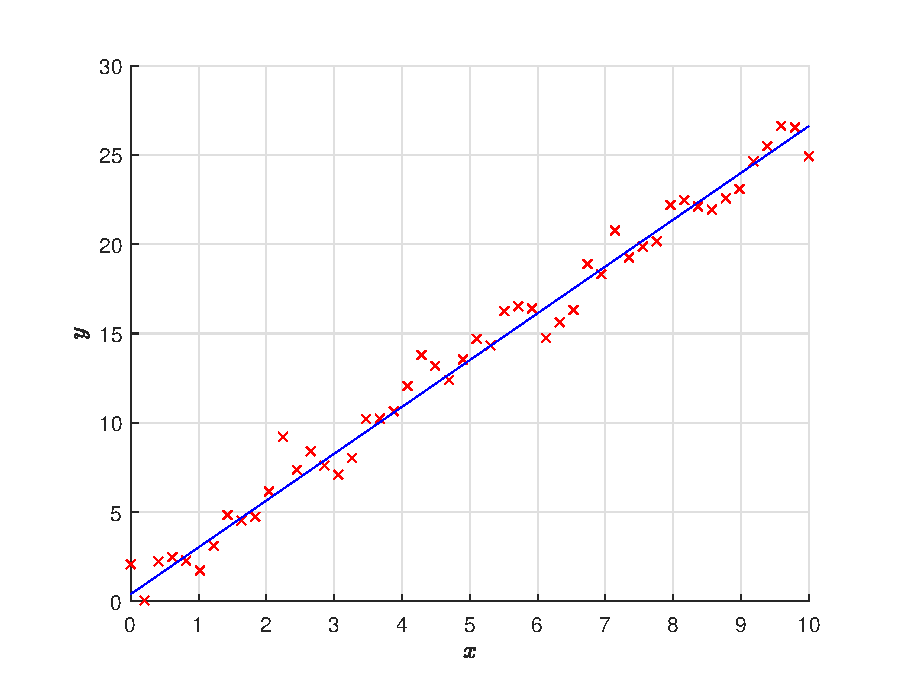
\includegraphics[width=0.6\textwidth]{chapters/part-1/figures/linear_regression_exp.eps}
	\caption{A demonstrative example for $1$-D linear regression, where a straight line is used to fit $50$ samples, with the results after $5$, $10$ and $20$ epochs of training are given by the blue dot line, dash dot line and solid lines respectively.} \label{fig:linear_regression_exp}
\end{figure}

During the training, the cost function \eqref{eq:linear_regression_solution_j} decreases as the line fits into the samples. This is reflected by Fig. \ref{fig:linear_regression_exp_j}. As a demonstration of how training improves the results, the intermediate result after $5$ epochs and $10$ epochs of training are given in Fig \ref{fig:linear_regression_exp} by the blue dot line and the blue dash dot line respectively.

\begin{figure}[!htb]
	\centering
	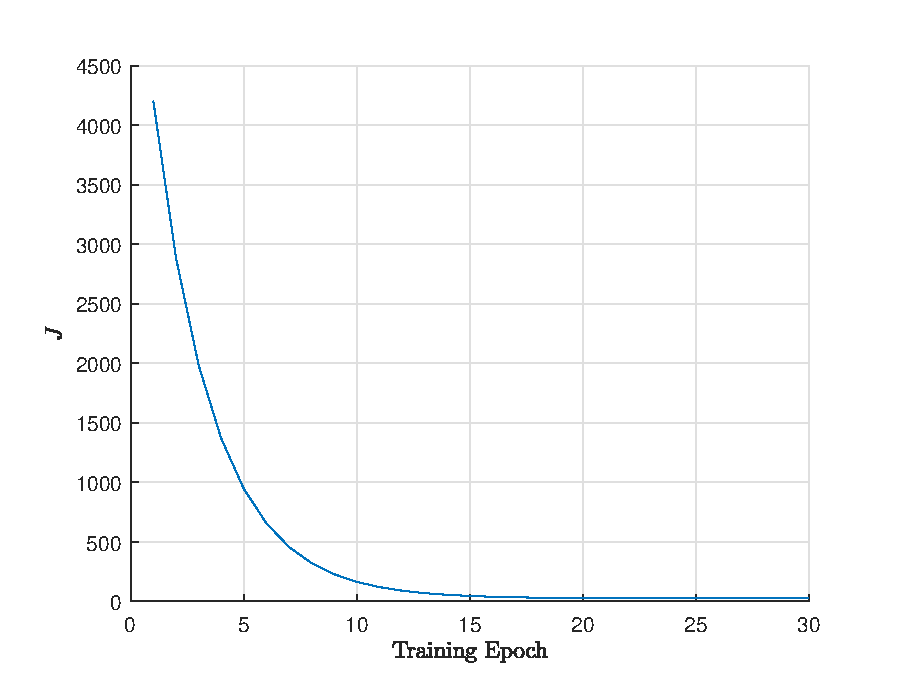
\includegraphics[width=0.6\textwidth]{chapters/part-1/figures/linear_regression_exp_j.eps}
	\caption{The decrement of the cost function during training.} \label{fig:linear_regression_exp_j}
\end{figure}

It is worth mentioning that the quadratic cost function $J$ given by \eqref{eq:linear_regression_solution_j} is a convex function of $\theta$ and $\theta_0$, and there is no local minimum. With a small learning rate $\alpha$, global minimum of $J$ can be achieved.

\subsection{Locally Weighted Regression}

Linear regression handles nonlinear samples by augmenting the feature vector. For example, assume that in \eqref{eq:linear_regression_problem} $f(x, \epsilon)$ is a nonlinear function of $x$, but a linear function of $x_i^2$ where $x_i$ is an element of $x$. In that case $x_i^2$ can be augmented into the features as follows.
\begin{eqnarray}
	\bar{x} &=& \left[x^T, x_i^2\right]^T \nonumber
\end{eqnarray}
and $f(\bar{x}, \epsilon)$ becomes linear to $\bar{x}$. In practice, it can be challenging sometimes to find the most appropriate set of features.

There are other methods to handle nonlinear samples mapping that are very close to linear regression. As an example, \mync{locally weighted regression} segments the samples into piece-wise neighborhoods, applies weighted linear regression for each neighborhood, and then aggregate the results. In each weighted regression corresponding with a neighborhood, each sample is assigned with a weight $0<w^i<1$ when performing weighted least squares in the linear regression. The closer a sample to the center of the neighborhood, the higher the weight. The weight is often calculated by
\begin{eqnarray}
	w_c^{(i)} &=& e^{-\frac{1}{2}(x^{(i)}-x_c)^T\Sigma_c^{-1}(x^{(i)}-x_c)} \nonumber
\end{eqnarray}
where $x_c$ is the center of a neighborhood, and $w_c^{(i)}$ the weight of a sample corresponding with that neighborhood. Scale parameter $\Sigma_c$ depends on the size of the neighborhood.

Locally weighted regression is effective when in the samples are piece-wise linear. Apparently, choosing the number of neighborhoods and their corresponding centers is critical to the algorithm.

Linear regression introduced in Section \ref{sec:linear_regression} is an example of \mync{parametric learning algorithm}, which has a fixed set of parameters $\theta$, $\theta_0$ in \eqref{eq:linear_regression} and the purpose of the machine learning is to fit them with most suitable values. In parametric learning algorithm, since the number of parameters is fixed regardless of the size of the training set, the memory consumption to trace and update the parameters is more or less limited.

Locally weighted regression, on the other hand, is a \mync{non-parametric learning algorithm}. The amount of parameters varies depending on the piece-wise segmentation which is decided by the number and position of the samples. The more and wider spread of sample, the more likely larger number of segments and parameters. 

\section{Logistic Regression}

Logistic regression, though has ``regression'' in its name, is genuinely considered as a binary classification method. 

\subsection{Problem Statement}

Let
\begin{eqnarray}
	y &=& f(x, \epsilon) \nonumber
\end{eqnarray}
where $y \in \{0,1\}$ is the label, $x\in\mathbb{R}^n$ the features, $n$ the number of features, $\epsilon$ the stochasticity of the model, and $f(\cdot)$ an unknown function of $x$. Notice that the label categories the samples into two categories, $0$ (negative) and $1$ (positive).

Linear regression \eqref{eq:linear_regression} cannot fit the labels efficiently. Consider using a non-linear mapping of the following format
\begin{eqnarray}
	h(x) &=& g\left(\theta^Tx\right) \label{eq:logistic_regression}\\
	&=& \dfrac{1}{1+e^{-\theta^Tx}} \nonumber
\end{eqnarray}
where
\begin{eqnarray}
	g(z) &=& \dfrac{1}{1+e^{-z}} \nonumber
\end{eqnarray}
is known as the \mync{sigmoid function} or \mync{logistic function} as shown in Fix \ref{fig:logistic_function}, and $\theta$ is the parameter vector to be fitted. 

\begin{figure}[!htb]
	\centering
	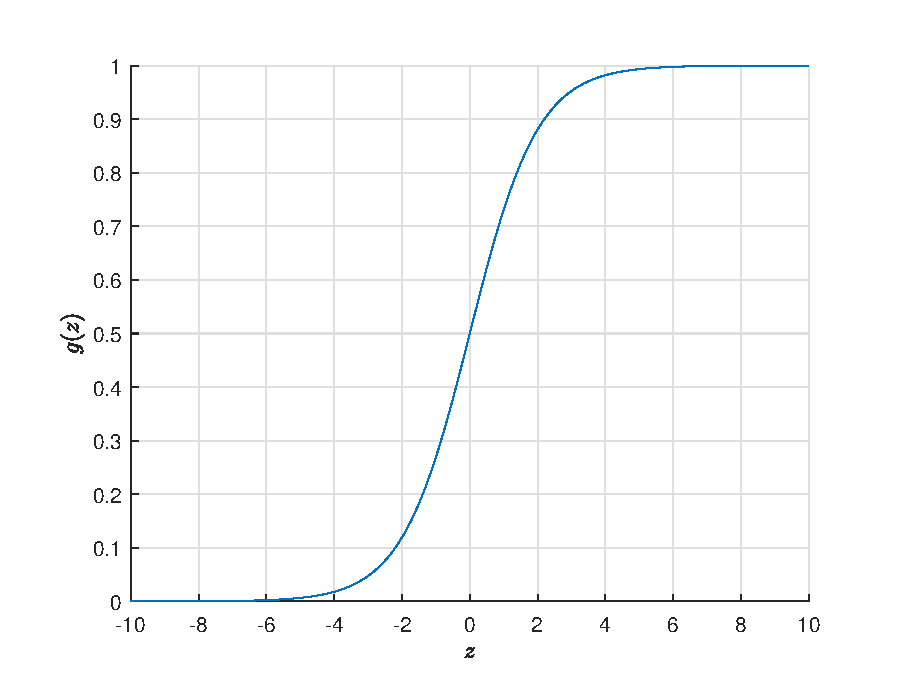
\includegraphics[width=0.6\textwidth]{chapters/part-1/figures/logistic_function.eps}
	\caption{Sigmoid function.} \label{fig:logistic_function}
\end{figure}

The hypothesis $0 < h(x) < 1$ due to the use of the sigmoid function, and it is used to map to the probability of $x$ being categorized with label $y=1$, i.e.,
\begin{eqnarray}
	P(y|x) &\approx& h(x)^y(1-h(x))^{1-y}, y\in\{0,1\} \label{eq:logistic_regression_probability}
\end{eqnarray}

If that can be done, the prediction of the category a new sample $x$ can then be determined by
\begin{eqnarray}
	\hat{y} &=& \left\{\begin{array}{cc}
		0 & h(x) \leq 0.5 \\
		1 & h(x) > 0.5
	\end{array}\right. \nonumber
\end{eqnarray}

\subsection{Solution with Gradient Descent}

As a first step, collect training samples. Let there be $m$ training samples denoted by $(x^{(i)}, y^{(i)})$, $i=1,\ldots,m$. Notice that $y^{(i)} \in \{0,1\}$, some of which taking positive values and others negative values.

Consider using maximum likelihood estimation to determine $\theta$. From \eqref{eq:logistic_regression} and \eqref{eq:logistic_regression_probability}, the likelihood of $\theta$ is given by
\begin{eqnarray}
	\mathcal{L}(\theta) &=& \prod_{i=1}^{m} \left[ h\left(x^{(i)}\right)^{y^{(i)}}\left(1-h\left(x^{(i)}\right)\right)^{1-y^{(i)}}\right] \label{eq:logistic_regression_mle1}
\end{eqnarray}
Maximizing \eqref{eq:logistic_regression_mle1} is equivalent with minimizing
\begin{eqnarray}
	J &=& - \mathrm{log}\left(\mathcal{L}(\theta)\right) \nonumber \\
	&=& - \sum_{i=1}^{m} \left[y^{(i)}h\left(x^{(i)}\right) + \left(1-y^{(i)}\right)\left(1-h\left(x^{(i)}\right)\right)\right] \label{eq:logistic_regression_mle2}
\end{eqnarray}

Consider using batch gradient descent to minimize \eqref{eq:logistic_regression_mle2} as follows
\begin{eqnarray}
	\theta &\leftarrow& \theta - \alpha \dfrac{\partial}{\partial \theta}J \nonumber
\end{eqnarray}
with $\alpha$ the learning rate and from \eqref{eq:logistic_regression_mle2}
\begin{eqnarray}
	\dfrac{\partial}{\partial \theta}L(\theta) &=& \sum_{i=1}^m \left[\left(h\left(x^{(i)}-y^{(i)}\right)\right)x^{(i)}\right] \label{eq:logistic_regression_gradient}
\end{eqnarray}

Notice that similar with the case of linear regression, \eqref{eq:logistic_regression_mle2} has no local maximum other than the global maximum.

One may notice that \eqref{eq:linear_regression_gradient} and \eqref{eq:logistic_regression_gradient} look similar regardless of how $h(x)$ is defined. This is not a coincidence. Though being two different algorithms, they both belong to a super-set algorithm. 



\include{chapters/part-2/ch_perceptron}

\include{chapters/part-2/ch_multilayer}

\part{Convolution and Recurrent Networks}

\include{chapters/part-3/ch_cnn}

\include{chapters/part-3/ch_rnn}

\part{Large Language Model}

\chapter{Transformer} \label{ch:transformer}

\myabb{Large language model}{LLM} is one of the many solutions to NLP, and NLP is a type of problem under sequential data processing. In the past few years we have seen revolutionary development in LLM, and hence it forms a dedicated part in the notebook. With the introduction of multimodal LLM, the capability of LLM expands beyond language processing towards image and even video processing. 

Modern LLM is built on top of Transformer, an AI framework proposed in the landmark paper ``Attention Is All You Need'' \cite{vaswani2017attention}. Transformer is introduced in this chapter. 

A brief review of RNN, the state-of-the-art framework prior to Transformer, is given, and its shortages are addressed. Transformer framework and its key components are introduced. Lastly, the development trend of Transformer is discussed.

\section{RNN and Its Limitations}

RNN has been introduced in earlier Chapter \ref{ch:rnn}. A brief review is given in this section, focusing on its shortages in NLP.

\subsection{A Brief Review of RNN}

Compared with a dense ANN, RNN is more efficient in building up correlation between consecutive inputs, and hence it becomes a powerful framework when it comes to sequential data processing. 

In a conventional dense ANN, the correlation cannot be captured efficiently. In contrast, a dense ANN would treat all the inputs ``equally'' in a symmetric manner. To enforce the ANN to ``address'' the correlation, it would require a lot more layers and nodes (which is often considered low-efficient), and requires more data points during the training. Other problems of conventional dense ANN include, for example, the lack of ability in handling data with arbitrary length.

CNN and RNN try to tackle the above problems by implementing a ``pre-processing'' stage, where the correlation of the spatial and sequential data is first abstracted using some mechanism, and the correlation information is sent as (additional) inputs to the following dense ANN.

\subsection{Limitations of RNN}

``Attention'' was not a new concept invented in \cite{vaswani2017attention}. It was proposed a few years earlier than the transformer, and had been integrated into several CNN and RNN models to boost their performances to capture long-range dependencies. In these researches, attention mechanism is more often a supporting role than the main character. It is quite surprising indeed that when getting rid of CNN and RNN and purely relying on attention mechanism, everything gets better: more efficient in training and better in performance.

Does this mean that the RNN, which we had been relying on so much, is in fact the drawback to NLP? The following is the answer of ChatGPT-4 of this question.

\begin{mdframed}
	\textbf{Q: By getting rid of RNN and using attention mechanism alone, natural language processing performance gets better. Is this correct? Does this mean that RNN is a drawback to natural language processing?}
	
	A: Yes, by getting rid of RNNs and using the attention mechanism alone, the Transformer model demonstrated improved performance in natural language processing tasks. However, it's important to note that RNNs are not inherently a drawback to NLP; they were successfully used for many tasks before the advent of Transformers.
	
	RNNs, particularly LSTM (Long Short-Term Memory) and GRU (Gated Recurrent Unit) variants, were designed to handle sequences and capture dependencies in the data. They have been effective in many NLP tasks, such as language modeling, machine translation, and sentiment analysis. However, RNNs do have certain limitations, such as difficulty in capturing long-range dependencies and sequential processing, which can lead to slower training and inference times.
	
	The attention mechanism, as employed in the Transformer model, addresses some of these limitations. It enables parallel processing of input sequences, leading to faster training and inference, and effectively captures long-range dependencies without the vanishing gradient problem that can affect RNNs.
	
	While Transformers have shown superior performance in many NLP tasks, RNNs still have their place in certain scenarios, especially when working with resource-constrained environments or smaller datasets. They can be more lightweight and computationally efficient compared to large-scale Transformer models.
	
	In summary, RNNs are not a drawback to NLP per se, but their limitations have been mitigated by the introduction of the attention mechanism in Transformer models, which has led to improved performance in a wide range of NLP tasks.
	
	(April 14, 2023, ChatGPT-4)
\end{mdframed}

\section{Transformer Framework}

A summary of the concepts, components and technologies in \cite{vaswani2017attention} is given in this section.

\subsection{Tokenizer}

In most NLP solutions, human language components need to be mapped to numbers before inputting into a model. The outputs of the model must then be mapped back to human-readable components so that a human can interpret them. This is no exception for LLMs. This mapping process is known as \mync{tokenization}.

There are multiple ways to perform tokenization. Different models, and models for different languages, may apply different tokenization schemes. In this section, English is used as an example. Commonly seen tokenization methods are discussed.

\vspace{0.1in}
\noindent \textbf{Character-Based Tokenization}
\vspace{0.1in}

The most intuitive approach is character-based tokenization. For example, we can use the ASCII standard as the mapping table, where each English character, including spaces and most commonly used special characters, is mapped to an integer.

The benefits of using character-based mapping include:
\begin{itemize}
	\item Flexibility. Everything can be mapped without exception, including typos or invented words.
	\item Compact vocabulary. To cover all characters, we need only a few dozen entries in the mapping table.
\end{itemize}

The main drawback of character-based mapping is inefficiency. For instance, consider the character sequence ``t'', ``h'', and ``e''. When they appear together, they form the word ``the'' which carries a specific and frequent meaning. Ideally, such frequent patterns should be recognized as a whole. By storing this combination in the token mapping (rather than learning it from model parameters), we can improve modeling efficiency and reduce sequence length.

\vspace{0.1in}
\noindent \textbf{Word-Based Tokenization}
\vspace{0.1in}

To improve efficiency and reduce the number of input tokens, word-based tokenization was proposed. A dictionary containing around $30{,}000$ to $50{,}000$ words is often used in common applications. Any unrecognized word such as typo or extremely rare word is mapped to a special token that represents an ``unknown'' word.

The advantages of word-based mapping include:
\begin{itemize}
	\item Efficiency. Fewer tokens are needed to represent a sentence compared to character-level mapping.
	\item Better contextual grounding. Each token usually corresponds to a semantically meaningful unit.
\end{itemize}

However, word-based tokenization sacrifices flexibility. Unseen or misspelled words provide no meaningful signal other than ``unknown''. 

Additionally, word-based schemes often ignore the semantic structure within a word. For example, consider the word ``handcraft''. It is clearly composed of two recognizable words ``hand'' and ``craft''. Semantically, ``handcraft'' relates to both. Yet, in the word-based mapping, ``hand'', ``craft'' and ``handcraft'' are treated as entirely unrelated tokens. In such cases, it would be more effective to break the word into meaningful segments and tokenize those instead.

\vspace{0.1in}
\noindent \textbf{Subword-Based Tokenization}
\vspace{0.1in}

Modern LLMs typically use subword-based tokenization. This approach lies between character-based and word-based methods. It tries to achieve optimum flexibility and efficiency by smartly breaking a word into semantically meaningful chunks known as ``subwords''.

An example is given in Fig. \ref{fig:tokenizer}, where a small piece of text is tokenized using a tokenizer. From the example, we can see that while basic and commonly used words such as ``I'', ``am'', ``demonstrating'', ``sentence'' remain in one token, the sophisticated words such as ``OpenAI'', ``tokenization'', ``semantically'' are broken into subwords. Notice that spaces and special characters such as period ``.'' are also considered as part of tokens, as they carry meanings.

\begin{figure}[!htb]
	\centering
	\includegraphics[width=0.75\textwidth]{./chapters/part-4/figures/tokenizer.png}
	\caption{A demonstrative example where a piece of text is tokenized using GPT-4o's tokenizer.}
	\label{fig:tokenizer}
\end{figure}

Each token is then assigned with a token ID. In the example in Fig. \ref{fig:tokenizer}, they are
\begin{lstlisting}
[40, 939, 73405, 6602, 2860, 328, 40536, 2360, 7788, 17527, 885, 6361, 13, 730, 290, 6602, 2860, 11, 261, 21872, 382, 17162, 1511, 2743, 175665, 33329, 1543, 10020, 13, 256]
\end{lstlisting}

Subword tokenization allows the model to:
\begin{itemize}
	\item Represent rare or unknown words by combining familiar parts (e.g., prefixes, stems, suffixes).
	\item Reduce the number of out-of-vocabulary tokens. Even if a new word or typo is detected in the text, it is possible that it still contains meaningful subwords.
	\item Maintain a compact vocabulary while preserving semantic structure.
\end{itemize}

Just to put things into perspective, for a typical tokenizer on English writing, $1$ token is roughly $4$ characters, or $0.75$ word, and $1000$ tokens are roughly $750$ words. Nowadays, math equations, scientific terms and codes are also used as inputs and outputs to LLMs for domain knowledge related tasks. They usually consumes more tokens than English writings.

Different LLMs may use different tokenizers. Popular subword techniques include Byte Pair Encoding, WordPiece, and Unigram tokenization. The example in Fig. \ref{fig:tokenizer} demonstrates the tokenizer of OpenAI's GPT-4o. There are many other tokenizers used by variety of models. At this point, there is not a universally best tokenizer.

The maximum number of tokens an LLM can process, both as input and output, is limited by its \mync{context window}. For example, consider a continuous dialogue with an LLM-based chatbot. Each time the user provides a new input, the entire chat history (including all of the user's previous inputs and the LLM's previous responses) is bundled together and sent as a new stateless input to the model. Based on this complete input sequence, the LLM then generates its latest response. This stateless nature means that the LLM does not ``remember'' anything beyond what is explicitly included in the current input. 

As the conversation grows longer, more and more tokens are needed to represent the chat history. For example, GPT-4o model has a context window of $128K$ tokens, roughly one-tenth the length of the complete works of Shakespeare. Once this limit is reached, older parts of the conversation must be truncated or summarized.

In some scenarios, the input cannot be easily compressed or truncated and must be passed to the LLM as a whole. For example, when an LLM is used to troubleshoot a piece of code, the entire code block, possibly including multiple files, configurations, and logs, needs to be input at once to maintain context and correctness. In such cases, the size of the context window becomes a critical constraint. If the total input exceeds the model's maximum token limit, the model will either fail to process it entirely or may be forced to omit important parts of the input, potentially leading to incorrect or incomplete responses.



\subsection{Encoder and Decoder}

TBA

\subsection{Attention Mechanism}

TBA

\subsection{Transformer-Based NLP}

\section{Transformer Development Trend}

\subsection{Transformer Variants}

\subsection{Trend}

With the sizes and capabilities of the frontier models scaling up over the past years, the models are more and more appear to be intelligent and human-like. 

A new job opportunity, ``prompt engineer'', has emerged. The workscope of a prompt engineer is to design the appropriate prompt that instructs an LLM to complete certain tasks accurately and efficiently. People starts to take advantage of LLMs in their production. 

Today, some most popular LLM applications include at least the following.
\begin{itemize}
  \item Chatbot and customer service.
  \item Copilot
  \item Agentization
\end{itemize} 

\chapter{Large Language Model: Theory} \label{ch:llmtheory}

This chapter serves as an overview of the large language model from the theory and technical perspective. LLM is a successful practice of NLP and beyond. It can not only process human languages but also generate new contents based on human language written requirements. The introduction of multimodal LLM further allows LLM to understand and generate not just writings but also pictures and videos.

Nowadays, it is possible for a regular user to leverage on commercialized models to develop his own applications. Given a powerful machine, a user can even deploy LLMs locally in a few steps. Open-source LLMs are available so that the user does not need to train a model from scratch. The deployment of LLMs and the interaction with them are introduced in the next Chapter \ref{ch:llmpractice}.

Modern LLMs are built on top of Transformer framework which has been introduced in earlier Chapter \ref{ch:transformer}. It is worth emphasizing the relationship between the Transformer and LLM. Transformer is an ANN framework designed for processing any sequential data so long as it can be encoded, and apparently NLP is an important use case of it. LLM is a practice of Transformer on NLP.

\section{Introduction to LLM}

This section reviews existing NLP methods and their limitations, and discusses the gaps that LLM bridges.

\subsection{Existing NLP Models and Gaps}

There have been variety of ways to model natural languages. For example, consider the following sentence:
\begin{center}
	\textit{``I am thirsty. Please give me a bottle of \rule{1cm}{0.15mm}.''}
\end{center}
It is quite natural that a human would likely to put ``water'' or ``tea'' in the blank. This is obvious because human has a dictionary of words that he can choose in his mind, and he has been reinforced of learning ``a bottle of water'' expression in many occasions. In addition, it makes sense to a human that when someone is thirsty, he would look for water.

The challenge using AI on the above task is to build the ``dictionary'' in the machine and quantitatively analyze what word or phrase would make the most sense to be filled into the blank. Many models have been proposed to solve this problem, some of which have been evolving over time in the past decades since $1990$th.

\vspace{0.1in}
\noindent \textbf{Statistical Language Models}
\vspace{0.1in}

In the early days when AI and ANN were not popular, \mync{statistical language models}[SLM] have been the most popular tool to model natural languages. SLM assumes that a sentence is a Markov process, and the last word depends on the context created by the most recent $n$ words. SLM with a fixed context length of $n$ is also called an $n$-gram language model.

Conventionally, the paring information from $n$ words to the next word is obtained from data corpus and stored in a table-like structure. When running the model, it looks up the table for the most probable next word based on the earlier $n$ words. Smoothing technologies are used to handle zeros, i.e., when the record is not found in the table.

An obvious issue of SLM is that the computation and storage of the model increase exponentially with the size of $n$. This limits the context information that the model can use for prediction, hence setting a low performance ceiling. Not to mention that even with a large data corpus, zeros can still happen and the model performance is always an issue in such occasions.

\vspace{0.1in}
\noindent \textbf{Neural Language Models}
\vspace{0.1in}

With the introduction of ANN, in particular RNN, \mync{Neural Language Models}[NLM] became popular. RNN-based NLM builds the word prediction function conditioned on the aggregated context features abstracted and passed recurrently from current and previous input sequence. More about RNN has been introduced in Chapter \ref{ch:rnn}.

RNN is not a perfect one-stop solution either. The training of RNN can be difficult due to vanishing and exploding gradient problems. This limits the depth that RNN can go. When handling long sequence of words, the performance of RNN drops significantly because it is weak at building long-term dependencies.

\vspace{0.1in}
\noindent \textbf{Pre-trained Language Models and Large Language Models}
\vspace{0.1in}

As introduced in details in earlier chapters, attention mechanism has been proposed to tackle the long-term dependency problem of RNN. Transformer architecture, which relies purely on encoder, decoder and attention mechanism without using RNN is then proposed. It has been verified that transformer architecture is good at abstracting information from sequential data, in particular, natural languages. With a transformer, it becomes possible to build very deep neural networks and have it trained efficiently with big-size data corpus. The outcome is known as the \mync{large language model}[LLM].

Language models based on different transformer-based architectures are often called \mync{Pre-trained Language Models}[PLM]. LLM can be taken as a subset of PLM. The main difference between an LLM and a regular PLM is the size of the model. The scaling of the model from hundreds of millions of parameters for PLMs to tens or hundreds of billions of parameters for LLMs introduces emergent abilities such as in-context learning to the model, significantly enhancing its capability and intelligence. As of this writing, it is not very clear how the these abilities suddenly emerge with the size of the model.

\subsection{LLM Features and Capabilities}

When the size of the model becomes large, usually to the order of at least a few billions parameters, they suddenly gain emergent abilities. Details are discussed as follows.

\vspace{0.1in}
\noindent \textbf{In-context Learning}
\vspace{0.1in}

\mync{In-Context Learning}[ICL] allows the behavior of the model to be manipulated via not training or fine-tuning of the parameters, but via instructions and demonstrations given as part of the input.

ICL plays an important part in LLM implementation, as it is the basis of prompt engineering. When the LLM is large, it is possible to use prompt engineering instead of fine-tuning to complete a task following user defined instructions. This reduces the training cost and makes the implementation more flexible.

\vspace{0.1in}
\noindent \textbf{Instruction Following}
\vspace{0.1in}

Supervised learning is commonly used in training and fine-tuning a model. In the training set, we need to provide the model ``examples''. An example includes the input, some good responses, and some bad responses. 

When comes to LLM, it is possible to fine-tune a model for a specific task without using the aforementioned examples. Instead, just give it step-by-step instructions. LLM is able to perform well with these tasks described only by instructions. This is known as instruction tuning.

It is worth mentioning that instruction following is also possible in ICL. Give the LLM instructions in prompt engineering without examples, and the LLM is likely to be able to finish the tasks.

\vspace{0.1in}
\noindent \textbf{Step-By-Step Reasoning}
\vspace{0.1in}

When a model is asked to complete a complicated task that involves multiple steps, it may fail to accomplish the task. With a well fine-tuned LLM, the model might be able to break the task into multiple sub-tasks via \myabb{chain-of-thought}{CoT} prompting strategy, and solve them step-by-step till the final result is obtained.

It has been observed that an LLM with at least $100B$ parameters is likely to have good step-by-step reasoning abilities.

The performance of an LLM, usually referring to its capability in accurately and correctly complete a task, is affect by many factors such as the model architecture, model size, training data set size and quality, etc. Though it is clear that with the scaling up of the system the performance is usually improved, there is no analytical expression that gives full insights about how these factors affect the performance quantitatively.

A \mync{scaling law} tries to quantitatively describe the performance of an LLM as a function of model size and other factors. Many scaling laws have been proposed, many of which obtained from empirical experiments and they may work only within a given range of model size.

Just as an example, OpenAI proposed KM scaling law in 2020 that describes LLM cross entropy loss as a function of model size, training data set size and training computation as follows.
\begin{eqnarray}
	L(N) &=& \left(\dfrac{N_c}{N}\right)^{\alpha_N} \nonumber \\
	L(D) &=& \left(\dfrac{D_c}{D}\right)^{\alpha_D} \nonumber \\
	L(C) &=& \left(\dfrac{C_c}{C}\right)^{\alpha_C} \nonumber
\end{eqnarray}
where $N$, $D$ and $C$ denote the model size, dataset size and training computation, respectively. The rests are constants whose value can be obtained via calibration.

This scaling law works for models with $22M$ to $23B$ parameters. It is assumed that the analysis of a factor can be done independently without other parameters being a bottleneck.

\subsection{LLM Performing Benchmarks}

\subsection{LLM Development Timeline}

A brief timeline of the development of LLMs since the publication of \cite{vaswani2017attention} is given below.

\vspace{0.1in}
\noindent \textbf{2017}
\vspace{0.1in}

``Attention Is All You Need'' \cite{vaswani2017attention} introduced a new type of NLP model called the ``Transformer''. Unlike traditional RNN-based models, the Transformer removes all recurrent components and adopts an encoder-decoder architecture that relies entirely on self-attention mechanisms to model dependencies within and across sequences.

\vspace{0.1in}
\noindent \textbf{2018-2020}
\vspace{0.1in}

OpenAI released the GPT-1, GPT-2, and GPT-3 models in consecutive years from 2018 to 2020, showcasing the scalability of Transformer-based architectures for autoregressive language modeling.

\vspace{0.1in}
\noindent \textbf{2022}
\vspace{0.1in}

\myabb{Reinforcement Learning from Human Feedback}{RLHF} became a widely adopted training strategy. OpenAI released ChatGPT, a chatbot fine-tuned from the GPT-3.5 model using RLHF. Its human-like conversational abilities captured public attention and spurred a surge of interest and development in LLM-based applications.

\vspace{0.1in}
\noindent \textbf{2023-2024}
\vspace{0.1in}

GPT-4, GPT-4o are published in 2023 and 2024 respectively, along with many other frontier models are published.

\subsection{LLM-Relevant Milestone Technologies}

This section looks back into the progression tree of LLM, and lists down milestone techniques that make LLM what it is today. It is the breakthrough in these areas that revolutionizes LLM development.

\vspace{0.1in}
\noindent \textbf{Big Data}
\vspace{0.1in}

The performance of LLM relies on both the modal size and the training data size. It is the advent in internet, Web 3.0, Industry 4.0, IoT and cloud computing/storage that makes collection and aggregation of big data possible.

Almost every large-size enterprise, both IT companies and conventional industrial companies, have their internal databases. The database can be used to train domain-knowledge LLM. Nowadays, there are many open data sources of community LLMs. Such examples include BookCorpus, CommonCrawl, Reddit posts (with high upvotes), Wikipedia, and many more. These open-source datasets make training LLM for community projects possible.

\vspace{0.1in}
\noindent \textbf{Large Model and Efficient Training}
\vspace{0.1in}

The invention of CPU-based neural networks and transformer architecture making creating and training large scale LLM possible. Both closed and open-source LLMs have been proposed, including GPT series by OpenAI and LLaMA family by Meta AI and the community.

Manly libraries have been released to the public to help building, training and fine-tuning LLMs, such as \verb|transformers|, a Python library for building transformer models. Many such libraries are tying up with PyTorch and TensorFlow to provide LLM related functions.

More about these models and libraries are introduced in later sections.

\vspace{0.1in}
\noindent \textbf{Fine-Tuning}
\vspace{0.1in}

Technologies such as LoRA has made fine-tuning easier than before.

\vspace{0.1in}
\noindent \textbf{Prompt Engineering}
\vspace{0.1in}

There have been a lot of practices on how to make LLM flexible and more efficient in solving particular tasks via prompt engineering.

\vspace{0.1in}
\noindent \textbf{LLM on Edge Devices}
\vspace{0.1in}

Many efforts have been put into edge-device based LLMs. The target is to develop LLM that consumes less memory, storage and computation while not sacrificing a lot of performance.

\vspace{0.1in}
\noindent \textbf{API and Interface}
\vspace{0.1in}

Multi-modal LLM has enabled different types of inputs to the LLM, not limited to natural language but also sequential signals and even pictures.

Many tools and software have developed APIs for LLM. These tools enhance computation and online information retrieval capabilities of LLM.

\section{Existing LLMs Features}

As of this writing, there are countless LLMs available on the market or within the open-source community, and the list continues to evolve rapidly. 

This section introduces the shared properties and general characteristics of existing LLMs, without delving into detailed performance metrics or task-specific comparisons. The goal here is not to promote one model over another, but rather to provide a broad overview of what defines an LLM in practice.

A more detailed performance review of selected models is provided in Section~\ref{sec:frontierllmmodels}.


Many LLMs are capable of engaging in human-like conversations and answering questions in depth. Some can even search the internet for the up-to-date relevant information to support their responses. Most well-known LLMs can also follow user instructions to perform specific tasks, such as completing a piece of code, provided the prompts are sufficiently clear and aligned with the model's training data.

That said, many LLMs (unless specifically trained on domain-specific corpora) do not perform as well as experienced professionals in specialized fields. It is often claimed that top-performing LLMs can achieve a level of performance comparable to fresh PhD graduates in certain tasks, although a noticeable gap remains when compared to experienced researchers.

LLMs may generate inaccurate or misleading information while expressing it in a fluent and confident manner. This behavior stems from the their lack of self-awareness and inability to judge the factual correctness of its outputs.

LLMs can also struggle with detailed quantitative tasks. This limitation arises from how they process and generate language: input is tokenized into subword or word-like units, and outputs are generated based on statistical patterns rather than precise symbolic reasoning. For example, an LLM might fail to correctly answer a seemingly simple question like ``How many letters `a' are there in this sentence?'', because its training does not emphasize accurate character-level counting.

Multimodal LLMs can generate images or videos based on textual descriptions. However, they often struggle to accurately render fine-grained visual details. For example, if prompted to generate an image of a car with a license plate that reads ``3.14159265358979'', the resulting image may omit or distort some of the digits. This limitation stems from the fact that image generation is driven by probabilistic pattern synthesis, not precise symbolic encoding or controlled rendering of visual elements. An example is given in Fig. \ref{fig:gpt_carplate}.

\begin{figure}[!htb]
	\centering
	\includegraphics[width=0.5\textwidth]{./chapters/part-7/figures/gpt_carplate.png}
	\caption{A figure from a GPT when it is asked to generate a car with a license plate that reads ``3.14159265358979''.}
	\label{fig:gpt_carplate}
\end{figure}

It is true that each LLM is trained and fine-tuned with different data corpus and may behave differently on different types of tasks. Consider LLMs with the same model structure and training strategy. In such case, models with larger training data sets and more parameters often outperform those with smaller training data sets and less parameters. From application perspective, the trend is that the frontier models' performances are converging for regular tasks, and the costs are going to be the main differentiator. 

OpenAI's GPT models and Meta's LLaMA models are the first models that gain popularity. A brief review is given in the remaining of the section.

\subsection{OpenAI Family}

OpenAI started investigating language models before the proposition of transformer. In its early days, RNN was explored as the most promising model for natural language. In 2017 when the transformer model was proposed, OpenAI quickly adapted their language model to this new architecture, and as a result generative pre-training (GPT) series has been proposed.

\vspace{0.1in}
\noindent \textbf{GPT-1}
\vspace{0.1in}

GPT-1, OpenAI's first transformer based PLM was proposed in 2018. GPT-1 has $117M$ parameters in the model and it adopts a decoder-only architecture, which is different from the original transformer proposal which has a encoder-decoder architecture. GPT-1 was trained via a two-stage procedure, the first stage unsupervised pre-training and the second stage supervised fine-tuning. This two-stage training pipeline, or something of the similar kind, has been adopted by many LLMs coming after.

\vspace{0.1in}
\noindent \textbf{GPT-2}
\vspace{0.1in}

GPT-2 is an improvement of GPT-1. It uses much larger number of parameters of $1.5B$ in the model, and it was trained on a much larger dataset WebText. With larger model and training data size, GPT-2 is targeted to be a multi-task solver. The model can be formulated by the following probabilistic form
\begin{eqnarray}
  \textup{Pre-trained LLM} &\equiv& P\left(\textup{output}\middle|\textup{input}, \textup{task}\right) \nonumber
\end{eqnarray}
In the above formulation, each NLP task can be considered as the word prediction problem based on a subset of the word next, and can be trained during the unsupervised learning stage. Unsupervised pre-training has since then become the most important stage for the LLM to gain knowledge for general tasks.

\vspace{0.1in}
\noindent \textbf{GPT-3, GPT-3.5 and Chat-GPT}
\vspace{0.1in}

It is clear now that GPT-2 has $1.5B$ parameters which is too few for an LLM to gain emergent abilities. It is GPT-3 with $175B$ parameters trained on $300B$ tokens that made a capability leap and bring LLM to everyone's attention.

It is GPT-3 that for the first time introduces emergent abilities such as ICL. GPT-3 not only accomplishes commonly seen tasks to test LLM capabilities with flying color, but also demonstrates features not shown by other models before, such as reasoning and domain adaption.

OpenAI has developed many task-oriented models that use GPT-3 as the base model. For example, for coding, Codex was introduced. Codex is basically GPT-3 fine-tuned using code database such as GitHub. Comparing with GPT-3, Codex is able to reason and solve complex mathematical problems, and realize them in codes. RL had already been used to fine-tune and improve performance for GPT-2. The same has been applied on GPT-3. Furthermore, reinforcement learning with human feedback (RLHF) is introduced for GPT-3 that allows the model to continue learning from human demonstrations.

With the above enhancements, i.e. code-based fine-tuning, RL and RLHF, GPT-3.5 has been developed. GPT-3.5 is an enhanced version of GPT-3 and it is obtained from GPT-3 via transfer learning. GPT-3.5 is also scaled up in size, with a parameter number of $335B$.

Chat-GPT was developed on top of GPT-3.5 (and later another version was released developed on top of with GPT-4). It is GPT-3.5 fine-tuned specially optimized for dialogue. It demonstrates how LLM can be used in everyone's daily life as an assistant, consultant and a copilot. Chat-GPT demonstrated good performance in communicating of humans than other GPT models. This is because Chat-GPT is trained on human-generated conversations of both human and AI roles. Later on, plug-ins and APIs are enabled on Chat-GPT, to allow it to communicate with other software.

\vspace{0.1in}
\noindent \textbf{GPT-4}
\vspace{0.1in}

GPT-4 is a multimodal LLM, meaning that it can not only take in natural languages, but also other signals such as images. Comparing with GPT-3.5, GPT-4 demonstrates further enhanced capabilities. It is claimed that GPT-4 is safer to use and is less likely to generate toxic and misleading information.

Just as a quick demonstration of its multimodal feature, pass the following Fig. \ref{fig:superpower_cat} (notice that this figure itself is generated by an AI model) to GPT-4 with instruction ``What is in this picture?''. GPT-4 is able to response the following:

\vspace{0.1in}
\noindent \textit{``The image showcases a majestic cat standing in a fantastical landscape. The cat emits a luminous, ethereal glow, and its fur and tail appear to be infused with swirling, fiery or cosmic energies in brilliant hues of red and gold. These radiant swirls surround the cat, adding to its supernatural aura. Behind the cat, there's a dramatic night sky with clouds illuminated by a hidden light source, possibly lightning or a celestial event. In the foreground, the terrain appears to be a combination of grassy knolls and fiery, ember-lit ground, further emphasizing the magical and otherworldly nature of the scene. The entire setting evokes a sense of wonder and fantasy.''}
\vspace{0.1in}

\begin{figure}[!htb]
	\centering
	\includegraphics[width=0.6\textwidth]{./chapters/part-7/figures/superpower_cat.png}
	\caption{A cat with superpower. This picture is generated by DALL$\cdot$E 3.}
	\label{fig:superpower_cat}
\end{figure}

\vspace{0.1in}
\noindent \textbf{Other OpenAI Models}
\vspace{0.1in}

DALL$\cdot$E is the model OpenAI uses to generate images. As of this writing, its latest version, DALL$\cdot$E 3, has been integrated with the latest ChatGPT. Figure \ref{fig:superpower_cat} gives an example where DALL$\cdot$E 3 is used to generate a image of a superpower cat.

OpenAI Codex, as introduced earlier, is the GPT model optimized for code generation. As of this writing, Codex has been deprecated because its capability has been integrated into ChatGPT. It is possible to ask ChatGPT to generate a piece of code following user's instruction and description.

OpenAI Codex is the engine that powers GitHub copilot. In this sense, OpenAI Codex remains a live in a different format: not as a standalone software or model, but more as an API.

\subsection{LLaMA Family}

Large Language Model Meta AI (LLaMA) is the LLM model developed by Meta AI. Different from most of the AI models (GPT-3 and onward) developed by OpenAI, LLaMA is open-source hence has a wide availability. Many efforts in the community have made modifications and improvements to LLaMA, making a big family of models with different characteristics.

As of this writing, a family tree of LLaMA is shown in Figure \ref{fig:llama_family_tree}. The picture is from \cite{zhao2023survey}. The source of the picture is given in the GitHub repository of the paper.
\begin{figure}[!htb]
	\centering
	\includegraphics[width=\textwidth]{./chapters/part-7/figures/lamma_family_tree.png}
	\caption{LLaMA family tree.}
	\label{fig:llama_family_tree}
\end{figure}
Only a small portion of models in the family tree is briefly introduced here.

\vspace{0.1in}
\noindent \textbf{LLaMA}
\vspace{0.1in}

LLaMA, comparing with GPT-3 which was used as a benchmark, is smaller in model size (maximum $65B$ parameters VS $175B$ parameters in GPT-3) but larger and better in training data size and quality (maximum $1.4T$ tokens VS $300B$ tokens in GPT-3). As a result, LLaMA is able to achieve generally better performance than GPT-3 with less implementation cost due to the small size. LLaMA demonstrates that training data is equality important as model size. It is possible to reach the same level of performance with a small ($<100B$ parameters) but well-trained model.

LLaMA's first release includes 4 models of different model and training sizes. Details are summarized in Table \ref{ch:llm:tab:llamamodels}.
\begin{table}[!htb]
	\centering \caption{LLaMA models.}\label{ch:llm:tab:llamamodels}
	\begin{tabular}{ccc}
		\hline
		Name & Model Size & Training Dataset Size \\ \hline
		LLaMA 7B & $6.7B$ & $1T$ \\
		LLaMA 13B & $13.0B$ & $1T$ \\
		LLaMA 33B & $32.5B$ & $1.4T$ \\
		LLaMA 65B & $65.2B$ & $1.4T$ \\
		\hline
	\end{tabular}
	\begin{flushleft}
		\footnotesize
		Model size is given in number of parameters in billion. Training data size is given in number of tokens.
	\end{flushleft}
\end{table}
The training dataset is purely open-source, including Common Crawl, C4 Dataset, GitHub, Wikipedia, public domain books, arXiv and Stack Exchange.

Technical wise, LLaMA has some innovations on top of the original transformer proposition \cite{vaswani2017attention} n the normalization method, activation function, and embedding methods. More details will be introduced in later sections.

Many open-source tools and packages have been developed to fine-tune LLaMA and its variations. More about fine-tuning, such as LoRA\cite{hu2021lora} and QLoRA\cite{dettmers2023qlora}, are introduced in more details in later sections. Notice that fine-tuning or re-training of a model often cost a lot of computational power and vector memory.

\vspace{0.1in}
\noindent \textbf{Stanford Alpaca}
\vspace{0.1in}

Stanford Alpaca 7B is Standford's practice in fine-tuning LLaMA 7B. The running cost of this fine-tuning is impressively small (hundreds of USD), and the resulted model has a performance comparable with GPT-3.5 which has $335B$ parameters. It is impressive to see that a small $7B$ model can compete with a large $335B$ model by careful training and fine-tuning. This might be partially because Alpaca 7B is fine-tuned from LLaMA 7B using knowledge distillation from GPT-3.5 (also known as text-davinci-003).

The details of training Stanford Alpaca can be found in \cite{alpaca}. A brief highlight is given below. The fine-tuning pipeline of Alpaca is shown in Fig. \ref{fig:alpaca_pipeline}. It is a 2-stage process as follows.
\begin{enumerate}
	\item Generating instruction-following examples using GPT-3.5 (text-davinci-003).
	\item Fine-tune LLaMA 7B using the examples.
\end{enumerate}
\begin{figure}[!htb]
	\centering
	\includegraphics[width=\textwidth]{./chapters/part-7/figures/alpaca_pipeline.jpg}
	\caption{Alpaca fine-tuning pipeline.}
	\label{fig:alpaca_pipeline}
\end{figure}

Examples of the generated instruction and response pairs are given below. The full list is available from the GitHub repository.
\begin{lstlisting}
{
	"instruction": "What are the three primary colors?",
	"input": "",
	"output": "The three primary colors are red, blue, and yellow."
},
{
	"instruction": "Give three tips for staying healthy.",
	"input": "",
	"output": "1.Eat a balanced diet and make sure to include plenty of fruits and vegetables. \n2. Exercise regularly to keep your body active and strong. \n3. Get enough sleep and maintain a consistent sleep schedule."
},
{
	"instruction": "Extract the facts from the paragraph.",
	"input": "Online education continues to become more popular for schools and students alike. Its advantages are generally lower costs, less commitment and the ability to study at a time, place and pace that suits the student.",
	"output": "- Online education is becoming increasingly popular.\n- It has several advantages such as lower costs, less commitment and the ability to study at one\u2019s own time and pace."
},
{
	"instruction": "Arrange the given numbers in ascending order.",
	"input": "2, 4, 0, 8, 3",
	"output": "0, 2, 3, 4, 8"
}
\end{lstlisting}

The fine-tuning code of Alpaca is from Hugging Face. Python packages such as \verb|numpy|, \verb|torch|, \verb|transformers|, etc., are required. Check \verb|requirements.txt| and \verb|train.py| in the repository for more details. Call \verb|train.py| using something like the following
\begin{lstlisting}
torchrun --nproc_per_node=4 --master_port=<your_random_port> train.py \
	--model_name_or_path <your_path_to_hf_converted_llama_ckpt_and_tokenizer> \
	--data_path ./alpaca_data.json \
	--bf16 True \
	--output_dir <your_output_dir> \
	--num_train_epochs 3 \
	--per_device_train_batch_size 4 \
	--per_device_eval_batch_size 4 \
	--gradient_accumulation_steps 8 \
	--evaluation_strategy "no" \
	--save_strategy "steps" \
	--save_steps 2000 \
	--save_total_limit 1 \
	--learning_rate 2e-5 \
	--weight_decay 0. \
	--warmup_ratio 0.03 \
	--lr_scheduler_type "cosine" \
	--logging_steps 1 \
	--fsdp "full_shard auto_wrap" \
	--fsdp_transformer_layer_cls_to_wrap 'LlamaDecoderLayer' \
	--tf32 True
\end{lstlisting}
where \verb|./alpaca_data.json| is the JSON file that contains all the instruction and response pairs.

Notice that later on, Stanford Alpaca 13B is also developed based on LLaMA 13B.

\vspace{0.1in}
\noindent \textbf{Vicuna}
\vspace{0.1in}

Vicuna 13B is an open-source chatbot fine-tuned on top of LLaMA using $70K$ user-shared conversations collected from ShareGPT (a platform where users share their ChatGPT conversation histories). Its performance is comparable with GPT-3.5 and Bard, and it is slightly better than LLaMA 13B and Alpaca 13B in general.

See \cite{vicuna2023} for more details.

\vspace{0.1in}
\noindent \textbf{LLaVA and MiniGPT-4}
\vspace{0.1in}

Large Language and Vision Assistant (LLaVA) is a multimodal LLM that combines a vision encoder and Vicuna for general purpose visual and language understanding. More details are given in \cite{liu2023llava} and \cite{liu2023improvedllava}. Similar with GPT-4, its multimodal encoders allows it take both natural language and image as inputs. An example is given below.

Pass the same Fig. \ref{fig:superpower_cat} to LLaVA with the same instruction ``What is in this picture?''. LLaVA is able to give the following response:

\vspace{0.1in}
\noindent \textit{``The image features a cat standing on a hill, with a fiery background and a cloudy sky. The cat appears to be looking at the viewer, and there is a sense of motion in the scene.''}
\vspace{0.1in}

Similar with LLaVA, MiniGPT-4 is a also multimodal LLM that enhances vision interpretation. More details are given in \cite{zhu2023minigpt}. It uses different techniques and realizations from LLaVA. Pass the same Fig. \ref{fig:superpower_cat} to MiniGPT-4 with the same instruction ``What is in this picture?''. MiniGPT-4 is able to give the following response:

\vspace{0.1in}
\noindent \textit{``The image shows a white cat with flames coming out of its fur, standing on a hill at sunset. The cat’s eyes are closed, and it appears to be in a meditative state. The background is a dark sky with clouds and a full moon. The overall mood of the image is peaceful and mystical.''}
\vspace{0.1in}

Notice that both LLaVA and MiniGPT-4 model can be downloaded from their GitHub and HuggingFace repositories. As of this writing, live demos are also available for these models.

Multimodal LLM and ``Any-to-Any'' LLM are not the main forecast of this chapter. More details will be introduced in later chapters.

\vspace{0.1in}
\noindent \textbf{LLaMA 2}
\vspace{0.1in}

LLaMA 2 is the next generation open source LLM following the original LLaMA. The model is free for research and commercial use. LLaMA 2 70B has $70B$ parameters and it is pre-trained with $2T$ tokens of training data.

\subsection{Other LLMs}

\section{LLM Development}

This section introduces the basic steps in the LLM development workflow, should the user want to develop an LLM from scratch.

\subsection{Architecture Design}

\vspace{0.1in}
\noindent \textbf{Encoder and Decoder}
\vspace{0.1in}

\vspace{0.1in}
\noindent \textbf{Normalization Method}
\vspace{0.1in}

\vspace{0.1in}
\noindent \textbf{Activation Function}
\vspace{0.1in}

\vspace{0.1in}
\noindent \textbf{Position Embedding Method}
\vspace{0.1in}

\vspace{0.1in}
\noindent \textbf{Attention Mechanism}
\vspace{0.1in}

\subsection{Training Corpus Preparation}

Data corpus is available online for LLM training. Many libraries such as PyTorch compatible Python packages have been developed to automate the training procedures and to convenient the users.

The existing resources and solutions are briefly introduced in this section.

\subsection{Pre-training}

\subsection{Fine-Tuning}

\subsection{Model Evaluation}

\section{Multimodal LLM}

TBA



\chapter{Large Language Model: Practice} \label{ch:llmpractice}

This chapter studies the selection, deployment and use of LLMs in production environment for different tasks.

\section{Python Environment Setup}

LLM provides APIs to interact with many different programming languages or platforms such as Python, JavaScript, and many more. In the scope of this chapter, we focus on Python-based LLM interaction, as Python is one of the most widely used languages for ANN and LLM studies and applications development.

It is recommended to collect all the necessary libraries in a file, such as \texttt{environment.yml}, and use
\begin{lstlisting}
conda env create -f environment.yml --name <environment name>
\end{lstlisting}
to create an environment and install the packages all together. Anaconda shall figure out the dependencies and compatibility of the packages, and have everything installed correctly.

An example of such YAML file is given below. This example is taken from \cite{eddonner2025llm}.
\begin{lstlisting}
channels:
  - conda-forge
  - defaults
dependencies:
  - python=3.11
  - pip
  - python-dotenv
  - requests
  - numpy
  - pandas
  - scipy
  - pytorch
  - jupyterlab
  - ipywidgets
  - matplotlib
  - scikit-learn
  - chromadb
  - jupyter-dash
  - sentencepiece
  - pyarrow
  - faiss-cpu
  - pip:
    - beautifulsoup4
    - plotly
    - bitsandbytes
    - transformers
    - sentence-transformers
    - datasets
    - accelerate
    - openai
    - anthropic
    - google-generativeai
    - gradio
    - gensim
    - modal
    - ollama
    - psutil
    - setuptools
    - speedtest-cli
    - langchain
    - langchain-core
    - langchain-text-splitters
    - langchain-openai
    - langchain-chroma
    - langchain-community
    - faiss-cpu
    - feedparser
    - twilio
    - pydub
\end{lstlisting}

Among the libraries shown above, some are commonly used across all Python and machine learning projects such as \verb|numpy|, \verb|pandas| and \verb|scikit-learn|, while others are LLM-specific packages such as \verb|transformers|, \verb|ollama| and \verb|langchain|.


\begin{shortbox}
\Boxhead{Environment Solutions of Anaconda Versus PyPA}

Anaconda is a Python distribution developed and maintained by Anaconda Inc. It provides \verb|conda|, a useful tool, to manage packages and environments. Anaconda provides reliable services to professional data scientists, corporations as well as free-of-charge services to the community. Python also has its native packages and environments management tools known as \verb|pip| and \verb|venv| developed and maintained by \myabb{Python Packaging Authority}{PyPA}.

Both \verb|conda| and \verb|pip| allow users to create an environment and install packages from a file. The commands are
\begin{lstlisting}
conda env create -f <filename> --name <environment name>
\end{lstlisting}
and
\begin{lstlisting}
python -m venv <environment name>
pip install -r <filename>
\end{lstlisting}
respectively.

It is of the user's choice whether to use \verb|conda| (from Anaconda, or its light version, Miniconda) or \verb|pip|/\verb|venv| to manage the packages. Under the scope of this notebook, both of them should fulfill the needs. As of this writing, the trend seems to be that data scientists, researchers and lecturers would more often use \verb|conda|, while software engineers use \verb|pip|/\verb|venv|.
\end{shortbox}

\section{LLM Local Deployment}

Ollama and Langflow are introduced. Ollama allows fast deployment of an open-source LLM on a local computer, while Langflow is a low-code tool that allows a developer to easily integrate and test an LLM in a data pipeline.

\subsection{Quick LLM Deployment with Ollama}

Nowadays it is convenient to quickly deploy an open-source LLM on a PC with necessary hardware. One of the simplest ways of doing that is to leverage \mync{Ollama}, an open-source tool that allows the deployment of commonly seen open-source LLMs such as LLaMA, DeepSeek, etc., on a local machine. Notice that the usable LLMs are limited by the hardware power of the machine. During the installation of Ollama, it automatically detects and configures the GPU of the machine accordingly.

Once Ollama is installed, use
\begin{lstlisting}
ollama run <model name>
\end{lstlisting}
in the terminal to download and start a model. A screenshot is given in Fig. \ref{fig:ollama_llama32} as an example that runs LLaMA 3.2 with Ollama on a PC using the above command.

\begin{figure}[!htb]
	\centering
	\includegraphics[width=\textwidth]{./chapters/part-4/figures/ollama_llama32.png}
	\caption{An example of running Ollama with LLaMA 3.2.}
	\label{fig:ollama_llama32}
\end{figure}

The deployed LLM does not come with any fancy graphical interface, but instead with the basic CLI. The user has the freedom to further deploy interfaces for applications on top of the basic interface. 

A list of Ollama supported LLMs are given in \cite{ollama2025library}. As of this writing, famous ones include \verb|deepseek-r1| (1.5B to 671B), \verb|llama3.3| (70B), \verb|llama3.2| (1B, 3B), \verb|gemma3| (1B to 27B), and a lot more. 

\subsection{Interaction with Locally Deployed LLM}

In the previous section, we learned that Ollama can be used to conveniently deploy an open-source LLM on the local machine, and it also provides a CLI where the user can chat with the LLM. It is possible to connect a Python program to that LLM using the interface that Ollama provides.

Make sure that the model is running in the backend. Start the model and check the model status using \verb|ollma serve| and \verb|ollama ps| respectively.

Python program can connect to the model either via HTTP request to \verb|http://localhost:11434/api/chat| as follows.
\begin{lstlisting}
import requests

OLLAMA_API = "http://localhost:11434/api/chat"
HEADERS = {"Content-Type": "application/json"}
MODEL = "llama3.2"

messages = [
    {"role": "user", "content": "<content of the message>"}
]
payload = {
        "model": MODEL,
        "messages": messages,
        "stream": False
    }
response = requests.post(OLLAMA_API, json=payload, headers=HEADERS)
print(response.json()['message']['content'])
\end{lstlisting}

Alternatively, use \verb|ollama| package as follows.
\begin{lstlisting}
import ollama

MODEL = "llama3.2"
messages = [
    {"role": "user", "content": "<content of the message>"}
]
response = ollama.chat(model=MODEL, messages=messages)
print(response['message']['content'])
\end{lstlisting}

OpenAI's Python package also provides tools to connect to local LLMs like what has been deployed via Ollama.

\begin{lstlisting}
from openai import OpenAI

MODEL = "llama3.2"
messages = [
    {"role": "user", "content": "<content of the message>"}
]
ollama_via_openai = OpenAI(base_url='http://localhost:11434/v1', api_key='ollama')
response = ollama_via_openai.chat.completions.create(
    model=MODEL,
    messages=messages
)
print(response.choices[0].message.content)
\end{lstlisting}

\subsection{Naive Deployment}

Ollama uses C++ to compile an LLM and deploy it on the local machine. The compiled model is easy to use and runs efficiently, but it is generally difficult to modify—such as for fine-tuning or architectural changes.

For users seeking more flexibility, it is possible to download the raw parameters of open-source LLMs and run them independently. Many such models are available from platforms like Hugging Face, allowing users to experiment with customization, fine-tuning, or integration into custom pipelines. But of course, there will be additional steps for the users to execute the models, and they are introduced in this section.




\section{LLM Cloud Deployment}

Many companies provide the user with cloud-based LLMs. These LLMs are often more powerful and robust than locally deployed ones. 

\subsection{Browser-Based Chatbot}

Companies such as OpenAI, Google, Microsoft and Deepseek provide web-based chatbot interface where a user can directly chat with the model. Many of these companies also provide APIs that allow user program to connect to models running on the cloud.

\subsection{Cloud-Service-Provider-Managed LLM Deployment}

Nowadays many cloud providers including AWS, Microsoft Azure, Google Cloud Service, etc., that allow the user to deploy LLM models on their servers. For example, AWS provides Amazon Bedrock which is its frontier model that can be easily deployed on AWS. Similar applies to other major cloud service providers.

\subsection{API-Based LLM}

Many LLM service providers, such as OpenAI, allows the user to interact with their cloud-based LLMs using APIs through command lines. Notice that the API-based LLM has a completely different business model compared with the chatbot, and should be treated as different services.

If the user has decided to use a commercialized LLM model via its API key, he needs to register an account with the LLM provider, such as OpenAI, and create a new API key, and added it to the project as an environmental variable. 

Notice that the use of the API key often introduces costs to be paid to the LLM provider. The cost depends on the model and the number of input and output tokens in a call. To give a perspective, as of this writing the cost of OpenAI's API calls are given in Table \ref{tab:openai_api_price} as of this writing. Powerful models such as \texttt{o1} are significantly more expansive than less powerful ones such as \texttt{gpt-4o-mini}. This is different from chatbot service where the user pays a fixed monthly subscription fee and get almost unlimited access to most of the models of his choice.

\begin{table}
	\centering \caption{OpenAI's API Calls Pricing as of this writing, in USD per $1M$ tokens.}\label{tab:openai_api_price}
	\begin{tabular}{lrr}
		\hline
		Model & Input Cost & Output Cost \\ \hline
        \texttt{gpt-5} & $1.25$ & $10.00$ \\
        \texttt{gpt-5-mini} & $0.25$ & $2.00$ \\
        \texttt{gpt-5-nano} & $0.05$ & $0.40$ \\
        \texttt{gpt-4.1} & $2.00$ & $8.00$ \\
        \texttt{gpt-4.1-mini} & $0.40$ & $1.60$ \\
        \texttt{gpt-4.1-nano} & $0.10$ & $0.40$ \\
        \texttt{gpt-4o} & $2.50$ & $10.00$ \\
        \texttt{gpt-4o-mini} & $0.15$ & $0.60$ \\
        \texttt{o1} & $15.00$ & $60.00$ \\
        \texttt{o1-pro} & $150.00$ & $600.00$ \\
		\hline
	\end{tabular}
\end{table}

The details about the registration of the account and the creation of the API key are not included in this notebook.

The Python library \verb|openai| provides a quick way to interact with its models, given that the user has a valid API key. A basic realization looks like the following. An example is given later. The ``completions'' API is used, which asks the LLM to complete a conversation.
\begin{lstlisting}
from openai import OpenAI

api_key = '<sk-proj-...>' # put api key here

openai = OpenAI(api_key=api_key)
messages = [
{"role": "system", "content": "<system prompt>"},
{"role": "user", "content": "<user prompt>"}
]
response = openai.chat.completions.create(model="<model>", messages=messages)
\end{lstlisting}

The format of \verb|message|, originally defined by OpenAI, has now become a convention for LLM API calls. In the message, \verb|<system prompt>| tells LLM the basic setup, such as what role the LLM shall play and what it should do, whereas \verb|user prompt| gives the user specific data that the LLM needs to process.

An example connecting to \verb|gpt-4o-mini| is given below.

\begin{lstlisting}
import os
from openai import OpenAI
from dotenv import load_dotenv

load_dotenv(override=True) # api key is loaded as an environment variable

openai = OpenAI()
message = "Hello, GPT! I am connecting you via your API. Let's see how it works."
response = openai.chat.completions.create(model="gpt-4o-mini", messages=[{"role":"user", "content":message}])
print(response.choices[0].message.content)
\end{lstlisting}

For the above code to work, make sure that \verb|.env| file exists, and environment variable \verb|OPENAI_API_KEY| has been setup inside.

A response similar to the following can be obtained.
\begin{lstlisting}
Hello! It's great to hear that you're connecting via the API. How can I assist you today?
\end{lstlisting}

A typical \verb|messages| that is passed to OpenAI often looks like the following
\begin{lstlisting}
messages = [
    {"role": "system", "content": "<system prompt>"},
    {"role": "user", "content": "<user prompt>"},
    {"role": "assistant", "content": "<LLM historical response>"},
    {"role": "user", "content": "<user prompt>"},
    {"role": "assistant", "content": "<LLM historical response>"},
    {"role": "user", "content": "<user prompt>"}
]
\end{lstlisting}
where \verb|<system prompt>| tells LLM the basic setup, such as what role the LLM shall play and what it should do, whereas \verb|<user prompt>| gives the user specific data that the LLM needs to process. LLM API by itself is stateless. The historical conversations need to be passed to it to retain a long conversation. In that case, \verb|assistant| role is used to store LLM's historical responses, so that it knows which part comes from the user and which part from the historical itself.

OpenAI and other companies such as Google, Deepseek, etc., provide variety of APIs for different functions. More details are introduced in later sections.

\subsection{Commonly Seen APIs}

OpenAI GPT, Anthropic Claude and Google Gemini are used as examples. Their supported commonly used APIs are introduced below, with examples to demonstrate the syntax. 

\section{Model Fine-Tuning}

Many LLM service providers such as OpenAI allows a user to fine-tune a clone of their base models using his own data. The user pays the computation resources consumed during the fine tuning, and the fine-tuned model needs to reside at the servers of the service provider. Alternatively, a user can also download open-source models from the community, such as Hugging Face, and fine-tune a model locally.

This section introduces the practices in model fine-tuning. To start, a brief review of some of the frontier models is given as of this writing.

\subsection{A Review of Frontier Models} \label{sec:frontierllmmodels}

Models to be reviewed in this section are summarized in Table \ref{tab:frontiermodels}. It is also indicated in the table whether the model is propriety or open-source, whether the corresponding company provides a browser-based chatbot where the user can quickly test its performance, and whether the corresponding company provides API call services where the user can link an application to the LLM running at the company's servers.

\begin{table}[!htb]
	\centering
	\caption{Frontier LLMs and their accessibility features.} 
	\label{tab:frontiermodels}
	\begin{tabular}{lccc}
		\hline
		Model (Company) & Proprietary / Open-Source\textsuperscript{1} & Chatbot\textsuperscript{2} & API\textsuperscript{3} \\
		\hline
		GPT (OpenAI)           & P & Y & Y \\
		Claude (Anthropic)     & P & Y & Y \\
		Gemini (Google)        & P & Y & Y \\
		LLaMA (Meta)           & O & N & N \\
		Qwen (Alibaba)         & O & Y & Y \\
		DeepSeek (DeepSeek)    & O & Y & Y \\
		\hline
	\end{tabular}
	
	\vspace{0.5em}
	\begin{flushleft}
		\tiny
		Note: A model may have multiple versions or variants with different accessibility features. This table reflects the latest version of each model line as of this writing. \\
		\textsuperscript{1} Proprietary / Open-Source: Whether the model weights are publicly released and can be deployed locally. \\
		\textsuperscript{2} Chatbot: Whether an official website hosted by the developer allows users to interact with the model. Costs may apply, even for open-source models. \\
		\textsuperscript{3} API: Whether the developer provides official API access. Costs may apply, even for open-source models.
	\end{flushleft}
\end{table}


OpenAI's GPT model is probably the earliest and most well known LLM among the general public. It was also one of the first models to support multimodal inputs. Today, many third-party applications developed by independent developers default to using GPT when integrating an LLM. The latest version, GPT-4o, is highly capable and performs well across a wide range of general tasks.

Claude is well regarded among data scientists and is considered one of the most powerful LLMs on the market. Claude models are famous for their capability in mathematics, programming and logic reasoning.

Gemini is Google’s flagship LLM family, designed to integrate tightly with its broader ecosystem. The latest versions of Gemini support multimodal inputs—including text, images, audio, and video—and are positioned to compete at the frontier of model capabilities.

Meta’s LLaMA series is one of the most influential open-source LLM families. It is commonly used as a foundation for fine-tuned or quantized models in local deployments. Many research institutions, particularly those not training models from scratch, choose LLaMA as their base, making it one of the most popular models in academia.

Qwen is Alibaba’s open-source LLM series, notable for its strong multilingual support and solid performance in both base and chat variants. It has achieved top rankings on several Chinese language benchmarks. As of this writing, Alibaba has released multiple specialized versions of Qwen for different downstream tasks.

DeepSeek models are open-source and gaining traction in both research and developer communities due to their strong performance and ease of access. Released under the permissive MIT license, DeepSeek stands out for its efficient architectural design and training strategy, enabling it to compete with top-tier models at a relatively low computational cost.





\subsection{Proprietary Model Fine-Tuning}

\subsection{Open-Source Model Fine-Tuning}

\section{Resource Augmented Generator}


\chapter{Agentic AI} 

Agentic AI describes a comprehensive AI system that can make decisions and perform actions for either general or specific tasks, with minimal human intervention. It is a fundamental building block of autonomous systems.

The concept of agentic AI is not new. However, in recent years it has drawn increasing attention due to the rapid advancements in LLM. LLMs provide a general-purpose language interface that makes agentic AI significantly more scalable and cost-effective. As a result, agentic AI is included as a key topic in this part of the notebook.

\section{Introduction to Agentic AI}

The term ``agent'' refers to an entity that acts on behalf of a human. By this definition, agentic AI refers to AI-based systems that can solve complex problems with limited human oversight. This idea predates LLMs. However, with the rise of LLMs, the term ``agentic AI'' has been re-contextualized and is experiencing renewed popularity.

We explore agentic AI from two perspectives:

\begin{itemize}
  \item Conventional intelligent agents. Classical agents developed in traditional AI literature before the rise of LLMs.
  \item LLM-driven agentic AI. Modern, language-enabled agents powered by large language models.
\end{itemize}

More details are given in the rest of the section.

\subsection{Conventional Intelligent Agent}

TBA

\subsection{Agentic AI in the Context of LLM}

Agentic AI in the context of LLMs refers to an autonomous system in which LLMs not only perform tasks, but also participate in decision-making and workflow orchestration. In such systems, LLMs serve both as computational units that solve sub-tasks and as the high-level orchestrator that determines how the problem should be approached.

An LLM in an agentic AI system may take on one or more of the following roles:
\begin{itemize}
	\item Decompose the original problem into smaller sub-problems.
	\item Assign these sub-problems to LLM instances, either sequentially or in parallel.
	\item Evaluate the outputs of LLMs and either accept the results or reject them with feedback and revision instructions.
	\item Integrate the outputs from sub-problems into a final, coherent solution to the original problem.
\end{itemize}

In contrast, conventional LLM-integrated applications rely on humans or pre-written deterministic code to perform all of the above tasks. From this perspective, agentic AI further reduces human intervention and increases the level of automation.

A comparison is illustrated in Fig.~\ref{fig:agenticwf1}. In the conventional architecture shown in (a), the workflow is either hard-coded or defined externally, and the LLM merely serves as a problem solver. In the agentic AI architecture shown in (b), the LLM autonomously orchestrates the task, determines the workflow, and governs the solution process.

\begin{figure}[!htb]
	\centering
	\includegraphics[width=\textwidth]{./chapters/part-7/figures/agenticaiworkflow.png}
	\caption{Conventional architecture (a) versus agentic AI architecture (b).}
	\label{fig:agenticwf1}
\end{figure}

Figure~\ref{fig:agenticwf1} is not the only architectural pattern for agentic AI. Another commonly used architecture is shown in Fig.~\ref{fig:agenticwf2}. In this design, one LLM generates an output while another LLM evaluates its quality, decides whether to accept or reject it, and provides revision instructions if necessary. The two LLMs collaborate in an iterative loop, refining the solution step by step. This self-evaluative architecture has been shown to significantly reduce the likelihood of low-quality or hallucinated outputs.

\begin{figure}[!htb]
	\centering
	\includegraphics[width=0.5\textwidth]{./chapters/part-7/figures/agenticaiworkflow2.png}
	\caption{Self-evaluative agentic AI architecture.}
	\label{fig:agenticwf2}
\end{figure}

Another key feature of LLM-based agentic AI is that it does not rely solely on the internal knowledge encoded in the model. Instead, it can be configured to interact with external tools such as databases, web browsers, calculators, etc., to enhance its problem-solving capabilities. This tool-augmented reasoning is essential for tasks that require up-to-date information, precise computation, or direct interaction with external environments. It also helps with reducing hallucination. A representative architecture is given in Fig.~\ref{fig:agenticwf3}, where the LLM autonomously decides when to invoke an external tool and generates the appropriate commands using pre-defined protocols known as the \mync{Message Communication Protocol}[MCP]. More details are given in later sections.

\begin{figure}[!htb]
	\centering
	\includegraphics[width=0.8\textwidth]{./chapters/part-7/figures/agenticaiworkflow3.png}
	\caption{LLM with memory and tool interfaces to databases, web browsers, calculators, sensors and actuators, and other components that can interact with the environment.}
	\label{fig:agenticwf3}
\end{figure}

Recall RAG which focuses on database-integrated LLMs to expand knowledge boundaries and suppress hallucinations. A fully developed agentic AI can be taken as an extension of RAG.

In addition, the LLM is equipped with a memory module, which stores historical inputs and outputs to maintain context and support long-term reasoning. This is also shown in Fig.~\ref{fig:agenticwf3}.

\section{Agentic AI Framework}

Agentic AI can be understood as a form of LLM orchestration. The user specifies the overall task and provides a list of available tools, while the agentic AI system determines how to structure the workflow, which tools to invoke, how to prompt the LLMs, and how to evaluate their outputs.

An \mync{agentic AI framework} refers to the infrastructure that supports the creation, configuration, and execution of such systems. It provides the necessary abstractions and utilities that allow users to define and deploy agentic AI pipelines more easily. While it is always possible to manually coordinate LLMs, prompts, and tool calls, using a mature agentic AI framework significantly simplifies the process of building scalable, multi-agent, or tool-augmented systems.

In this sense, an agentic AI framework plays a role analogous to that of Kubernetes in the context of containerized applications: it abstracts away low-level orchestration logic and enables the declarative specification and runtime management of complex, distributed components.

Common examples of agentic AI frameworks include the OpenAI Agents SDK, CrewAI, LangGraph, AutoGen, and many more. Details are introduced in later sections.

\subsection{Asynchronous Python}

Before introducing different agentic AI frameworks, it is worth reviewing asynchronous Python programming, as it is widely used across many agentic AI platforms.

Asynchronous programming (often abbreviated as async programming) is a well-established concept that predates agentic AI. In a nutshell, it creates a ``multi-thread-like'' framework where functions do not necessarily run in the order they are defined, but instead follow a ``first-ready, first-served'' execution model. In the context of async Python programming, an event loop switches between tasks whenever one is waiting (typically due to I/O). It is multi-thread-like in behavior, but there is no true CPU-level parallelism and no true multithreading. By itself, \verb|asyncio| runs on a single thread and a single CPU core; true CPU-bound parallelism requires multiprocessing or native threads.

Even before the emergence of agentic AI frameworks, async programming had already proven valuable in many applications, such as web servers handling HTTP requests or user interfaces monitoring human actions on dashboards. By using async programming, an application does not need to freeze while a task is waiting for inputs—usually from a user or over the internet—and can continue executing other tasks in the meantime.

The \verb|asyncio| library is the standard Python library for writing concurrent code using the \verb|async|/\verb|await| syntax, and many other async libraries are built on top of it. A detailed introduction to \verb|asyncio| can be found at \cite{python2025asyncio}. A brief review of the basic syntax is given below.

The basic syntax to define and run a Python \mync{coroutine function} is as follows:
\begin{lstlisting}
import asyncio

async def <coroutine_function_name>(input) -> output:
    <do something; can contain nested coroutines>
    [return <something>]
    
[result = ]asyncio.run(<coroutine_function_name>(input))
\end{lstlisting}
Here, \texttt{async def} defines a coroutine function, and calling it returns a coroutine object. The function \texttt{asyncio.run()} runs the given coroutine object as the main entry point of the program. It creates and manages the event loop, runs the coroutine until it is complete, and then closes the loop. This approach is particularly useful when multiple coroutines are executed inside the main coroutine.

Calling a coroutine function directly, as in the example below, does not run it immediately; instead, it returns a coroutine object:
\begin{lstlisting}
[<coroutine_object> = ]<coroutine_function_name>(input) # does not execute
\end{lstlisting}
In this case, the result is a coroutine object rather than the calculation’s output. This coroutine object can then be scheduled and executed as follows:
\begin{lstlisting}
[result = ]asyncio.run(<coroutine_object>)
\end{lstlisting}
When executing a coroutine object like this, there is no need to pass its input arguments again. A coroutine object can be awaited only once.

Another way to execute a coroutine is with the \verb|await| expression:
\begin{lstlisting}
[result = ]await <coroutine_function_name>(input)
\end{lstlisting}
However, this syntax can only be used inside another coroutine. It cannot be used at the top level, because \verb|await| requires an already running event loop. What it does is suspend the current coroutine until the awaited coroutine completes, allowing the event loop to run other tasks in the meantime.

The \texttt{asyncio.gather()} function is another way to schedule multiple coroutines concurrently on the same event loop. For example:
\begin{lstlisting}
x = await cx()
y = await cy()

x, y = await asyncio.gather(
    cx(), 
    cy()
)
\end{lstlisting}
In the first approach, \verb|cx| and \verb|cy| are executed sequentially. If \verb|cx| is delayed due to I/O, \verb|cy| must wait until \verb|cx| finishes. During this time, the event loop may run other ready-to-execute tasks. In the second approach, \verb|cx| and \verb|cy| are scheduled concurrently. While \verb|cx| is waiting for inputs, \verb|cy| can still execute. If both are waiting, \verb|asyncio.gather| pauses, and the event loop switches to other tasks.

The same principle applies to the entire event loop. If the whole event loop is paused (its ready queue is empty), it uses the OS-level selector to wait for I/O readiness, and the operating system schedules other work until new events are ready.

\subsection{OpenAI Agents SDK} \label{sec:openaisgentssdk}

The OpenAI Agents SDK simplifies the deployment of an agentic AI system without sacrificing flexibility. In fact, it enables more versatile agentic AI pipelines, such as chaining multiple AI agents using handoffs and nesting AI agents within tools-capabilities that would be almost impossible to implement manually due to the complexity of such systems.

The OpenAI Agents SDK offers at least the following features:
\begin{itemize}
	\item Simplified deployment of a single AI agent or tool.
	
	For example, when defining a tool manually, the user must create a detailed “user manual” in JSON object format and pass it to the LLM. This JSON must include the tool’s name, description, and input arguments with their types—carefully specified to ensure correct behavior. With the OpenAI Agents SDK, the user can simply add a decorator to a Python function to turn it into a tool, without needing to write a separate descriptive JSON object.
	
	\item Easy conversion of AI agents into tools.
	
	A single-line command can convert an AI agent into a tool, enabling nested structures. This significantly increases the capabilities of higher-level AI agents that use these tools.
	
	\item Chaining AI agents using handoffs. 
	
	Information processed by an upstream AI agent can be passed to a downstream agent easily via \mync{handoffs}, a mechanism for explicitly transferring control and data between agents during execution. The upstream agent decides when and where to pass the data. This allows true cooperation between AI agents and enables highly flexible agentic AI pipelines.
\end{itemize}

Figure \ref{fig:openai_agents_sdk_pipeline} illustrates the key features of the OpenAI Agents SDK compared with a manual implementation. As shown, in the SDK-based pipeline, an AI agent can be converted into a tool and respond to tool calls (red arrows). Multiple AI agents can also be chained to form an upstream–downstream pipeline via handoffs (blue arrows). When an AI agent has multiple possible downstream agents, it can decide at runtime which one to hand over data and control to.

\begin{figure}[!htb]
	\centering
	\includegraphics[width=\textwidth]{./chapters/part-7/figures/openai_agents_sdk_pipeline.png}
	\caption{Manually implemented (a) versus OpenAI Agents SDK–based (b) agentic AI pipelines. Red arrows represent tool calls, and blue arrows represent handoffs.}
	\label{fig:openai_agents_sdk_pipeline}
\end{figure}

The basic syntax is introduced below. All code examples are assumed to be executed in an environment with a running event loop. One can assume a wrapper as follows. Note that \verb|OPENAI_API_KEY| is also assumed to be loaded as an environment variable.

\vspace{0.1in}
\noindent \textbf{Agent}
\vspace{0.1in}

\begin{lstlisting}
import asyncio
from dotenv import load_dotenv

async def main():
    load_dotenv(override=True)
    
    <the code to be introduced>

if __name__ == "__main__":
    asyncio.run(main())
\end{lstlisting}

The following example demonstrates how to create an agent with a system prompt and a user prompt.

\begin{lstlisting}
from agents import Agent, Runner, trace, function_tool

system_prompt = "<system prompt>"

agent_instance = Agent(
    name="<agent name>",
    instructions=system_prompt,
    model="<model>"
)
response = Runner.run(<agent name>, "<user prompt>")
output = response.final_output
\end{lstlisting}

The following code is useful when running multiple agents concurrently:
\begin{lstlisting}
with trace("<trace name>"):
    results = await asyncio.gather(
        Runner.run(<agent name 1>, "user prompt 1"),
        Runner.run(<agent name 2>, "user prompt 2"),
        Runner.run(<agent name 3>, "user prompt 3"),
    )
outputs = [result.final_output for result in results]
\end{lstlisting}

The call to \texttt{await asyncio.gather()} works here because an event loop wrapper is already assumed. The function \texttt{asyncio.gather()} schedules all provided coroutines to run concurrently. Notice that the results will be returned in the same order as the input arguments regardless of which coroutine completes first. 

The \verb|trace()| context manager allows the user to monitor all LLM-related calls made to OpenAI, and these traces can be viewed on the OpenAI dashboard.

\vspace{0.1in}
\noindent \textbf{Tool}
\vspace{0.1in}

There are at least two ways to define a tool for an agent, as shown below.

\begin{lstlisting}
@function_tool
def <tool 1>(<input 1>: <input type 1>, <input 2>: <input type 2>, ...):
    """<description>"""
    <do something>
    return {"status": "success", <other returns>}

<tool 2> = <low tier agent name>.as_tool(
    tool_name="<tool name>",
    tool_description="tool description"
)

tools = [<tool 1>, <tool 2>]

agent = Agent(
    name="<high tier agent name>",
    instructions="<system prompt>",
    tools=tools,
    model="<model>"
)
\end{lstlisting}

The first method uses the \verb|@function_tool| decorator and is intended for precise tools such as calculators or database query functions. It requires an explicit list of typed input arguments and returns well-defined, structured results.

The second method uses another low-tier agent as a smart tool via \verb|as_tool|. The input to this tool is simply a string, which is treated as the user prompt for the low-tier agent. This creates a nested structure. The low-tier agent can call its own precise or smart tools, enabling more flexible and modular agentic AI pipelines.

\vspace{0.1in}
\noindent \textbf{Handoff}
\vspace{0.1in}

Handoffs are used to transfer data between agents. In this context, a handoff allows data generated by an upstream agent to be passed to a downstream agent. Downstream agents are registered as available handoffs, and the upstream agent can decide when and where to pass the data.

For a downstream agent, use \verb|handoff_description| as a ``self introduction'' which will be presented to the upstream agent. An example is shown below:
\begin{lstlisting}
downstream_agent = Agent(
    name="<name>",
    instructions="<instructions>",
    tools=[<tool 1>, <tool 2>, ...],
    model="<model>",
    handoff_description="<handoff description>"
)
\end{lstlisting}

List all available downstream agents and provide this list to an upstream agent. The upstream agent can then decide at runtime when to pass data and which downstream agent to use.
\begin{lstlisting}
handoffs = [<downstream_agent 1>, <downstream_agent 2>, ...]
upstream_agent = Agent(
    name="<name>",
    instructions="<instructions>",
    tools=[<tool 1>, <tool 2>, ...],
    model="<model>",
    handoffs=handoffs
)
\end{lstlisting}

It is recommended to include clear instructions in the \verb|instructions| (system prompt) of the upstream agent on how and when to use the downstream agents.

Run the upstream agent, and it will automatically trigger the downstream agents if, based on its instructions and reasoning, it decides to do so. The return value will be the final result of the entire pipeline. Note that handoffs do not force an upstream agent to pass data. It is possible for the upstream agent to return its response directly to the user, completely bypassing the downstream pipeline. In this sense, an upstream agent determines the execution path of the pipeline from itself onward.

\vspace{0.1in}
\noindent \textbf{Guardrail}
\vspace{0.1in}

It is recommended to double-check both the initial user input and the final output of an agentic AI system to ensure that the input meets the required criteria or contains the necessary information, and that the output does not include harmful content.

There are several ways to achieve this. For example, OpenAI provides a moderation API that checks whether a piece of multimodal content contains material related to sexual content, hate, self-harm, and other restricted categories. More about this API will be introduced later in this section, and it will be tested in the project examples.

Within the OpenAI Agents SDK, guardrails can be implemented by defining dedicated AI agents to check the input and output of the agentic AI system according to customized requirements. Such guardrail agents return a boolean flag indicating whether the guardrail was triggered, along with details about what content caused the trigger. If a guardrail is triggered, it will raise an exception.

The following syntax demonstrates the minimum implementation of a guardrail. It involves the following steps.
\begin{enumerate}
	\item Define a class to hold the return value of the guardrail agent. 
	\item Define the guardrail agent itself.  
	\item Define a coroutine function, decorated with \verb|@input_guardrail| or \verb|@output_guardrail|, that triggers the guardrail agent.
\end{enumerate}

\begin{lstlisting}
from pydantic import BaseModel
from openai_agents import Agent, Runner, input_guardrail, output_guardrail, GuardrailFunctionOutput


class <guardrail return class>(BaseModel):
	<is_triggered>: bool
	<reason or content>: str

guardrail_agent = Agent(
	name="<guardrail check agent name>",
	instructions="<instructions, often the things to check>",
	output_type=<guardrail return class>,
)

@output_guardrail
async def <guardrail coroutine name>(ctx: RunContextWrapper, agent: Agent, output: MessageOutput) -> GuardrailFunctionOutput:
	result = await Runner.run(guardrail_agent, output.response, context=ctx.context)
	return GuardrailFunctionOutput(output_info=result.final_output,tripwire_triggered=result.final_output.<is_triggered>)
\end{lstlisting}

When defining an agent in the pipeline, include the above coroutine function as a guardrail:

\begin{lstlisting}
agent = Agent( 
	name="Customer support agent",
	instructions="<instructions>",
	output_guardrails=[<guardrail coroutine name>],
)
\end{lstlisting}

The above example defines an output guardrail. An input guardrail can be defined in a similar way.

Notice that in OpenAI Agents SDK, \verb|input_guardrails| only run when attached to the \emph{first} agent in a chain (on the initial user input), and \verb|output_guardrails| only run when attached to the \emph{last} agent (on the final agent output). Guardrails attached to intermediate agents do not trigger.

Recall that OpenAI provides moderate API to check whether a content contains harmful information. It can be used as the output guardrail as follows.
\begin{lstlisting}
@output_guardrail
async def moderation_guardrail(ctx, agent: Agent, message):
	response = client.moderations.create(
		model="omni-moderation-latest",
		input=message.response
	)
	flagged = response.results[0].flagged
	return GuardrailFunctionOutput(output_info=response.results[0],tripwire_triggered=flagged)
\end{lstlisting}

An example using OpenAI Agents ADK is given in Section \ref{sec:agentaiexp-agentsdk}.

\subsection{CrewAI}

CrewAI is not just a framework but also a company and an ecosystem. Depending on the context, CrewAI can refer to the following:
\begin{itemize}
	\item A company that develops and provides agentic AI solutions.
	\item A platform offered by CrewAI to deploy agentic AI systems on the cloud.
	\item An application with a graphical interface that allows users to design and deploy agentic AI pipelines with minimal coding.
	\item An open-source agentic AI framework.
\end{itemize}
In this notebook, we will focus on the CrewAI framework.

Recall the OpenAI Agents SDK introduced in Section~\ref{sec:openaisgentssdk} and Fig.~\ref{fig:openai_agents_sdk_pipeline}, where the user defines agents, tools, and handoffs, and links them together, while the agents decide which tools and handoffs to use. The CrewAI framework follows a very different philosophy. A ``Crew'' in this context is a team (e.g., engineering, data science, or marketing), where each AI agent acts as an employee. A job is assigned to the team, with specified context, inputs, and outputs. The user plays the role of a ``hiring manager'', defining the roles and characteristics of each AI agent, the context and goals of each task, and assembling the team from scratch. Once all agents and tasks are defined, the team completes the job. This is demonstrated by Fig. \ref{fig:crewai_pipeline}. Notice that a ``manager'' agent can be assigned to a crew to determine the pipeline flow.

\begin{figure}[!htb]
	\centering
	\includegraphics[width=0.8\textwidth]{./chapters/part-7/figures/crewai.png}
	\caption{CrewAI framework pipeline, where the user defines agents, tasks and their associations and the crew get things done automatically.}
	\label{fig:crewai_pipeline}
\end{figure}

In this sense, while the OpenAI Agents SDK requires the user to micro-manage pipeline details, CrewAI emphasizes macro-management by defining context, inputs and outputs, and assigning agents to tasks. The OpenAI Agents SDK is more flexible, but when a job aligns well with CrewAI's philosophy, implementing it in CrewAI is often much easier.

\vspace{0.1in}
\noindent \textbf{CrewAI Installation as a UV Tool}
\vspace{0.1in}

CrewAI provides both Python libraries and CLI tools. It is recommended to install both when working with CrewAI. The CLI tool simplifies project setup by generating a directory tree with template Python scripts that can be adapted for specific applications. Manually creating such a structure from scratch would be tedious.

To install or update CrewAI as a tool with \verb|uv|, use:
\begin{lstlisting}
uv tool install crewai
uv tool install crewai --upgrade
\end{lstlisting}

Once CrewAI is installed, a new project can be created with:
\begin{lstlisting}
crewai create crew <project_name>
\end{lstlisting}

This command generates a project root folder containing a hello-world-style template. During creation, the user is prompted to select a default LLM service provider and model, and to provide an API key. These choices are used in generating the template but can be modified later.

An example of the template directory structure is shown below \cite{crewai2025install}:
\begin{lstlisting}
my_project/
|-- .gitignore
|-- knowledge/
|-- pyproject.toml
|-- README.md
|-- tests/
|-- .env
\-- src/
  \-- my_project/
    |-- __init__.py
    |-- main.py
    |-- crew.py
    |-- tools/
    |  |-- custom_tool.py
    |  \-- __init__.py
    \-- config/
      |-- agents.yaml
      \-- tasks.yaml
\end{lstlisting}

\vspace{0.1in}
\noindent \textbf{Agents and Tasks Definition}
\vspace{0.1in}

In the project template, \verb|agents.yaml| and \verb|tasks.yaml| are configuration files that specify the properties of agents and tasks. An \emph{agent} refers to an LLM with defined capabilities and tools, while a \emph{task} represents a workflow step with input, desired output, and context. These configuration files may include prompts, parameters, and other metadata that shape the agent’s behavior and the execution of tasks.

For example, in a document-refinement workflow, the agent might be a ``publication editor,'' and the task could be ``correct-grammar-error.'' The input would be text containing grammatical mistakes, and the output would be error-free text that preserves the original meaning with minimal changes.

Below is an example of \verb|agents.yaml| created during project initialization:
\begin{lstlisting}
researcher:
  role: >
    {topic} Senior Data Researcher
  goal: >
    Uncover cutting-edge developments in {topic}
  backstory: >
    You're a seasoned researcher with a knack for uncovering the latest developments in {topic}. Known for your ability to find the most relevant information and present it in a clear and concise manner.

reporting_analyst:
  role: >
    {topic} Reporting Analyst
  goal: >
    Create detailed reports based on {topic} data analysis and research findings
  backstory: >
    You're a meticulous analyst with a keen eye for detail. You're known for your ability to turn complex data into clear and concise reports, making it easy for others to understand and act on the information you provide.
\end{lstlisting}

Here, two agents, ``researcher'' and ``reporting analyst,'' are defined. Each agent has three key components: \verb|role|, \verb|goal|, and \verb|backstory|. Together, these specify the agent’s intended capabilities and behavior. The symbol \verb|>| in YAML indicates a folded block scalar, meaning that multi-line text is treated as a single string with line breaks converted to spaces. The placeholder \verb|{topic}| in the example will be filled dynamically by the higher-level script.

In addition to the compulsory \verb|role|, \verb|goal|, and \verb|backstory| fields, other optional fields may be included. A commonly used one is \verb|llm|, which lets the user specify an LLM model other than the default. For example:
\begin{lstlisting}
<agent_name>:
  role: <something>
  goal: <something>
  backstory: <something>
  llm: openai/gpt-5-mini
\end{lstlisting}
A full list of allowed fields can be found at \cite{crewaiAgentsConcepts}, including tools, delegation, maximum iteration count, rate limits, and others.

Below is an example of \verb|tasks.yaml| created during project initialization:
\begin{lstlisting}
research_task:
  description: >
    Conduct thorough research about {topic}. Make sure you find any interesting and relevant information given the current year is {current_year}.
  expected_output: >
    A list with 10 bullet points of the most relevant information about {topic}
  agent: researcher

reporting_task:
  description: >
    Review the context you got and expand each topic into a full section for a report. Make sure the report is detailed and contains all relevant information.
  expected_output: >
    A fully fledged report with the main topics, each with a full section of information. Formatted as markdown without '```'
  agent: reporting_analyst
\end{lstlisting}

Here, two tasks are defined, each assigned to an agent. The user provides a description and expected output for each task. In addition to \verb|description| and \verb|expected_output|, other optional fields can also be specified. A full list can be found at \cite{crewai2025tasks}, including settings that limit the tools available for a task, enforce output formats, and define guardrails.

\vspace{0.1in}
\noindent \textbf{Crew Definition}
\vspace{0.1in}

A crew is an integration of agents and tasks defined in the YAML files. The configuration files define the ``class'' of different types of agents and tasks, while the crew Python script reads these configurations and instantiates them. An example is given below. Notice that different decorators are used.
\begin{lstlisting}
from crewai import Agent, Crew, Process, Task
from crewai.project import CrewBase, agent, crew, task
from crewai.agents.agent_builder.base_agent import BaseAgent
from typing import List

@CrewBase
class <crew class name>():
"""<description of the crew>"""

  agents: List[BaseAgent]
  tasks: List[Task]

  @agent
  def researcher(self) -> Agent:
    return Agent(
      config=self.agents_config['researcher'],
      verbose=True
    )

  @agent
  def reporting_analyst(self) -> Agent:
    return Agent(
      config=self.agents_config['reporting_analyst'],
      verbose=True
    )

  @task
  def research_task(self) -> Task:
    return Task(
      config=self.tasks_config['research_task'],
    )

  @task
  def reporting_task(self) -> Task:
    return Task(
      config=self.tasks_config['reporting_task'],
      output_file='report.md'
    )

  @crew
  def crew(self) -> Crew:
  """<description>"""
    return Crew(
      agents=self.agents,
      tasks=self.tasks,
      process=Process.sequential,
      verbose=True,
    )
\end{lstlisting}

When using the \verb|agent| and \verb|task| decorators, the defined components are automatically added to the \verb|self.agents| and \verb|self.tasks| lists in their defined order. Notice that in this example \verb|Process.sequential| is used. In this case, the sequence of tasks in \verb|self.tasks| matters, as this will be the task pipeline of the crew. In this sense, the user defines the pipeline.

It is possible to assign a \mync{manager agent} to supervise the crew and ensure the quality of generations. In this setup, the manager oversees the behavior of each agent and task, and can determine the crew’s execution flow. A manager agent can be assigned in the \verb|@crew| definition as follows:
\begin{lstlisting}
@crew
def crew(self) -> Crew:
"""<description>"""
  
  manager = Agent(
    config=self.agents_config['manager'],
    allow_delegation=True
  )
  
  return Crew(
    agents=self.agents,
    tasks=self.tasks,
    process=Process.hierarchical,
    verbose=True,
    manager_agent=manager,
  )
\end{lstlisting}

Here, a manager is defined, assuming its role description is provided in the \verb|agents| configuration file. It is then assigned to the crew via \verb|manager_agent|. The process is changed from \verb|Process.sequential| to \verb|Process.hierarchical|, allowing the manager to supervise the crew above other agents. The manager can dynamically re-order, route, or request follow-ups across tasks and agents. In hierarchical mode, the pipeline is determined not by the sequence of task definitions but by the manager agent.

It is also possible to assign an LLM model directly as the manager without creating an agent instance or defining it in the \verb|agents| configuration file. However, it has been reported that a properly defined manager agent may outperform a bare model assignment.

It is possible to enforce structured output for a task. This can be done in a manner similar to the OpenAI Agents SDK. A Pydantic model inheriting from \verb|BaseModel| is defined with the desired output structure. An example is shown below:
\begin{lstlisting}
class <ModelName>(BaseModel):
    """ <description> """
    <field>: <type> = Field(description="<description>")
    <field>: <type> = Field(description="<description>")
    <field>: <type> = Field(description="<description>")
\end{lstlisting}
When defining a task, the model is specified via the \verb|output_pydantic| argument:
\begin{lstlisting}
@task
def <task_name>(self) -> Task:
    return Task(
        config=self.tasks_config['<task name in configuration>'],
        output_pydantic=<ModelName>,
    )
\end{lstlisting}
Notice that Pydantic models can be nested. For example, one can define a model with a field that is a list of another Pydantic model.

It is not required but can become helpful sometimes to also remind CrewAI of the required structured output in the configuration files for tasks and agents.

\vspace{0.1in}
\noindent \textbf{Execution}
\vspace{0.1in}

Finally, the crew can be executed as follows:
\begin{lstlisting}
def run():
"""
Run the crew.
"""
  inputs = {
	'topic': 'AI LLMs',
	'current_year': str(datetime.now().year)
  }

  try:
    DocumentRefiner().crew().kickoff(inputs=inputs)
  except Exception as e:
    raise Exception(f"An error occurred while running the crew: {e}")

if __name__ == "__main__":
run()
\end{lstlisting}

The above summarizes the basic usage of the CrewAI framework. More advanced materials are introduced in the following sections.

\vspace{0.1in}
\noindent \textbf{Advanced CrewAI: Tool}
\vspace{0.1in}

Tools are one of the most important features of an agentic AI system, as they significantly extend its capabilities. Recall that the OpenAI Agents SDK provides several ways for a user to define tools, including at least the following:
\begin{itemize}
	\item Using tools from a library, for example, \verb|WebSearchTool| provided by OpenAI, which allows an LLM to query information from the web.
	\item Defining a custom function tool with the \verb|@function_tool| decorator.
	\item Supplying a JSON-formatted descriptive tool.
	\item Using an agent as a tool.
\end{itemize}

CrewAI likewise provides multiple methods for calling tools from libraries or defining customized tools. More details are given below.












\vspace{0.1in}
\noindent \textbf{Advanced CrewAI: Memory}
\vspace{0.1in}

LLMs are inherently stateless. In an LLM-based chatbot application, the conversation between the user and the model is typically stored and then reused as context whenever the LLM is triggered. Conventionally, the conversation is saved in a JSON file, for example \verb|history.json|, which may look like:
\begin{lstlisting}
[
	{"role": "user", "message": "<something>"},
	{"role": "assistant", "message": "<something>"},
	...
]
\end{lstlisting}

When the conversation history grows long, feeding the entire record to the LLM for every call is problematic for at least the following reasons.
\begin{itemize}
	\item Much of the historical dialogue may be irrelevant to the current query, making it wasteful to process.
	\item The total token count of the history may exceed the LLM’s input limit.
\end{itemize}
This naturally motivates several strategies as follows.
\begin{itemize}
	\item Query only for relevant past information before sending it as context to the LLM, rather than including the full history.
	\item Periodically prune older conversations, as they tend to become less relevant over time.
	\item Selectively preserve information likely to be useful in the future by tagging it so that it is not removed.
\end{itemize}
These ideas form the foundation of memory management in CrewAI.

As an agentic AI framework, CrewAI involves multiple LLM agents. Memory is managed at the agent level, the task level and the crew level, and memory sharing across agents can be enabled if desired. CrewAI defines several memory types, such as short-term memory, long-term memory, and entity memory, and each can be activated independently. When a memory type is enabled, CrewAI automatically promotes selected conversations into that memory category. Unlike conventional conversation logs stored solely in JSON format, CrewAI combines JSON (for raw text), embedded vectors (for semantic retrieval), and SQLite (for efficient tagging and metadata queries) to store memory. The storage medium depends on the memory type.

The commonly used memory types and their features are introduced below.

Short-term memory. Short-term memory stores the recent inputs and outputs of an AI agent using embedded vectors. It relies on ChromaDB \cite{chroma2025chroma}, an open-source, file-based embedding database.

Long-term memory. Long-term memory stores important task results that can be reused across sessions. Both ChromaDB and SQLite are employed for this purpose.

Entity memory. Entity memory tracks entities such as names, places, and concepts. It also uses ChromaDB for storage.

The above three memory types are collectively referred to as the basic memory system, and they can be enabled by:
\begin{lstlisting}
	crew = Crew(
	agents=[...],
	tasks=[...],
	process=Process.sequential,
	memory=True,  # Enables short-term, long-term, and entity memory
	verbose=True
	)
\end{lstlisting}

The user can choose the storage location and the vector embedding tool. If not specified, a default location inside the project folder is used, and the OpenAI embedding API is applied. The behavior of the embedding tool can also be configured. More details are given at \cite{crewai2025memory}.

Once memory is properly enabled, the overall performance of the agentic system is improved. In general, it becomes more efficient, potentially cheaper—since semantic search is used instead of retrieving the entire chat history as context—and it remembers important concepts more accurately and consistently. Applications benefit from these improvements naturally, without needing to manage the internal details of the memory system.

\vspace{0.1in}
\noindent \textbf{Advanced CrewAI: Coder Agent}
\vspace{0.1in}































\subsection{LangGraph}

\subsection{AutoGen}

\section{Examples}

Demonstrative projects are given as examples for a variety of agentic AI applications. 

\subsection{Manual: Semantic Search RAG}

This section demonstrates a manually implemented retrieval‑augmented agent. Documents (papers, reports, web pages, etc.) are stored locally. The agent answers user questions about these documents. Because the total corpus can be large, it is impractical to send all text to the LLM on every turn. Instead, the system performs semantic search to select only the most relevant chunks.

On first run, the program checks whether embeddings already exist locally. If not found, it chunks the documents into pieces with a specified token budget and uses OpenAI’s vector embeddings API to compute vector representations. These vectors are cached locally. On subsequent runs, the cached embeddings are loaded.

On each user request, the query is embedded and used to retrieve the most relevant chunks. These chunks are appended to the prompt and sent to the LLM. The LLM is given an explicit ``retrieval'' tool. If it determines that more context is needed, it may trigger another semantic search with refined keywords or increase the number of returned chunks, or both. This can be performed as many times as the LLM requires.

Dialogues are stored locally so conversations persist across sessions. Only the user’s messages and the assistant’s replies are saved. Retrieved chunks are treated as ephemeral context and are not stored in the conversation log.

The implementation is framework‑free (no agent framework) and can be found at \cite{sun2025document}. Key components are outlined below.

\vspace{0.1in}
\noindent \textbf{Chunk Documents}
\vspace{0.1in}

The following codes are relevant to the chunk of documents.

\begin{lstlisting}
def set_tokenizer(self):
    self.tokenizer = tiktoken.encoding_for_model(self.LLM_EMBEDDING_MODEL)

def tokenize(self, text):
    return self.tokenizer.encode(text)

def count_tokens(self, text):
    return len(self.tokenize(text))

def chunk_text(self, text):
    words = text.split()
    chunks = []
    chunk = []
    tokens_so_far = 0
    for word in words:
        token_count = self.count_tokens(word)
        if tokens_so_far + token_count > self.MAX_TOKENS:
            chunks.append(" ".join(chunk))
            if self.OVERLAP > 0:
                chunk = chunk[-self.OVERLAP:]
                tokens_so_far = self.count_tokens(" ".join(chunk))
            else:
                chunk = []
                tokens_so_far = 0
        chunk.append(word)
        tokens_so_far += token_count

    if chunk:
        chunks.append(" ".join(chunk))

    return chunks

def chunk_documents(self):
    chunks = []
    for filename in os.listdir(self.DOC_DIR_PATH):
        if filename.endswith('.pdf'):
            doc_path = os.path.join(self.DOC_DIR_PATH, filename)
            doc = fitz.open(doc_path)
            text = ""
            for page in doc:
                text += page.get_text()
            doc.close()
            chunks.extend(self.chunk_text(text))
        elif filename.endswith('.html') or filename.endswith('.htm'):
            with open(os.path.join(self.DOC_DIR_PATH, filename), 'r', encoding='utf-8') as f:
                soup = BeautifulSoup(f.read(), 'html.parser')
                text = soup.get_text()
                chunks.extend(self.chunk_text(text))
    return chunks
\end{lstlisting}

The idea is simple and straight forward. For a given block of text, it first splits it into words, and then accumulates the words into a chunk while counting the total token size. Once the maximum token budget is reached, the words are packaged into a chunk. If chunk overlap is enabled, the next chunk starts by including the overlapped words. Otherwise, the next chunk starts fresh.

\vspace{0.1in}
\noindent \textbf{Embed Chunks and Perform Semantic Search}
\vspace{0.1in}

The following codes are relevant to the embedding of the chunks.

\begin{lstlisting}
def generate_embeddings(self, chunks):
    embeddings = []
    for chunk in chunks:
        response = self.client.embeddings.create(
            model=self.LLM_EMBEDDING_MODEL,
            input=chunk,
            encoding_format="float"
        )
        embedding = response.data[0].embedding
        embeddings.append(embedding)
    return embeddings

def save_chunks_embeddings(self, chunks, embeddings):
    with open('parsed_chunks.json', 'w', encoding='utf-8') as f:
        json.dump(chunks, f, ensure_ascii=False, indent=2)
    np.save('embeddings.npy', embeddings)

def load_chunks_embeddings(self):
    if os.path.exists('parsed_chunks.json') and os.path.exists('embeddings.npy'):
        with open('parsed_chunks.json', 'r', encoding='utf-8') as f:
            chunks = json.load(f)
        embeddings = np.load('embeddings.npy')
        return chunks, embeddings
    return None, None
\end{lstlisting}

OpenAI's vector embedding API, \verb|OpenAI.embeddings.create| is used to generate the embeddings. Both the embeddings and chunks that contain the original text are saved in ordered list. The idea is to use the embeddings for semantic search, and use the chunks corresponding to the top matched result for LLM analysis. 

Once the user raise a request or the agentic AI decides to perform a new round of semantic search with some specified keywords, the following is executed.

\begin{lstlisting}
def semantic_search(self, query, embeddings, chunks, top_n=0):
    similarities = []
    query_embedding = self.client.embeddings.create(
        model=self.LLM_EMBEDDING_MODEL,
        input=query,
        encoding_format="float"
    ).data[0].embedding
    for embedding in embeddings:
        similarity = np.dot(query_embedding, embedding) / (np.linalg.norm(query_embedding) * np.linalg.norm(embedding))
        similarities.append(similarity)
    top_indices = np.argsort(similarities)[::-1][:top_n]
    top_chunks = [chunks[i] for i in top_indices]
    return top_chunks
\end{lstlisting}

The query is embedded in the same manner, and the resulted vector compared with the embeddings vectors from the chunk. The chunks with the top similarity is returned.

\vspace{0.1in}
\noindent \textbf{Tools}
\vspace{0.1in}

Several tools are defined for the agentic AI. The most important tools include that the agentic AI is able to perform semantic search with customized keywords and to increase the number of returned chunks. These tools allow the system to autonomously decide what and how many times to retrieve information from the documents to respond to user's question.

The following JSON objects are created and used as the ``user manuals'' for the LLM.

\begin{lstlisting}
request_more_info_json = {
    "name": "request_more_info",
    "description": "Use this tool to request larger number of results from the semantic search",
    "parameters": {
        "type": "object",
        "properties": {
            "is_more_results_required": {
                "type": "boolean",
                "description": "Whether to return more results"
            }
        },
        "required": ["is_more_results_required"],
        "additionalProperties": False
    }
}

request_semantic_search_json = {
    "name": "request_semantic_search",
    "description": "Use this tool to request performing semantic search to the documents with a key sentence",
    "parameters": {
        "type": "object",
        "properties": {
            "semantic_search_key": {
                "type": "string",
                "description": "The key sentence for the semantic search"
            }
        },
        "required": ["semantic_search_key"],
        "additionalProperties": False
    }
}
\end{lstlisting}

The above information is passed to LLM via role \verb|function| as follows. Notice that in addition to the aforementioned tools, other tools are defined as well to record questions that the LLM cannot answer (likely due to that the information is missing from the document) and the suggestions from the user such as further information to be included to the documents or useful features the user would like the application to have.

\begin{lstlisting}
def tools(self):
    return [
        {"type": "function", "function": record_unknown_question_json},
        {"type": "function", "function": record_suggestion_json},
        {"type": "function", "function": request_semantic_search_json},
        {"type": "function", "function": request_more_info_json}
    ]
\end{lstlisting}

Lastly, when the agentic AI decides to trigger the tools, the following codes handle the call.

\begin{lstlisting}
def request_more_info(self, is_more_results_required):
    if is_more_results_required:
        self.TOP_N += 5
        if self.TOP_N > self.TOP_N_MAX:
            self.TOP_N = self.TOP_N_MAX
            return {"status": "error", "message": f"Cannot increase TOP_N beyond {self.TOP_N_MAX}."}
    return {"status": "success", "message": f"Top N increased to {self.TOP_N}."}

def request_semantic_search(self, semantic_search_key):
    if not semantic_search_key:
        return {"status": "error", "message": "Semantic search key is required."}
    chunks, embeddings = self.load_chunks_embeddings()
    if chunks is None or embeddings is None:
        return {"status": "error", "message": "Failed to load document chunks or embeddings."}
    context = self.semantic_search(semantic_search_key, embeddings, chunks, top_n=self.TOP_N)
    context = "\n\n".join(context)
    if not context:
        return {"status": "error", "message": "No relevant chunks found for the semantic search key."}
    else:
        return {"status": "success", "message": "Semantic search completed successfully.", "data": context}
        
def handle_tool_call(self, tool_calls):
    results = []
    for tool_call in tool_calls:
        tool_name = tool_call.function.name
        arguments = json.loads(tool_call.function.arguments)
        print(f"AI is calling tool: {tool_name}", flush=True)
        tool = getattr(self, tool_name, None)
        result = tool(**arguments) if tool else {"status": "error", "message": f"Tool {tool_name} not found"}
        results.append({"role": "tool", "content": json.dumps(result), "tool_call_id": tool_call.id})
    return results
\end{lstlisting}

\vspace{0.1in}
\noindent \textbf{Tools}
\vspace{0.1in}

Several tools are defined for the agentic AI. The most important capabilities are the ability to perform semantic search with customized keywords and to increase the number of returned chunks. These tools allow the system to autonomously decide what to retrieve, how often to retrieve it within a turn, and how much context to bring into the answer.

The following JSON objects are created and used as concise ``user manuals'' for the LLM. They describe the tool names, the intent of each tool, and the parameter schemas that the model should supply when invoking them.

\begin{lstlisting}
request_more_info_json = {
    "name": "request_more_info",
    "description": "Use this tool to request larger number of results from the semantic search",
    "parameters": {
        "type": "object",
        "properties": {
            "is_more_results_required": {
                "type": "boolean",
                "description": "Whether to return more results"
            }
        },
        "required": ["is_more_results_required"],
        "additionalProperties": False
    }
}

request_semantic_search_json = {
    "name": "request_semantic_search",
    "description": "Use this tool to request performing semantic search to the documents with a key sentence",
    "parameters": {
        "type": "object",
        "properties": {
            "semantic_search_key": {
                "type": "string",
                "description": "The key sentence for the semantic search"
            }
        },
        "required": ["semantic_search_key"],
        "additionalProperties": False
    }
}
\end{lstlisting}

The above information is passed to the LLM via the function/tool interface as follows. In addition to these retrieval tools, other tools are provided to record questions the LLM cannot answer because the information is missing, and to collect user suggestions about documents to add or features to implement.

\begin{lstlisting}
def tools(self):
    return [
        {"type": "function", "function": record_unknown_question_json},
        {"type": "function", "function": record_suggestion_json},
        {"type": "function", "function": request_semantic_search_json},
        {"type": "function", "function": request_more_info_json}
    ]
\end{lstlisting}

Lastly, when the agentic AI decides to trigger the tools, the following code handles the calls.

\begin{lstlisting}
def request_more_info(self, is_more_results_required):
    if is_more_results_required:
        self.TOP_N += 5
        if self.TOP_N > self.TOP_N_MAX:
            self.TOP_N = self.TOP_N_MAX
            return {"status": "error", "message": f"Cannot increase TOP_N beyond {self.TOP_N_MAX}."}
    return {"status": "success", "message": f"Top N increased to {self.TOP_N}."}

def request_semantic_search(self, semantic_search_key):
    if not semantic_search_key:
        return {"status": "error", "message": "Semantic search key is required."}
    chunks, embeddings = self.load_chunks_embeddings()
    if chunks is None or embeddings is None:
        return {"status": "error", "message": "Failed to load document chunks or embeddings."}
    context = self.semantic_search(semantic_search_key, embeddings, chunks, top_n=self.TOP_N)
    context = "\n\n".join(context)
    if not context:
        return {"status": "error", "message": "No relevant chunks found for the semantic search key."}
    else:
        return {"status": "success", "message": "Semantic search completed successfully.", "data": context}
        
def handle_tool_call(self, tool_calls):
    results = []
    for tool_call in tool_calls:
        tool_name = tool_call.function.name
        arguments = json.loads(tool_call.function.arguments)
        print(f"AI is calling tool: {tool_name}", flush=True)
        tool = getattr(self, tool_name, None)
        result = tool(**arguments) if tool else {"status": "error", "message": f"Tool {tool_name} not found"}
        results.append({"role": "tool", "content": json.dumps(result), "tool_call_id": tool_call.id})
    return results
\end{lstlisting}

\vspace{0.1in}
\noindent \textbf{Chat and Record Conversation} \label{sec:agenticaiexp-manual}
\vspace{0.1in}

The following code is executed to initiate and maintain the chat session. It loads historical conversation records if they exist and, upon quitting, saves the most recent conversation history.

The functions below handle saving and loading conversation history from the local drive.

\begin{lstlisting}
def save_history(self, history):
    with open('history.json', 'w', encoding='utf-8') as f:
        json.dump(history, f, ensure_ascii=False, indent=2)

def load_history(self):
    if os.path.exists('history.json'):
        with open('history.json', 'r', encoding='utf-8') as f:
            return json.load(f)
    return []
\end{lstlisting}

The following function generates the system prompt, which provides the LLM with role instructions, context, and an overview of the available tools.

\begin{lstlisting}
def system_prompt(self):
    system_prompt = (
        f"You are a document explainer system. You are asked to explain variety of documents that is saved in the user's system.\n"
        f"Semantic search has been implemented prior to this request. The most relevant chunks relevant to the user's latest question have been identified. These chunks will be given to you shortly. The total number of chunks will also be given. \n"
        f"Your task is to provide a concise and accurate explanation of the document based on the provided chunks and the user's questions. \n"
        f"Use the following tools when necessary:\n"
        f"- record_unknown_question: Use this tool to record any question that couldn't be answered from the chunks, even after you have requested the maximum number of chunks.\n"
        f"- record_suggestion: Use this tool to record a suggestion for enriching the system, such as adding more documents or improving the search functionality.\n"
        f"- request_semantic_search: Use this tool to request performing semantic search to the documents with a key sentence of your choice. Use this tool when you think you need to query something from the documents for further information.\n"
        f"- request_more_info: Use this tool to request larger number of chunks returned from the semantic search. Notice that there is a limit on the number of {self.TOP_N_MAX} chunks that can be returned. Do not use this function to request more chunks if that limit is hit. Notice that in the beginning of each conversation, the chunk number is reset to {self.TOP_N_DEFAULT} upon the completion of a round of conversation.\n"
        f"Remember to always provide a clear and concise explanation, and use the tools only when necessary.\n"
        f"If you cannot find the answer in the chunks, let the user know honestly, especially if the user requires you to answer based on the chunks.\n"
        f"If you cannot find the answer in the chunks, and you think you can answer based on your own knowledge, let the user know that you are answering based on your own knowledge.\n\n"
    )
    return system_prompt
\end{lstlisting}

The following function block starts the chat session. It performs all actions introduced so far: it ensures embeddings are available, retrieves the most relevant chunks for the query, constructs the initial system prompt, and handles iterative interaction with the LLM.

\begin{lstlisting}
def chat(self, query, history):
    chunks, embeddings = self.load_chunks_embeddings()
    if chunks is None or embeddings is None:
        chunks = self.chunk_documents()
        embeddings = self.generate_embeddings(chunks)
        self.save_chunks_embeddings(chunks, embeddings)
    context = self.semantic_search(query, embeddings, chunks, top_n=self.TOP_N)
    intro_prompt = self.system_prompt() + (
        f"Below are information chunks extracted from various documents.\n"
        f"Current number of chunks: {len(chunks)}.\n\n"
    )
    content_prompt = intro_prompt + "\n\n".join(context)
    messages = (
        [{"role": "system", "content": content_prompt}] + 
        history +
        [{"role": "user", "content": query}]
    )
    done = False
    tools = self.tools()
    while not done:
        response = self.client.chat.completions.create(model=self.LLM_MODEL, messages=messages, tools=tools)
        if response.choices[0].finish_reason == "tool_calls":
            message = response.choices[0].message
            tool_calls = message.tool_calls
            results = self.handle_tool_call(tool_calls)
            messages.append(message)
            messages.extend(results)
        else:
            done = True
    return response.choices[0].message.content

def main(self):
    history = self.load_history()
    while True:
        query = input("You: ")
        if query.lower() in ['exit', 'quit']:
            break
        response = self.chat(query, history)
        self.TOP_N = self.TOP_N_DEFAULT
        print(f"Bot: {response}")
        print("---")
        history.append({"role": "user", "content": query})
        history.append({"role": "assistant", "content": response})
    self.save_history(history)
\end{lstlisting}

When the agentic AI triggers a tool, the LLM returns a structured function call in the \verb|response| object generated by
\begin{lstlisting}
response = self.client.chat.completions.create(model=self.LLM_MODEL, messages=messages, tools=tools)
\end{lstlisting}
The response for tool invocations contains one or more function call objects, each including a unique tool call ID, the function name, and its arguments. When a tool call is processed, its results must be appended to the \verb|messages| list as a new entry with the role \verb|tool|, along with the matching tool call ID. This explicit linking allows the LLM to correlate each tool’s return with its original request, maintaining coherence in multi-step reasoning and tool use.

\subsection{OpenAI Agents SDK: Semantic Search RAG with Online Cross Check} \label{sec:agentaiexp-agentsdk}

This section demonstrates the use of OpenAI Agents SDK to build a semantic search RAG with online cross check function. It is a rebuild and enhancement on top of Section \ref{sec:agenticaiexp-manual}. The agentic AI system contains two AI agents, the first Agent 1 carrying out semantic search on local chunks and answers the user's questions, while the second Agent 2 cross checks what the first agent provides against a one-time Internet query.

Details are given below.

\vspace{0.1in}
\noindent \textbf{Structured Output of Agent 1}
\vspace{0.1in}

The output of Agent 1 is not a plain text string, but a structured JSON that contains two fields, \verb|is_require_cross_check| and \verb|search_result|. Notice that it is up to Agent 1's decision whether to trigger Agent 2 Internet cross check, the later of which is required only when Agent 1 is providing facts from the documents or from its own knowledge. When Agent 1 is casually chatting with the user without providing any information, or when it is recording user's suggestions, it does not need to trigger Agent 2.

The structured output is defined as follows.
\begin{lstlisting}
from pydantic import BaseModel

class SearchAgentOutput(BaseModel):
    is_require_cross_check: bool
    search_result: str
\end{lstlisting}

\vspace{0.1in}
\noindent \textbf{Chunk Documents and Embed Chunks}
\vspace{0.1in}

This part is identical with Section \ref{sec:agenticaiexp-manual}.

Notice that in Section \ref{sec:agenticaiexp-manual}, a semantic search is performed before triggering any AI agent, and the result is sent to the AI agent with the user message. This is no longer the case in this example. In this example, all semantic searches are carried out by the AI agent with tools, and the AI agent choose the query keywords. The system does not offer the one-time initial semantic search.

\vspace{0.1in}
\noindent \textbf{Tools}
\vspace{0.1in}

The following tools are defined for Agent 1. They all have corresponding contour parts in Section \ref{sec:agenticaiexp-manual}, and are packed into function tools as required by OpenAI Agents SDK. The detailed explanation is neglected.

\begin{lstlisting}
@staticmethod
@function_tool
def semantic_search(query: str):
    """Perform semantic search on the document chunks with the specified query."""
    print(f"SYSTEM: Performing semantic search with query: {query}")
    instance = explainer
    if instance.semantic_search_num >= SEMANTIC_SEARCH_MAX:
        return {"status": "error", "message": f"Maximum number of semantic searches ({SEMANTIC_SEARCH_MAX}) reached."}
    similarities = []
    query_embedding = instance.client.embeddings.create(
        model=EMBEDDING_MODEL,
        input=query,
        encoding_format="float"
    ).data[0].embedding
    for embedding in instance.embeddings:
        similarity = np.dot(query_embedding, embedding) / (np.linalg.norm(query_embedding) * np.linalg.norm(embedding))
        similarities.append(similarity)
    top_indices = np.argsort(similarities)[::-1][:instance.top_n]
    top_chunks = [instance.chunks[i] for i in top_indices]
    context = "\n\n".join(top_chunks)
    instance.semantic_search_num += 1
    if not context:
        return {"status": "error", "message": "No relevant chunks found for the semantic search key."}
    else:
        return {"status": "success", "message": f"Semantic search completed successfully and {instance.top_n} chunks retrieved.", "data": context}
    
@staticmethod
@function_tool
def request_increasing_top_n():
    """Request to increase the number of chunks returned."""
    print(f"SYSTEM: Requesting to increase the number of chunks.")
    instance = explainer
    instance.top_n += 5
    if instance.top_n > TOP_N_MAX:
        instance.top_n = TOP_N_MAX
        return {"status": "error", "message": f"Maximum value of top_n {TOP_N_MAX} reached and cannot be increased further."}
    return {"status": "success", "message": f"Maximum number of chunks returned increased to {instance.top_n}."}

@staticmethod
@function_tool
def record_unknown_question(question: str):
    """Record an unknown question, if the relevant information is missing from the chunks."""
    with open('unknown_questions.json', 'a', encoding='utf-8') as f:
        json.dump({"question": question}, f, ensure_ascii=False, indent=2)
        f.write('\n')
    return {"status": "success", "message": "Question recorded."}

@staticmethod
@function_tool
def record_suggestion(suggestion: str):
    """Record a suggestion for improving the document or the search process."""
    with open('suggestions.json', 'a', encoding='utf-8') as f:
        json.dump({"suggestion": suggestion}, f, ensure_ascii=False, indent=2)
        f.write('\n')
    return {"status": "success", "message": "Suggestion recorded."}
\end{lstlisting}

Agent 2 uses web search tool offered by OpenAI. The realization is not given. The use of the tool is explained in later part where the agents are introduced.

\vspace{0.1in}
\noindent \textbf{Agents}
\vspace{0.1in}

Agents 1 and 2 are defined below. Agent 1 queries local documents based on the user's message and generate the response. When the response contains factual information from the documents or from its own knowledge, it passes the output to Agent 2, who then perform web search to verify the facts.

\begin{lstlisting}
def define_search_agent(self):
    system_prompt = (
        f"You are a helpful document explainer assistant.\n"
        f"Your task is to answer the user's questions based on the information recorded in the documents.\n"
        f"You can use tools to access the documents. You are allowed to perform semantic searches on the documents, "
        f"and you may perform multiple searches with different query contents. You are also allowed to increase "
        f"the number of returned chunks when necessary.\n"
        f"Always provide concise and accurate responses to the user's questions based on the documents.\n\n"
        f"Use the following tools when appropriate:\n"
        f"- record_unknown_question: Use this tool to record any question that cannot be answered from the chunks, "
        f"even after you have performed several searches.\n"
        f"- record_suggestion: Use this tool to record suggestions for enriching the system, such as adding more "
        f"documents or improving the search functionality.\n"
        f"- semantic_search: Use this tool to query the documents for further information. You can generate your own "
        f"queries when needed. You may perform at most {SEMANTIC_SEARCH_MAX} searches per user request.\n"
        f"- request_increasing_top_n: Use this tool to request a larger number of chunks returned from semantic search. "
        f"You may request this multiple times, with each increase adding 5 chunks, capped at {TOP_N_MAX}.\n\n"
        f"Guidelines:\n"
        f"- Always provide a clear and concise answer.\n"
        f"- Use tools only when necessary.\n"
        f"- If the user's question is unclear or ambiguous, ask for clarification.\n"
        f"- Always try to answer based on the information in the documents. For this reason, you are encouraged to "
        f"perform at least one semantic search per user query.\n"
        f"- If you cannot find the answer in the returned chunks, you are encouraged to use semantic_search or "
        f"request_increasing_top_n before concluding, until the limits are reached or you believe no further relevant "
        f"information can be found.\n"
        f"- Do not add your own knowledge unless explicitly asked to, or if you believe the documents are lacking and "
        f"your knowledge can meaningfully improve the answer. When you do so, make it clear to the user.\n"
        f"- You may chat with the user without accessing the documents only if the user's message is not a question "
        f"(e.g., a suggestion for the system, or a request to summarize the conversation history).\n\n"
        f"Output Format:\n"
        f"- Always return a JSON object that matches this schema:\n"
        f"  {{\n"
        f'    "is_require_cross_check": true or false,\n'
        f'    "search_result": "<your answer text here>"\n'
        f"  }}\n\n"
        f"- If the users question involves factual claims (retrieval, summarization, knowledge-based), "
        f"set is_require_cross_check = true.\n"
        f"- If the users question is meta (e.g., summarizing conversation history, casual chat), "
        f"set is_require_cross_check = false.\n"
        f"- Put your full, clear, concise answer into search_result.\n"
        f"- Do not output anything except the JSON object.\n"
    )
    self.search_agent = Agent(
        name="Search agent",
        instructions=system_prompt,
        model=LLM_MODEL,
        tools=[
            self.record_unknown_question,
            self.record_suggestion,
            self.semantic_search,
            self.request_increasing_top_n
        ],
        output_type=SearchAgentOutput,
    )

def define_cross_check_agent(self):
    system_prompt = (
        f"You are a fact-checking assistant.\n"
        f"You will receive the final text output of an upstream assistant whose job is to "
        f"retrieve information from documents and summarize it for the user.\n\n"
        f"Your task:\n"
        f"- Review the answer for factual errors, misleading claims, outdated information, or statements "
        f"that conflict with your own knowledge.\n"
        f"- If you suspect a claim is wrong or outdated, you may perform at most one web search to verify.\n"
        f"- Output your findings as bullet points. For each issue, write:\n"
        f"  INCORRECT: <copied statement>\n"
        f"  CORRECTED: <the corrected or updated information>\n"
        f"- If you have a suspicion but cannot verify it with a single search, note it as:\n"
        f"  UNVERIFIED SUSPICION: <statement> - <why it might be wrong>\n"
        f"- If everything appears correct, output a single line: 'No factual errors found.'\n\n"
        f"Guidelines:\n"
        f"- Do not repeat or restate the full upstream answer.\n"
        f"- Keep your output limited to bullet points or the 'No factual errors found.' line.\n"
        f"- Be concise and clear in your corrections.\n"
    )
    self.cross_check_agent = Agent(
        name="Cross-check agent",
        instructions=system_prompt,
        model=LLM_MODEL,
        tools=[WebSearchTool(search_context_size="low")],
        model_settings=ModelSettings(
            parallel_tool_calls=False
        )
    )
\end{lstlisting} 

\vspace{0.1in}
\noindent \textbf{Chat}
\vspace{0.1in}

Last but not least, the agents are put into a pipeline. Historical conversations are recorded. Documents chunk and embedding are performed in the first run of the system.

\begin{lstlisting}
async def chat(self, query, history):
    messages = history + [{"role": "user", "content": query}]
    response = await Runner.run(self.search_agent, messages)
    return response.final_output

async def cross_check(self, query):
    messages = [{"role": "user", "content": query}]
    response = await Runner.run(self.cross_check_agent, messages)
    return response.final_output

def save_history(self, history):
    with open('history.json', 'w', encoding='utf-8') as f:
        json.dump(history, f, ensure_ascii=False, indent=2)

def load_history(self):
    if os.path.exists('history.json'):
        with open('history.json', 'r', encoding='utf-8') as f:
            return json.load(f)
    return []

def main(self):
    history = self.load_history()
    while True:
        query = input("You: ")
        if query.lower() in ['exit', 'quit']:
            break
        response = asyncio.run(self.chat(query, history))
        self.top_n = TOP_N_DEFAULT
        self.semantic_search_num = 0
        if response.is_require_cross_check:
            print("SYSTEM: Cross-checking information...")
            cross_check_response = asyncio.run(self.cross_check(response.search_result))
            final_response = (
                f"Part 1 - Information Retrieval & Summary Agent's Answer:\n"
                f"{response.search_result}\n\n"
                f"Part 2 - Online Cross-Check Result:\n"
                f"{cross_check_response}"
            )
        else:
            final_response = response.search_result
        print(f"Bot: \n {final_response}")
        print("---")
        history.append({"role": "user", "content": query})
        history.append({"role": "assistant", "content": final_response})
        self.save_history(history)
\end{lstlisting}

Notice that \verb|asyncio.run| is used to start the two agents.








\appendix

\chapter{Brief Introduction to Python Package Manager}

Two package managers, \verb|conda| and \verb|uv|, are introduced.

\section{Conda}

Developed and maintained by Anaconda Inc., \verb|conda| is a free and open-source program for package and environment management. When installing and updating packages with \verb|conda|, it automatically detects the hardware of the machine and the dependencies of packages, and applies the latest compatible versions.

The purpose of this chapter is not to give a detailed introduction to \verb|conda| which can be found at \cite{conda2025}. This chapter is merely a summary of commonly used configurations and commands. Majority of contents in this chapter come from \cite{conda2025cheatsheet}.

\subsection{Installation}

It is recommended that the user install Miniconda, a variation of Anaconda distribution, to use \verb|conda|.

Miniconda is a lightweight version of Anaconda distribution. The former contains only \verb|conda|, \verb|python| and a small number of other packages, while the latter contains more than three hundred packages, some of which are proprietary to Anaconda and may require a license for use in production environments.

\subsection{Configuration of Channels}

Channels refer to the cloud archive from where \verb|conda| downloads and upgrades packages. There are default channels coming with \verb|conda| installation, and the user can add channels or change their priorities in the list.

The channels are stored in file \verb|.condarc|, which is usually stored in the user's directory. The user can add or remove channels by directly editing that file. Alternatively, there are commands to add channels or to check channel status. 

To list all channels, use
\begin{lstlisting}
conda config --show channels
\end{lstlisting}

Commonly seen channels include \verb|defaults| and \verb|conda-forge|. Notice that \verb|defaults| is a collection of three Anaconda-defined channels, and it contains proprietary packages developed by Anaconda, and it may require licensing to be used in commercial environments.

To add a channel, either use
\begin{lstlisting}
conda config --add channels <new channel>
\end{lstlisting}
to add a new channel to the top (highest priority) of the channel list, or
\begin{lstlisting}
conda config --append channels <new channel>
\end{lstlisting}
to append a new channel to the end (lowest priority) of the channel list.

\subsection{Environment Management}

To list all environments, use
\begin{lstlisting}
conda info --envs
\end{lstlisting}

To activate or deactivate an environment, use
\begin{lstlisting}
conda activate <env name>
conda deactivate
\end{lstlisting}
respectively.

To list all packages and their source channels, use
\begin{lstlisting}
conda list --name <env name> --show-channel-urls
\end{lstlisting}
where notice that the additional \verb|--show-channel-urls| displays where each package come from.

To create an environment, use
\begin{lstlisting}
conda create --name <env name> [python=<version>]
\end{lstlisting}
where additional \verb|--file| followed by the list of packages in TXT or YAML file can be used to create an environment and install required packages. In this case, \verb|conda| automatically checks and configures the machine setup and handles package dependencies. 

To clone an environment, use
\begin{lstlisting}
conda create --clone <source env name> --name <env name>
\end{lstlisting}

To remove an environment, use
\begin{lstlisting}
conda remove --name <env name> --all
\end{lstlisting}

The environment, including the platform, packages and channels information can be exported as a plain text file, usually either a YAML file or a TXT file. This file can be used to quickly setup an identical environment in a later stage.

It is recommended to name the file after the environment name so that the name is preserved.

To export the environment, use
\begin{lstlisting}
conda export --from-history><env name>.yml
\end{lstlisting}

\subsection{Package Management}

To install a package in specified environment, use
\begin{lstlisting}
conda install --name <environment name> <package name>
\end{lstlisting}

To update all packages in an environment, use
\begin{lstlisting}
conda update --all --name <environment name>
\end{lstlisting}

To remove a package from specific environment, use
\begin{lstlisting}
conda uninstall --name <environment name> <package name>
\end{lstlisting}

If no environment name is specified in the above commands, current environment will be used.

\section{UV}

\texttt{uv} is another open-source Python package manager that has gained increasing popularity recently. Compared with \verb|conda|, it has the following features:
\begin{itemize}
	\item Fast. This is because it is implemented in Rust, a programming language whose performance characteristics are comparable to C/C++, whereas many other Python package managers such as \verb|conda| are implemented in the much slower languages such as Python. It is said that \verb|uv| is typically 10 to 100 times faster than \verb|conda| when comes to massive library installation.
	
	\item Git-style management. The user can use \verb|uv| to initialize a Python project and create a virtual environment. Unlike \verb|venv| or \verb|conda| which store virtual environments and associated packages in a dedicated location outside the project folder, \verb|uv| stores all virtual environment data inside the project root folder by default, typically in the \verb|.venv| directory.
\end{itemize}

Details of \verb|uv| can be found at \cite{astral2025uv}. A brief is given in the remaining of this section.

\subsection{Installation}

To install \verb|uv|, follow the instructions in \cite{astral2025uv}. Installation is performed with a single-line PowerShell or Bash command on both Windows and Linux/macOS, which downloads the installation script and installs \verb|uv| on the system.

For Linux and macOS:
\begin{lstlisting}
$ curl -LsSf https://astral.sh/uv/install.sh | sh
\end{lstlisting}

For Windows:
\begin{lstlisting}
> powershell -ExecutionPolicy ByPass -c "irm https://astral.sh/uv/install.ps1 | iex"
\end{lstlisting}

\subsection{Python Interpreter Installation}

Once \verb|uv| is installed, the user may want to install a Python runtime interpreter for basic script execution.

Unlike \verb|conda|, where each virtual environment is self-contained and includes its own \verb|python.exe| (on Windows) or \verb|python| binary (on Linux/macOS), \verb|uv| manages Python interpreters in a centralized manner. In \verb|uv|, the Python runtime is downloaded once and stored in a global cache directory, shared by all projects.

Project folders do not contain the interpreter itself. Instead, they include a \verb|.python-version| file, which specifies the version of Python required for that project. When a virtual environment is created, it links to the corresponding cached interpreter.

To install the latest Python interpreter and make it available as \verb|python3.<minor>| on your \texttt{PATH}, run:
\begin{lstlisting}
uv python install
\end{lstlisting}

To install a specific version:
\begin{lstlisting}
uv python install <version>
\end{lstlisting}

To also make this version the default \verb|python| and \verb|python3| executable in your shell, use:
\begin{lstlisting}
uv python install <version> --default
\end{lstlisting}

With the above steps completed, the user can run basic Python scripts without creating a project or a virtual environment by using:
\begin{lstlisting}
uv run <script>.py
\end{lstlisting}

In addition to the Python interpreter itself, similar commands can be used to install Python-related standalone executables such as \verb|ruff|. These are not Python libraries, but tools that developers commonly use when developing Python applications. To install such tools, use:
\begin{lstlisting}
uv tool install <tool>
\end{lstlisting}
The tool will be installed in a centralized cache.

Python interpreters and tools can be upgraded or removed using similar commands.


\subsection{Environment Management}

While both Python interpreters and standalone executable tools are installed in a centralized manner, Python libraries are installed within their corresponding projects. Each project defines its own environment, and the libraries and dependencies are managed by files stored locally inside the project root folder. This is where the package management becomes Git-style.

To initiate a new project, use
\begin{lstlisting}
uv init <project name>
\end{lstlisting}
which will create a new directory with the project name, and inside the project, a demo ``hello-world'' python script. If the project folder already exists, set it as the current working directory and use
\begin{lstlisting}
uv init
\end{lstlisting}

Once a project is initiated, \verb|uv| automatically applies the following file system
\begin{lstlisting}
|- .gitignore
|- .python-version
|- README.md
|- main.py
|- pyproject.toml
\end{lstlisting}

Notice that though \verb|.gitignore| is automatically created and caches used by \verb|uv| added, the user still needs to use \verb|git init| should he wants to make it a git repository.

With Python interpreter installed, the user can run the script, by default ``hello-world'', using
\begin{lstlisting}
uv run main.py
\end{lstlisting}
Once done, a \verb|.venv| should be created as follows.
\begin{lstlisting}
.
|-- .venv
|    |-- bin
|    |-- lib
|    \-- pyvenv.cfg
|-- .python-version
|-- README.md
|-- main.py
|-- pyproject.toml
\-- uv.lock
\end{lstlisting}

Important files and subdirectories are explained below.
\begin{itemize}
	\item \verb|.venv| contains the actual code and binaries of the Python libraries installed for the project, along with scripts and environment-specific configuration.
	\item \verb|uv.lock| is a human-readable lockfile that lists the fully resolved dependency graph for the project, including the exact names, versions, sources, and hashes of all libraries.
	\item \verb|pyproject.toml| declares the minimum set of required libraries and dependencies for the project, without necessarily specifying exact versions or the complete dependency tree.
	\item \verb|.python-version| specifies the required Python interpreter version for the project, which \verb|uv| uses to select the appropriate cached runtime.
\end{itemize}

The \verb|uv.lock| file contains libraries and dependencies information. It is automatically created and updated when the user runs the program or update the libraries. Share the project with \verb|uv.lock| so that the receiver can re-create the environment. There is no need to specifically export a \verb|requirements.txt| file so long as the receiver also uses \verb|uv|.

While the lockfile is created automatically, the lockfile may also be explicitly created or updated using
\begin{lstlisting}
uv lock
\end{lstlisting}
While the lockfile is automatically updated. the user can check whether it is up to date by
\begin{lstlisting}
uv lock --check
\end{lstlisting}
The user can export \verb|requirements.txt| specifically if it needs to be shared with someone with \verb|conda|. To do that, use
\begin{lstlisting}
uv export --format requirements.txt
\end{lstlisting}

To install files from \verb|uv.lock| simply run the script and \verb|uv| will automatically update the installed libraries. Alternatively, use
\begin{lstlisting}
uv sync
\end{lstlisting}
to manually trigger an installation.

\subsection{Package Management}


By default, \verb|uv| uses the \myabb{Python Package Index}{PyPI} for dependency resolution and package installation. However, \verb|uv| can be configured to use other package indexes; details are not given here.

To install all packages specified in the \verb|uv.lock| file, use \verb|uv sync| as explained earlier.

To install one or more specific packages, use:
\begin{lstlisting}
uv add <package>
\end{lstlisting}
This command not only downloads and installs the package(s) into the project’s virtual environment, but also updates the \verb|pyproject.toml| and \verb|uv.lock| files accordingly.

Similarly, use:
\begin{lstlisting}
uv remove <package>
\end{lstlisting}
to remove a package from the environment and update the dependency files.

Use:
\begin{lstlisting}
uv tree
\end{lstlisting}
to display the project’s dependency tree.

In addition to \verb|uv add|, \verb|uv| provides:
\begin{lstlisting}
uv pip install <package>
\end{lstlisting}
which behaves like \verb|pip install| inside the project virtual environment, and adds libraries to \verb|.venv|. Unlike \verb|uv add|, it does not modify the \verb|pyproject.toml| or \verb|uv.lock| files. This makes \verb|uv pip install| suitable for local (usually experimental) installations that should not be traced as part of the project permanent dependencies. (Notice that \verb|.venv| is in \verb|.gitignore| by default, and it is not meant to share across platforms.) For reproducible dependencies, \verb|uv add| is the recommended command.


\bibliographystyle{plain}
\bibliography{reference}

\printindex

\end{document}
